% Main file. MDPI ACS template, Electronics submission mode.
%DIF LATEXDIFF DIFFERENCE FILE
%DIF DEL D:\UAV_Cooperative_Planning_Revision_20261029\tmp\latexdiff_20261031\old.tex   Sat Oct 31 03:17:26 2026
%DIF ADD D:\UAV_Cooperative_Planning_Revision_20261029\tmp\latexdiff_20261031\new.tex   Sat Oct 31 03:17:26 2026
% Author details and funding statement supplied by the authors.
\documentclass[electronics,article,submit,moreauthors]{Definitions/mdpi}
\errorcontextlines=80

% Do not modify the supplied mdpi.cls. Use its unchanged vector logo in PDF
% format so that sandboxed Tectonic/XeTeX does not need EPS shell conversion.
\let\MDPIOriginalIncludeGraphics\includegraphics
\renewcommand{\includegraphics}[2][]{%
  \IfStrEq{#2}{Definitions/logo-mdpi.eps}%
    {\MDPIOriginalIncludeGraphics[#1]{Definitions/logo-mdpi.pdf}}%
    {\MDPIOriginalIncludeGraphics[#1]{#2}}%
}


% Add the official journal logo while retaining the template's submit mode.
\makeatletter
\patchcmd{\@maketitle}{\hfill \href{https://www.mdpi.com}}{\href{https://www.mdpi.com/journal/electronics}{
\includegraphics[height=1cm]{Definitions/electronics-logo.png}}\hfill \href{https://www.mdpi.com}}{}{\PackageError{electronics-header}{Journal logo insertion failed}{Check the MDPI title-header definition.}}
\makeatother
\usepackage[ruled,vlined,linesnumbered,algo2e]{algorithm2e}
%DIF 21a21
\usepackage{placeins} %DIF > 
%DIF -------
\SetAlFnt{\small}
\SetAlCapFnt{\small\bfseries}
\SetAlCapNameFnt{\small\bfseries}
\SetAlgoNlRelativeSize{-1}
\SetNlSty{textnormal}{}{}
\DontPrintSemicolon

%DIF 28-60c29
%DIF < \newcommand{\FullSuccess}{30}
%DIF < \newcommand{\FullCPUMean}{2.65}
%DIF < \newcommand{\FullCPUSD}{0.17}
%DIF < \newcommand{\FullCPUMedian}{2.51}
%DIF < \newcommand{\FullCPUPninetyfive}{5.67}
%DIF < \newcommand{\FullCPUMaximum}{8.78}
%DIF < \newcommand{\FullWallMean}{2.43}
%DIF < \newcommand{\FullWallSD}{0.12}
%DIF < \newcommand{\FullWallMedian}{2.57}
%DIF < \newcommand{\FullWallPninetyfive}{3.43}
%DIF < \newcommand{\FullWallMaximum}{6.21}
%DIF < \newcommand{\StraightSuccess}{7}
%DIF < \newcommand{\StraightCPUMean}{14.40}
%DIF < \newcommand{\StraightCPUSD}{0.88}
%DIF < \newcommand{\StraightCPUMedian}{13.05}
%DIF < \newcommand{\StraightCPUPninetyfive}{29.24}
%DIF < \newcommand{\StraightCPUMaximum}{31.36}
%DIF < \newcommand{\StraightWallMean}{15.17}
%DIF < \newcommand{\StraightWallSD}{0.56}
%DIF < \newcommand{\StraightWallMedian}{13.74}
%DIF < \newcommand{\StraightWallPninetyfive}{30.70}
%DIF < \newcommand{\StraightWallMaximum}{31.19}
%DIF < \newcommand{\HardSuccess}{29}
%DIF < \newcommand{\HardCPUMean}{1.86}
%DIF < \newcommand{\HardCPUSD}{0.10}
%DIF < \newcommand{\HardCPUMedian}{1.83}
%DIF < \newcommand{\HardCPUPninetyfive}{3.63}
%DIF < \newcommand{\HardCPUMaximum}{5.94}
%DIF < \newcommand{\HardWallMean}{1.65}
%DIF < \newcommand{\HardWallSD}{0.10}
%DIF < \newcommand{\HardWallMedian}{1.79}
%DIF < \newcommand{\HardWallPninetyfive}{2.59}
%DIF < \newcommand{\HardWallMaximum}{2.80}
%DIF -------
% All values are generated from saved revision experiments. %DIF > 
%DIF -------


%DIF 63a32
 %DIF > 
%DIF -------
\firstpage{1}
\pubvolume{1}\issuenum{1}\articlenumber{0}
\pubyear{2026}\copyrightyear{2026}
\datereceived{ }\daterevised{ }\dateaccepted{ }\datepublished{ }
\Title{Feasibility Recovery for Fixed-Horizon Multi-UAV Cooperative Flight Trajectory Optimization in High-Conflict Regions}
\Author{Yangfan Liu $^{1}$, Ziqing Ye $^{2}$, Biao Qian $^{3}$, Wei Tian $^{4,*}$ and Zhonghong Wu $^{3}$}
\AuthorNames{Yangfan Liu, Ziqing Ye, Biao Qian, Wei Tian and Zhonghong Wu}
\address{%
$^{1}$ \quad College of Shipbuilding Engineering, Harbin Engineering University, Qingdao 266000, China; 2020010115@hrbeu.edu.cn\\
$^{2}$ \quad Unit 92728 of the People's Liberation Army of China, Shanghai 201901, China; 354700311@qq.com\\
$^{3}$ \quad College of Weaponry Engineering, Naval University of Engineering, Wuhan 430033, China; 2799825233@qq.com (B.Q.); 1714001017@nue.edu.cn (Z.W.)\\
$^{4}$ \quad School of Information and Electronic Engineering, East China Normal University, Shanghai 200241, China}
\corres{Correspondence: wtian@cee.ecnu.edu.cn}
\newcommand{\R}{\mathbb{R}}
\newcommand{\norm}[1]{\left\lVert #1\right\rVert}
\newcommand{\bx}{\mathbf{x}}
\newcommand{\bp}{\mathbf{p}}
\newcommand{\bv}{\mathbf{v}}
\newcommand{\ba}{\mathbf{a}}
\newcommand{\one}{\mathbf{1}}
\DeclareMathOperator{\geomdist}{dist}
\DeclareMathOperator{\vecop}{vec}
\DeclareMathOperator{\clip}{clip}
\newcolumntype{Y}{>{\raggedright\arraybackslash}X}
\setlength{\emergencystretch}{2em}
\brokenpenalty=10000
\setlength{\headheight}{19pt}
% Full-width scientific figures may share a page with a short text block.
\renewcommand{\topfraction}{0.9}
\renewcommand{\bottomfraction}{0.9}
\renewcommand{\textfraction}{0.08}
\renewcommand{\floatpagefraction}{0.75}
%DIF 95a65
\makeatletter\setlength{\@fptop}{0pt}\setlength{\@fpsep}{12pt plus 2pt minus 2pt}\setlength{\@fpbot}{0pt plus 1fil}\makeatother %DIF > 
%DIF -------
% Working draft: no assigned DOI and no claim that submission has occurred.
\renewcommand{\cright}{\mbox{}}
\fancypagestyle{plain}{\fancyhf{}\renewcommand{\headrulewidth}{0pt}\renewcommand{\footrulewidth}{0.4pt}\fancyfoot[L]{\footnotesize Manuscript for \emph{Electronics}}\fancyfoot[R]{\footnotesize\thepage}}
\AtBeginDocument{\fancyhead[L]{\footnotesize Manuscript for \emph{Electronics}}\fancyhead[R]{\footnotesize\thepage{} of \pageref*{LastPage}}\fancyfoot[L]{}\fancyfoot[R]{}}
\abstract{Cooperative flight through \DIFdelbegin \DIFdel{high-conflict regions requires multiple unmanned aerial vehicles to reconcile obstacle clearance, mutual separation, and motion limits within a prescribed completion time}\DIFdelend \DIFaddbegin \DIFadd{intersecting routes and narrow passages requires UAVs to avoid obstacles and one another while reaching prescribed endpoints within a common fixed horizon. Local collision-avoidance corridors can conflict with motion limits and prevent a direct optimization from producing an executable plan}\DIFaddend . This paper develops a \DIFdelbegin \DIFdel{lightweight iterative optimization method for feasibility recovery in fixed-horizon cooperative trajectory planning. A double-integrator model and spatial and relative corridors yield convex quadratic subproblems. Separate penalties on affine kinematic defects and relative-box violations preserve subproblem nonemptiness under endpoint-compatible spatial boxes, while static free-space and translational motion bounds remain hard constraints. A synchronized geometric reference initializes the process. Capped penalty updates and corridor reconstruction maintain intermediate candidates and support consistency recovery without extending the flight horizon. After numerical recovery, closed-form endpoint }\DIFdelend \DIFaddbegin \DIFadd{layered optimization framework that addresses these conflicts without extending the flight horizon. A hard-corridor formulation provides a fast initial path for compatible tasks. When it fails to yield an accepted trajectory, separate penalties on kinematic inconsistency and inter-UAV corridor violations allow intermediate trajectories to reshape the corridors. A second recovery layer responds to violations in the reconstructed motion by tightening consistency requirements and solving with exact kinematics. Endpoint }\DIFaddend control correction and exact integration produce \DIFdelbegin \DIFdel{continuous-velocity }\DIFdelend rest-to-rest \DIFdelbegin \DIFdel{motion. Complete-interval }\DIFdelend \DIFaddbegin \DIFadd{motions, which undergo complete-interval }\DIFaddend clearance and motion-limit checks\DIFdelbegin \DIFdel{determine final acceptance. Controlled simulations evaluate guided initialization, task-matched computational baselines, and recovery under reduced flight time and corridor freedom. The results demonstrate second-scale planning for the tested small teams and an expanded acceptance region under restricted local geometry, linking tractable optimization to recovery of fixed-horizon cooperative motion}\DIFdelend \DIFaddbegin \DIFadd{. The local subproblems retain a sparse convex quadratic structure. Simulations examine centralized teams of up to 20 UAVs and include closed-loop rigid-body tracking under disturbances. In the examined winding tasks, the recovery layers obtain executable motions after the initial hard-corridor formulation fails, while the direct path handles compatible cases efficiently}\DIFaddend .}
\keyword{relative safe corridor; lightweight iterative optimization method (LIOM); trajectory planning; cooperative trajectory planning; computational optimal control}
%DIF PREAMBLE EXTENSION ADDED BY LATEXDIFF
\usepackage[normalem]{ulem} %DIF PREAMBLE
\usepackage[framemethod=default]{mdframed} %DIF PREAMBLE
\definecolor{RevisionBlue}{RGB}{0,76,153} %DIF PREAMBLE
\definecolor{RevisionRed}{RGB}{180,0,0} %DIF PREAMBLE
\newcounter{revSavedAlgorithm} %DIF PREAMBLE
\providecommand{\DIFadd}[1]{{\protect\color{RevisionBlue}\ifmmode #1\else\uline{#1}\fi}} %DIF PREAMBLE
\providecommand{\DIFdel}[1]{{\protect\color{RevisionRed}\ifmmode\text{\sout{\ensuremath{#1}}}\else\sout{#1}\fi}} %DIF PREAMBLE
\providecommand{\DIFaddbegin}{}\providecommand{\DIFaddend}{} %DIF PREAMBLE
\providecommand{\DIFdelbegin}{}\providecommand{\DIFdelend}{} %DIF PREAMBLE
\providecommand{\DIFmodbegin}{}\providecommand{\DIFmodend}{} %DIF PREAMBLE
\providecommand{\DIFaddFL}[1]{\DIFadd{#1}}\providecommand{\DIFdelFL}[1]{\DIFdel{#1}} %DIF PREAMBLE
\providecommand{\DIFaddbeginFL}{}\providecommand{\DIFaddendFL}{} %DIF PREAMBLE
\providecommand{\DIFdelbeginFL}{}\providecommand{\DIFdelendFL}{} %DIF PREAMBLE
 %DIF PREAMBLE
\providecommand{\FullSuccess}{30} %DIF PREAMBLE
\providecommand{\FullCPUMean}{2.65} %DIF PREAMBLE
\providecommand{\FullCPUSD}{0.17} %DIF PREAMBLE
\providecommand{\FullCPUMedian}{2.51} %DIF PREAMBLE
\providecommand{\FullCPUPninetyfive}{5.67} %DIF PREAMBLE
\providecommand{\FullCPUMaximum}{8.78} %DIF PREAMBLE
\providecommand{\FullWallMean}{2.43} %DIF PREAMBLE
\providecommand{\FullWallSD}{0.12} %DIF PREAMBLE
\providecommand{\FullWallMedian}{2.57} %DIF PREAMBLE
\providecommand{\FullWallPninetyfive}{3.43} %DIF PREAMBLE
\providecommand{\FullWallMaximum}{6.21} %DIF PREAMBLE
\providecommand{\StraightSuccess}{7} %DIF PREAMBLE
\providecommand{\StraightCPUMean}{14.40} %DIF PREAMBLE
\providecommand{\StraightCPUSD}{0.88} %DIF PREAMBLE
\providecommand{\StraightCPUMedian}{13.05} %DIF PREAMBLE
\providecommand{\StraightCPUPninetyfive}{29.24} %DIF PREAMBLE
\providecommand{\StraightCPUMaximum}{31.36} %DIF PREAMBLE
\providecommand{\StraightWallMean}{15.17} %DIF PREAMBLE
\providecommand{\StraightWallSD}{0.56} %DIF PREAMBLE
\providecommand{\StraightWallMedian}{13.74} %DIF PREAMBLE
\providecommand{\StraightWallPninetyfive}{30.70} %DIF PREAMBLE
\providecommand{\StraightWallMaximum}{31.19} %DIF PREAMBLE
\providecommand{\HardSuccess}{29} %DIF PREAMBLE
\providecommand{\HardCPUMean}{1.86} %DIF PREAMBLE
\providecommand{\HardCPUSD}{0.10} %DIF PREAMBLE
\providecommand{\HardCPUMedian}{1.83} %DIF PREAMBLE
\providecommand{\HardCPUPninetyfive}{3.63} %DIF PREAMBLE
\providecommand{\HardCPUMaximum}{5.94} %DIF PREAMBLE
\providecommand{\HardWallMean}{1.65} %DIF PREAMBLE
\providecommand{\HardWallSD}{0.10} %DIF PREAMBLE
\providecommand{\HardWallMedian}{1.79} %DIF PREAMBLE
\providecommand{\HardWallPninetyfive}{2.59} %DIF PREAMBLE
\providecommand{\HardWallMaximum}{2.80} %DIF PREAMBLE
%DIF END PREAMBLE EXTENSION ADDED BY LATEXDIFF

\begin{document}


\section{Introduction}

Cooperative trajectory planning enables multiple unmanned aerial vehicles (UAVs) to execute coordinated missions in a shared three-dimensional workspace. When several vehicles approach an intersection or a narrow passage, their trajectories must satisfy obstacle clearance, mutual separation, and motion limits simultaneously. Aerial-swarm research has established the importance of these coupled requirements~\mbox{\cite{chung2018}}, while agile quadrotor teams and coordinated formation transitions demonstrate their practical relevance~\mbox{\cite{kushleyev2012,preiss2017}}. Recent work combines three-dimensional reciprocal velocity obstacles with multi-agent reinforcement learning to coordinate collision avoidance within structured urban airspace~\mbox{\cite{zhong2025rvo}}.

Computational efficiency is essential when a feasible coordinated motion must be obtained within a limited planning interval. \DIFaddbegin \DIFadd{Parallel stitching addresses this requirement in online parking replanning by evaluating candidate connecting trajectories in parallel and preserving continuity with the ongoing motion~\mbox{\cite{li2022stitching}}. }\DIFaddend Enhanced sequential convex programming has been integrated with model predictive control to address formation tracking and correct linearization errors that can compromise feasibility~\mbox{\cite{liu2025escp}}. Conflict-free multi-robot planning coupled with predictive control connects coordination decisions to feasible motion~\mbox{\cite{wu2025conflict}}. Cooperative exploration combines dynamic Voronoi partitioning with learned obstacle avoidance~\mbox{\cite{zhao2025exploration}}, while multi-UAV coverage planning jointly considers task allocation and travel time under repeated round-trip operation~\mbox{\cite{li2025coverage}}. Together, these studies motivate methods that account for coupled coordination, safety, and timing requirements while keeping computation manageable.

High-conflict regions arise where assigned routes intersect or several UAVs compete for a shared passage around obstacles. Safe corridors express collision avoidance through conservative linear restrictions. A useful reference can nevertheless produce local corridors that conflict with one another or with bounded motion. Under a prescribed completion time, all of these requirements must be reconciled within the original flight horizon. A failed local solve therefore calls for a mechanism that can revise the coordinated motion and its surrounding geometry while preserving the task boundaries.

This paper develops a lightweight iterative optimization method (LIOM) for fixed-horizon, rest-to-rest cooperative flight. The \DIFaddbegin \DIFadd{planner first attempts a hard relative-corridor QP. An accepted result is returned immediately. Otherwise, a relaxed formulation supplies intermediate candidates for corridor reconstruction. A second recovery layer handles candidates whose reconstructed motion violates a physical limit, tightening the kinematic tolerance and attempting exact finishing. The }\DIFaddend double-integrator \DIFdelbegin \DIFdel{model and fixed spatial and relative corridors give a convex quadratic structure. Separate penalties on kinematic defects and relative-box violations allow intermediate candidates to reshape the corridors while retaining hard static free-space and translational motion bounds. A synchronized reference initializes the process. Bounded penalty updates support numerical recovery, and a closed-form endpoint control correction connects recovered candidates to continuous-velocity motion over the prescribed horizon}\DIFdelend \DIFaddbegin \DIFadd{model yields affine defects, so both stages remain convex QPs with linear constraints. The recovery loop treats kinematic defects and relative-corridor slack separately. Exact control integration and complete-interval checking connect the numerical candidates to the prescribed physical task}\DIFaddend .

The main contributions are twofold:
\begin{enumerate}
\item A fixed-horizon \DIFdelbegin \DIFdel{recovery formulation reconciles prescribed }\DIFdelend \DIFaddbegin \DIFadd{cooperative formulation combines reachable-speed corridor padding with an affine two-penalty QP. The deadline and }\DIFaddend rest-to-rest \DIFdelbegin \DIFdel{states with spatial and relative collision-avoidance regions. The affine model and corridor constraints retain a convex quadratic subproblem, whose nonemptiness is established by an }\DIFdelend \DIFaddbegin \DIFadd{endpoints remain fixed throughout refinement. An }\DIFaddend explicit feasible-point construction \DIFdelbegin \DIFdel{under endpoint-compatible spatial boxes. This formulation permits continued local refinement through temporary incompatibilities among kinematics, static avoidance, and mutual separation}\DIFdelend \DIFaddbegin \DIFadd{establishes nonemptiness of the relaxed local problem, while conservative polyhedral motion bounds and box-distance screening retain sparse linear constraints}\DIFaddend .
\item \DIFdelbegin \DIFdel{A closed-form endpoint control correctionconnects numerical recovery to continuous-velocity motion with the prescribed boundary states. Exact integration is followed by complete-interval clearance and motion-limit }\DIFdelend \DIFaddbegin \DIFadd{An acceptance-driven solution procedure combines a hard-QP entry, capped continuation, corridor reconstruction, and endpoint moment correction. Failed continuous-motion checks trigger tighter recovery and an exact-kinematics finish in the current corridors. Complete-interval }\DIFaddend checks on the \DIFdelbegin \DIFdel{reconstructed trajectory; these checks determine final acceptance. The procedure retains the original flight horizon and requires no additional iterative optimization solve for endpoint correction}\DIFdelend \DIFaddbegin \DIFadd{integrated output determine acceptance}\DIFaddend . \DIFaddbegin \DIFadd{This procedure concentrates additional recovery effort on attempts that require it.
}\DIFaddend \end{enumerate}
\DIFdelbegin \DIFdel{Simulation studies evaluate accepted cooperative motions, computation time, and the role of initialization. Task-matched comparisons and controlled pressure sweeps examine how local geometric restrictions and recovery affect success within a fixed flight horizon}\DIFdelend \DIFaddbegin \DIFadd{The evaluation follows the three computational paths: direct hard-QP solution, relaxed corridor recovery, and acceptance-driven finishing. Matched hard formulations receive the same reconstruction opportunities. Independently checked winding tasks expose local corridor conflicts, while scaling, parameter, and tracking studies characterize computation and execution}\DIFaddend .




\section{Related Work}

\label{sec:related}

\DIFdelbegin 
\par\noindent{\color{RevisionRed}\sout{\textbf{Coordinated Paths and Predictive Trajectory Planning}}}\par

%DIFDELCMD < %%%
\DIFdelend \DIFaddbegin \subsection{\textcolor{RevisionBlue}{Coordinated Paths, Prediction, and Safety Control}}
\DIFaddend 

Cooperative planning \DIFdelbegin \DIFdel{requires both }\DIFdelend \DIFaddbegin \DIFadd{must establish }\DIFaddend a compatible passing pattern and motions that vehicles can execute. Preiss et al.~\mbox{\cite{preiss2017}} combined discrete coordination with polynomial refinement and downwash-aware separation. H\"onig et al.~\mbox{\cite{hoenig2018}} \DIFdelbegin \DIFdel{used }\DIFdelend \DIFaddbegin \DIFadd{connected }\DIFaddend collision-annotated roadmaps to \DIFdelbegin \DIFdel{connect multi-agent path finding to }\DIFdelend continuous quadrotor trajectories\DIFdelbegin \DIFdel{. }\DIFdelend \DIFaddbegin \DIFadd{, while }\DIFaddend CAPT~\mbox{\cite{turpin2014}} jointly \DIFdelbegin \DIFdel{selects }\DIFdelend \DIFaddbegin \DIFadd{selected }\DIFaddend assignments and trajectories for interchangeable robots. \DIFdelbegin \DIFdel{These approaches exploit discrete coordination to resolve conflicts }\DIFdelend \DIFaddbegin \DIFadd{Discrete coordination can resolve the order of passage }\DIFaddend before continuous refinement. \DIFdelbegin \DIFdel{For prescribed }\DIFdelend \DIFaddbegin \DIFadd{When }\DIFaddend assignments and arrival times \DIFaddbegin \DIFadd{are prescribed}\DIFaddend , the refinement \DIFdelbegin \DIFdel{stage must additionally reconcile the selected routes with the available motion budget .
}\DIFdelend \DIFaddbegin \DIFadd{must also respect the motion budget associated with each fixed endpoint. Changing an assignment or allocating more time is then outside the planning decision.
}\DIFaddend 

Distributed model predictive control (MPC) \DIFdelbegin \DIFdel{resolves interactions }\DIFdelend \DIFaddbegin \DIFadd{coordinates vehicles }\DIFaddend through predicted neighbor motions. Luis and Schoellig~\mbox{\cite{luis2019}} introduced on-demand collision constraints and penalized relaxation; Luis et al.~\mbox{\cite{luis2020}} developed online trajectory generation with continuous input parameterization and event-triggered replanning. Buffered Voronoi cells~\mbox{\cite{zhou2017bvc}} \DIFdelbegin \DIFdel{instead }\DIFdelend allocate local free space through relative-position geometry. Communication-efficient predictive formation control~\mbox{\cite{schiz2025communication}} reduces \DIFdelbegin \DIFdel{exchanged information }\DIFdelend \DIFaddbegin \DIFadd{information exchange }\DIFaddend using autoencoders. \DIFdelbegin \DIFdel{Prediction, local geometric separation, and communication reduction address different computational bottlenecks. Predictive schemes use rolling decision horizons to support online operation, whereas a prescribed common completion time couples the entire remaining motion to its terminal boundary conditions }\DIFdelend \DIFaddbegin \DIFadd{These methods address local interaction and online update costs. Their rolling prediction windows differ from a prescribed completion horizon: the latter ties every remaining control interval to terminal position and velocity conditions that must be met at the same fixed time}\DIFaddend .

\DIFdelbegin 
\par\noindent{\color{RevisionRed}\sout{\textbf{Safety Filters and Deadlock-Aware Control}}}\par

%DIFDELCMD < 

%DIFDELCMD < %%%
\DIFdelend Control barrier functions (CBFs) \DIFdelbegin \DIFdel{offer an alternative to repeated full-trajectory planning}\DIFdelend \DIFaddbegin \DIFadd{constrain the current control action}\DIFaddend . Gon\c{c}alves et al.~\mbox{\cite{goncalves2024}} \DIFdelbegin \DIFdel{generated }\DIFdelend \DIFaddbegin \DIFadd{constructed safe }\DIFaddend drone acceleration fields \DIFdelbegin \DIFdel{through a CBF-based }\DIFdelend \DIFaddbegin \DIFadd{with a }\DIFaddend quadratic program (QP), followed by thrust and angular-velocity tracking. \DIFdelbegin \DIFdel{Their construction provides safety, motion-limit, and QP-feasibility results under its stated conditions. }\DIFdelend Mestres et al.~\mbox{\cite{mestre2024}} distributed \DIFdelbegin \DIFdel{a coupled CBF optimization using auxiliary constraint-mismatch variables, with safety and asymptotic optimality properties for the state-dependent control problem. The optimized quantity in these filters concerns the current control action}\DIFdelend \DIFaddbegin \DIFadd{coupled safety constraints through auxiliary mismatch variables. These methods provide feasibility or safety results under their stated assumptions. Their control objectives concern instantaneous actions}\DIFaddend ; a complete \DIFdelbegin \DIFdel{trajectory satisfying a prescribed }\DIFdelend rest-to-rest \DIFdelbegin \DIFdel{deadline requires an }\DIFdelend \DIFaddbegin \DIFadd{motion with a fixed deadline requires }\DIFaddend additional temporal coordination\DIFdelbegin \DIFdel{mechanism. }\DIFdelend \DIFaddbegin \DIFadd{. Their QP-based control updates provide a complementary level of coordination.
}\DIFaddend 

\DIFdelbegin \DIFdel{Safe local actions can also encounter coordination deadlocks}\DIFdelend \DIFaddbegin \DIFadd{Deadlock studies further distinguish local safety from sustained progress}\DIFaddend . Grover et al.~\mbox{\cite{grover2023}} characterized \DIFdelbegin \DIFdel{deadlock through the optimality conditionsof reactive controllers and developed resolution strategies for two- and three-robot configurations}\DIFdelend \DIFaddbegin \DIFadd{reactive-controller deadlock through optimality conditions}\DIFaddend . Jankovic et al.~\mbox{\cite{jankovic2024}} \DIFdelbegin \DIFdel{connected }\DIFdelend \DIFaddbegin \DIFadd{linked }\DIFaddend gridlock propensity to equilibrium stability and \DIFdelbegin \DIFdel{established feasibility for centralized and selected co-optimization policies. Their }\DIFdelend \DIFaddbegin \DIFadd{developed }\DIFaddend predictor--corrector \DIFdelbegin \DIFdel{strategy illustrates how sharing the responsibility for avoidance improves progress}\DIFdelend \DIFaddbegin \DIFadd{coordination}\DIFaddend . Chandra et al.~\mbox{\cite{chandra2025}} \DIFdelbegin \DIFdel{integrated discrete-time CBFs and }\DIFdelend \DIFaddbegin \DIFadd{incorporated }\DIFaddend deadlock prevention into decentralized \DIFdelbegin \DIFdel{receding-horizon optimal control. These developments explicitly address safety and progress, but their navigation formulations do not impose the fixed common rest-to-rest completion task considered here. The relevant distinction is the temporal scope of recovery: local admissible control and eventual progress must be complemented by compatibility with the remaining flight time}\DIFdelend \DIFaddbegin \DIFadd{MPC with discrete-time CBFs. These results motivate explicit treatment of conflicting avoidance decisions. They also show why success under a fixed arrival time is a stronger task requirement than the availability of a safe instantaneous action or eventual progress toward a goal}\DIFaddend .


\DIFdelbegin 
\par\noindent{\color{RevisionRed}\sout{\textbf{Corridors, Motion Limits, and Trajectory Commitment}}}\par

%DIFDELCMD < %%%
\DIFdelend \DIFaddbegin \subsection{\textcolor{RevisionBlue}{Corridor-Based and Centralized Optimization}}
\DIFaddend 

\DIFdelbegin \DIFdel{Corridors reduce geometric collision restrictions to tractable }\DIFdelend \DIFaddbegin \DIFadd{Safe corridors turn geometric avoidance into conservative }\DIFaddend local constraints. \DIFdelbegin \DIFdel{Spatial and relative constructions organize static and mutual avoidance within cooperative optimization~\mbox{\cite{bu2025}}. }\DIFdelend Park and Kim~\mbox{\cite{park2021}} used relative safe flight corridors \DIFdelbegin \DIFdel{to account for uncertain obstacle motion, with slack }\DIFdelend \DIFaddbegin \DIFadd{with relaxation }\DIFaddend and reciprocal avoidance \DIFdelbegin \DIFdel{to relax their local restrictions. These mechanisms address an important weakness of hard separating corridors: collision-free local regions can still have no intersection with the motions permitted by dynamics and endpoint conditions. A QP solver cannot resolve that geometric incompatibility by optimizing more accurately. Their online formulation updates predictions and avoidance responsibilities; a fixed common arrival time additionally requires recovery of the full rest-to-rest motion within the remaining time allocation}\DIFdelend \DIFaddbegin \DIFadd{for online quadrotor planning in dynamic environments}\DIFaddend . \c{S}enba\c{s}lar et al.~\mbox{\cite{senbaslar2023}} developed RLSS \DIFdelbegin \DIFdel{, a networkless planner }\DIFdelend using linear spatial separations and \DIFdelbegin \DIFdel{piecewise-polynomial QPs. RLSS checks derivative limits after optimization and increases segment durations when necessary. Prescribing the completion horizon removes this temporal adjustment and places the recovery burden on motion and geometry.
}\DIFdelend \DIFaddbegin \DIFadd{polynomial QPs, with duration adjustment when derivative limits require it. Hard corridors are effective when their intersection with the motion constraints is nonempty. When that intersection is empty, a solver must be complemented by a change in local geometry, relaxation, or timing. Fixed-time tasks retain the first two options while excluding horizon extension.
}\DIFaddend 

Online planners \DIFdelbegin \DIFdel{also emphasize trajectory commitment and communication }\DIFdelend \DIFaddbegin \DIFadd{address additional execution and communication requirements}\DIFaddend . EGO-Swarm~\mbox{\cite{zhou2021ego}} combines local \DIFdelbegin \DIFdel{trajectory }\DIFdelend optimization with perception and \DIFdelbegin \DIFdel{implicit }\DIFdelend topological alternatives. MADER~\mbox{\cite{tordesillas2022}} \DIFdelbegin \DIFdel{optimizes trajectories and separating planes with asynchronous check--recheck }\DIFdelend \DIFaddbegin \DIFadd{uses asynchronous trajectory checking and }\DIFaddend commitment; Robust MADER~\mbox{\cite{kondo2024}} \DIFdelbegin \DIFdel{extends this strategy to communication delays}\DIFdelend \DIFaddbegin \DIFadd{accounts for communication delay}\DIFaddend . PRIMER~\mbox{\cite{kondo2025}} learns perception-aware position--yaw planning while \DIFdelbegin \DIFdel{retaining }\DIFdelend \DIFaddbegin \DIFadd{maintaining }\DIFaddend deconfliction. Park et al.~\mbox{\cite{park2025}} \DIFdelbegin \DIFdel{combine multi-agent waypoints and subgoal optimization, with goal-convergence guarantees in static environments under fully connected communication and deadlock prevention under limited communication }\DIFdelend \DIFaddbegin \DIFadd{coordinate waypoints and subgoals with convergence and deadlock-prevention results under specified communication conditions. These capabilities are valuable for distributed operation. Centralized fixed-horizon planning instead couples the full joint motion in a known static map before execution}\DIFaddend .
\DIFdelbegin \DIFdel{These results establish substantial online coordination capabilities . The present setting focuses on another requirement: returning jointly accepted motions for all assigned UAVs at an unchanged common deadline, including when initial corridor choices conflict with motion constraints.
}\DIFdelend 

\DIFdelbegin 
\par\noindent{\color{RevisionRed}\sout{\textbf{Centralized Cooperative Optimization and Recovery}}}\par

%DIFDELCMD < 

%DIFDELCMD < %%%
\DIFdel{Centralized optimization directly couples the motions of interacting }\DIFdelend \DIFaddbegin \DIFadd{Centralized formulations expose the full coupling among }\DIFaddend vehicles. Adaptive-scaling constrained optimization (ASCO)~\mbox{\cite{li2021asco}} \DIFdelbegin \DIFdel{reduces a nonholonomic cooperative planning problem by selecting collision constraints within an adjustable risk range. Failed intermediate solves trigger range contraction, while detected violations expand the active range. The approach therefore includes a recovery mechanism, although its intermediate problems retain nonlinear vehicle dynamics and optimize the terminal time. For the double-integrator task studied here, affine defects and fixed corridor geometry permit convex QPs; box-separation bounds also identify pair restrictions that are unnecessary throughout the current spatial boxes.
}%DIFDELCMD < 

%DIFDELCMD < %%%
\DIFdelend \DIFaddbegin \DIFadd{changes the active collision-risk range during nonlinear cooperative planning. }\DIFaddend Priority-sharing \DIFdelbegin \DIFdel{autonomous }\DIFdelend intersection management~\mbox{\cite{li2023priority}} combines \DIFdelbegin \DIFdel{parameterized }\DIFdelend social-force references, \DIFdelbegin \DIFdel{nonlinear cooperative }\DIFdelend optimization, and \DIFdelbegin \DIFdel{batch reservations. Its fixed-duration traverse stage terminates on exit regions, and unsuccessful optimization can lead to a smaller cooperative batch, ultimately a single vehicle. The present recovery task retains the specified team, fixed terminal positions, and rest-to-rest states throughout joint refinement. This boundary-condition commitment concentrates the remaining flexibility in the coordinated motions. It also explains the role of the reference: it supplies a useful passing pattern, while optimization must resolve its remaining incompatibilities.
}%DIFDELCMD < 

%DIFDELCMD < %%%
\DIFdelend \DIFaddbegin \DIFadd{reservations. }\DIFaddend Sequential convex programming \DIFdelbegin \DIFdel{replaces nonlinear separation constraints by local affine restrictions and updates the expansion trajectories~\mbox{\cite{augugliaro2012}}. This yields tractable subproblems, but a chosen linearization can exclude every trajectory compatible with hard motion and endpoint constraints. Enhanced sequential convex programming~\mbox{\cite{liu2025escp}} addresses accumulated linearization errors in predictive formation tracking. In the present model, the integration defects are affine. Softening preserves access to intermediate candidates when current geometric restrictions conflict with exact integration. The fixed-horizon formulation retains this convex structure while endpoint control moments connect recovered candidates to physically checked motion. }\DIFdelend \DIFaddbegin \DIFadd{(SCP)~\mbox{\cite{augugliaro2012}} repeatedly updates local affine collision restrictions. Each approach uses a different response to difficult intermediate problems: active-set adjustment, coordination restructuring, or local approximation. In the fixed-team, fixed-endpoint problem considered here, intermediate failures must be handled while preserving the assigned task. A hard iterative corridor comparison is therefore especially informative: it tests whether reconstruction alone can provide the needed adjustment.
}\DIFaddend 


\DIFdelbegin 
\par\noindent{\color{RevisionRed}\sout{\textbf{Fixed-Horizon Feasibility Recovery}}}\par

%DIFDELCMD < %%%
\DIFdelend \DIFaddbegin \subsection{\textcolor{RevisionBlue}{From Iterative Corridors to Accepted Fixed-Time Motion}}
\DIFaddend 

\DIFdelbegin \DIFdel{Table~}\DIFdelend \DIFaddbegin \DIFadd{Li et al.~}\DIFaddend \mbox{\DIFdelbegin \DIFdel{1}\DIFdelend \DIFaddbegin \DIFadd{\cite{li2022liom}}\DIFaddend } \DIFdelbegin \DIFdel{compares the decision scope, timing assumptions, and feasibility mechanisms of representative methods. The present task keeps the team, terminal states, and common arrival timefixed. Its central difficulty is compatibility: individually admissible spatial and relative regions can jointly exclude every motionsatisfying exact integration. The proposed formulation preserves intermediate candidates through separate kinematic and relative-box penalties, uses them to reconstruct local corridors, and recovers endpoint-consistent controls before complete-interval acceptance. This connects local optimization to the full fixed-horizon task while retaining hard free-space and componentwise motion restrictions. }\DIFdelend \DIFaddbegin \DIFadd{introduced lightweight iterative optimization for parking, combining box corridors, softened nonlinear equalities, and repeated reconstruction. Bu et al.~\mbox{\cite{bu2025}} extended cooperative corridor planning with spatial and relative boxes, relative-corridor slack, kinematic penalties, and social-force initialization. These works establish the iterative corridor and penalty principles used here. The present formulation fixes each UAV's terminal position and zero terminal velocity at a common prescribed time. Its affine integration defects yield convex QPs, and reachable-speed padding connects nodal clearance to inter-node motion. A closed-form control-moment correction then enforces both terminal conditions before the continuous trajectory is checked.
}

\DIFadd{The solution procedure gives a hard formulation a direct execution path whenever its returned motion passes the common checks. Unsuccessful entry or physical acceptance invokes relaxed reconstruction, tolerance adjustment, and exact finishing. These branches address distinct failures: unavailable local hard motions, residual kinematic mismatch, and changes introduced by output reconstruction. Matched hard iterative methods and independently checked conflict cases examine the role of each computational path. Table~\ref{tab:distinction} summarizes the methodological boundaries. For execution, linking planning to a tracking model is equally relevant; Huang et al.~\mbox{\cite{huang2022srn}} demonstrated this connection through smooth vehicle paths and control-oriented cosimulation. Here it is examined with a multirotor rigid-body simulation.
}\DIFaddend 


\DIFdelbegin 
\begin{table}[htbp]
\begin{adjustwidth}{-\extralength}{0cm}
\begin{mdframed}[linecolor=RevisionRed,linewidth=.65pt,innerleftmargin=2pt,innerrightmargin=2pt,innertopmargin=3pt,innerbottommargin=3pt]
\color{RevisionRed}
\setlength{\textwidth}{\linewidth}\setlength{\fulllength}{\linewidth}

\caption*{\textcolor{RevisionRed}{Deleted:} Methodological distinctions among representative cooperative planning and safety-control formulations. A prediction horizon specifies a local planning window; a completion horizon specifies the task's arrival time.}
\small\setlength{\tabcolsep}{4pt}\renewcommand{\arraystretch}{1.15}
\begin{tabularx}{\fulllength}{>{\raggedright\arraybackslash}p{2.65cm}>{\raggedright\arraybackslash}p{3.35cm}>{\raggedright\arraybackslash}p{3.15cm}Y}
\toprule
Method & Coordination and geometry & Time and motion limits & Feasibility or safety mechanism \\
\midrule
ASCO~\mbox{\cite{li2021asco}} & Centralized nonlinear trajectories; selected distance constraints & Optimized terminal time; hard motion bounds & Adapts the active risk range after failed solves or constraint violations; checks the full discretized constraints. \\
\addlinespace[3pt]
Park and Kim~\mbox{\cite{park2021}} & Online polynomial QP; relative safe flight corridors & Receding horizon; derivative bounds in QP & Relative-corridor relaxation and reciprocal avoidance address prediction uncertainty; convex-hull restrictions cover trajectory segments. \\
\addlinespace[3pt]
RLSS~\mbox{\cite{senbaslar2023}} & Decentralized polynomial QP; spatial separating planes & Adjustable durations; derivative limits checked afterward & Geometric separation protects the executed portion; temporal rescaling restores derivative limits when needed. \\
\addlinespace[3pt]
Priority-sharing AIM~\mbox{\cite{li2023priority}} & Centralized nonlinear optimization; social-force initialization & Fixed traverse duration; hard motion bounds & Reservation and batch reduction handle unresolved conflicts; terminal positions lie on exit regions. \\
\addlinespace[3pt]
Gon\c{c}alves et al.~\mbox{\cite{goncalves2024}} & Centralized CBF-QP acceleration field & Instantaneous control; speed and acceleration limits & Feasible safety-filter construction and acceleration tracking under the stated assumptions; no prescribed common arrival time. \\
\addlinespace[3pt]
Mestres et al.~\mbox{\cite{mestre2024}} & Distributed state-dependent CBF optimization & Instantaneous control; waypoint navigation & Constraint-mismatch coordination preserves safety with asymptotic control-optimality properties; no full-horizon endpoint recovery. \\
\addlinespace[3pt]
Jankovic et al.~\mbox{\cite{jankovic2024}} & CBF-QP control; centralized and decentralized policies & Instantaneous acceleration selection & Feasibility analysis and predictor--corrector coordination address collision avoidance and liveness; no common task deadline. \\
\addlinespace[3pt]
Robust MADER~\mbox{\cite{kondo2024}} & Decentralized polynomial planning; separating planes & Receding planning; dynamic limits & Delay-aware trajectory commitment preserves safety despite communication delay. \\
\addlinespace[3pt]
Chandra et al.~\mbox{\cite{chandra2025}} & Decentralized MPC with discrete-time CBFs & Receding horizon; state and input constraints & Liveness-set constraints prevent deadlock in social navigation; safety is imposed through discrete-time barriers. \\
\addlinespace[3pt]
SCP~\mbox{\cite{augugliaro2012}} & Centralized trajectory optimization; local affine separation restrictions & Prescribed trajectory duration; motion constraints & Successive local convex approximations and vehicle-specific feasibility checking. \\
\addlinespace[3pt]
\textbf{Proposed LIOM} & Centralized QP; spatial and relative boxes & Fixed common horizon and endpoints; hard component bounds & Separate penalties preserve intermediate candidates; corridor rebuilding, endpoint control correction, and complete-interval checking recover and accept motion. \\
\bottomrule
\end{tabularx}
\vspace{3pt}
\par\footnotesize CBF: control barrier function; QP: quadratic program; MPC: model predictive control; AIM: autonomous intersection management. Safety statements refer to each formulation's assumptions and execution protocol. The comparison distinguishes mechanisms and task definitions; final acceptance here checks every integrated interval against clearance and motion limits.
\end{mdframed}
\end{adjustwidth}
\end{table}

%DIFDELCMD < %%%
\DIFdelend \DIFaddbegin \begin{table}[htbp]
\begin{adjustwidth}{-\extralength}{0cm}
\begin{mdframed}[linecolor=RevisionBlue,linewidth=.65pt,innerleftmargin=2pt,innerrightmargin=2pt,innertopmargin=3pt,innerbottommargin=3pt]
\color{RevisionBlue}
\setlength{\textwidth}{\linewidth}\setlength{\fulllength}{\linewidth}

\caption{Representative formulations and their response to difficult local planning problems. The common completion deadline differs from a rolling prediction horizon.\label{tab:distinction}}
\small\setlength{\tabcolsep}{4pt}\renewcommand{\arraystretch}{1.13}
\begin{tabularx}{\fulllength}{p{2.8cm}YYY}
\toprule Method & Model and coordination & Timing / boundary commitment & Recovery or acceptance mechanism\\
\midrule
Li et al.~\mbox{\cite{li2022liom}} & Nonlinear parking model; spatial boxes & Optimized parking duration & Softened nonlinear equalities and iterative corridor reconstruction\\
Bu et al.~\mbox{\cite{bu2025}} & Cooperative vehicle model; STC/RSTC & Fixed traverse horizon; exit-region endpoints & Kinematic and relative-corridor penalties; repeated construction\\
Park and Kim~\mbox{\cite{park2021}} & Online multi-quadrotor relative corridors & Receding-horizon motion & Relative-corridor relaxation and reciprocal avoidance\\
RLSS~\mbox{\cite{senbaslar2023}} & Decentralized polynomial QPs & Adjustable segment durations & Linear separation and temporal rescaling for derivative limits\\
ASCO~\mbox{\cite{li2021asco}} & Centralized nonlinear cooperative planning & Optimized terminal time & Adaptation of the active collision-risk range\\
CBF control~\mbox{\cite{goncalves2024,jankovic2024}} & State-dependent safety-control QPs & Instantaneous control and navigation & Feasible safety filters and deadlock-aware policies under stated assumptions\\
SCP~\mbox{\cite{augugliaro2012}} & Centralized convex trajectory approximations & Prescribed trajectory duration & Updated affine separation constraints\\
\textbf{Proposed LIOM} & Affine multi-UAV QPs; spatial and relative regions & Fixed common time, positions, and rest endpoints & Hard entry, relaxed reconstruction, endpoint moment correction, and complete-interval acceptance\\
\bottomrule\end{tabularx}
\end{mdframed}
\end{adjustwidth}
\end{table}
\DIFaddend 





\section{Problem Formulation}

\label{sec:formulation}

\subsection{Fixed-Horizon Rest-to-Rest Task}

Consider $N$ labeled UAVs in a known workspace $\mathcal W=[\underline{\mathbf w},\overline{\mathbf w}]\subset\R^3$. Static obstacles are closed axis-aligned bounding boxes (AABBs), $\mathcal O_b=[\underline{\mathbf o}_b,\overline{\mathbf o}_b]$, $b=1,\ldots,B$. Each UAV is represented by a sphere of radius $r$, with a required surface clearance $c$. Task identities are fixed. UAV $i$ moves from its assigned start $\mathbf s_i$ to goal $\mathbf g_i$ over the prescribed common \DIFdelbegin \DIFdel{horizon $T_f$, with
}\DIFdelend \DIFaddbegin \DIFadd{flight duration $T_f>0$. This duration is fixed before planning and shared by every UAV; it is distinct from computation time. The boundary conditions are
}\DIFaddend 

\begin{equation}
 \bp_i(0)=\mathbf s_i,\quad \bp_i(T_f)=\mathbf g_i,\quad
 \bv_i(0)=\bv_i(T_f)=\mathbf0 .
 \label{eq:endpoint}
\end{equation}

Both endpoints are inside the free workspace and mutually separated. In the following, $\bv_i^0=\bv_i^f=\mathbf0$ denote these prescribed endpoint velocities. Vector inequalities are understood componentwise.


\subsection{Motion Model and Reduced Variables}

\DIFdelbegin \DIFdel{The }\DIFdelend \DIFaddbegin \DIFadd{We consider hovering-capable rotary-wing UAVs. Their }\DIFaddend planning-level translational dynamics are

\begin{equation}
 \dot{\bp}_i=\bv_i,\qquad \dot{\bv}_i=\ba_i.
 \label{eq:continuous}
\end{equation}

Let $h=T_f/K$ and $t_k=kh$, $k=0,\ldots,K$, and take acceleration to be constant on each interval. Exact integration yields

\begin{subequations}\label{eq:discrete}\begin{align}
 \bv_{i,k+1}&=\bv_{i,k}+h\ba_{i,k},\label{eq:velocityupdate}\\
 \bp_{i,k+1}&=\bp_{i,k}+\frac h2(\bv_{i,k}+\bv_{i,k+1}).\label{eq:positionupdate}
\end{align}\end{subequations}

Eliminating acceleration reduces the physical decision fields to $\mathbf P,\mathbf V$:

\begin{equation}
 \ba_{i,k}=\frac{\bv_{i,k+1}-\bv_{i,k}}h,\qquad
 \mathbf E_{i,k}=\bp_{i,k+1}-\bp_{i,k}
 -\frac h2(\bv_{i,k+1}+\bv_{i,k}).
 \label{eq:defect}
\end{equation}

An exact discrete trajectory has $\mathbf E_{i,k}=\mathbf0$. During optimization, this relation is relaxed to allow the position and velocity fields to adjust jointly. Section~\DIFdelbegin \DIFdel{\mbox{6.3} }\DIFdelend \DIFaddbegin \DIFadd{\ref{sec:arcs} }\DIFaddend gives the final control-integration procedure.

The Euclidean speed and acceleration limits are $v_{\max}$ and $a_{\max}$. \DIFdelbegin \DIFdel{Cartesian limits $v_c=v_{\max}/\sqrt3$ and $a_c=a_{\max}/\sqrt3$ give
}\DIFdelend \DIFaddbegin \DIFadd{The planning model uses an isotropic translational envelope. Attitude-dependent actuation enters the rigid-body tracking model in Section~\ref{sec:tracking}.
To retain linear constraints while reducing the directional conservatism of an inscribed cube, define
}\DIFaddend 

\DIFdelbegin 

\begin{mdframed}[nobreak=true,linecolor=RevisionRed,linewidth=.65pt,innerleftmargin=5pt,innerrightmargin=5pt,innertopmargin=2pt,innerbottommargin=2pt,skipabove=6pt,skipbelow=6pt]
\color{RevisionRed}
{\scriptsize Deleted mathematical display}\par
\begin{equation*}
 -v_c\one\leq\bv_{i,k}\leq v_c\one,\qquad
 -a_c\one\leq\ba_{i,k}\leq a_c\one .
\end{equation*}
\end{mdframed}


%DIFDELCMD < %%%
\DIFdelend \DIFaddbegin 
\begin{mdframed}[nobreak=true,linecolor=RevisionBlue,linewidth=.65pt,innerleftmargin=5pt,innerrightmargin=5pt,innertopmargin=2pt,innerbottommargin=2pt,skipabove=6pt,skipbelow=6pt]
\color{RevisionBlue}
\begin{equation}
 \mathcal P=\operatorname{conv}\!\left(\{\pm\mathbf e_1,\pm\mathbf e_2,\pm\mathbf e_3\}
 \cup\{(\pm1,\pm1,\pm1)/\sqrt3\}\right)
 =\{\mathbf x:U\mathbf x\leq\mathbf b\}.
 \label{eq:polytope}
\end{equation}
\end{mdframed}

\DIFaddend 

\DIFaddbegin \DIFadd{Every vertex has unit Euclidean norm. Convexity of the unit ball therefore gives $\mathcal P\subseteq\{\mathbf x:\norm{\mathbf x}_2\leq1\}$. This 14-vertex, 24-face polytope contains the inscribed Cartesian cube and attains the full limit along each coordinate axis. The motion restrictions are
}


\begin{mdframed}[nobreak=true,linecolor=RevisionBlue,linewidth=.65pt,innerleftmargin=5pt,innerrightmargin=5pt,innertopmargin=2pt,innerbottommargin=2pt,skipabove=6pt,skipbelow=6pt]
\color{RevisionBlue}
\begin{equation}
 U\bv_{i,k}\leq v_{\max}\mathbf b,\qquad
 U(\bv_{i,k+1}-\bv_{i,k})/h\leq a_{\max}\mathbf b.
 \label{eq:bounds}
\end{equation}
\end{mdframed}


\DIFaddend These \DIFdelbegin \DIFdel{componentwise bounds are conservative sufficient conditions for }\DIFdelend \DIFaddbegin \DIFadd{are sufficient inner approximations of }\DIFaddend the Euclidean limits\DIFdelbegin \DIFdel{and preserve linear constraints. This model describes translational motion with continuous velocity and piecewise-constant acceleration }\DIFdelend . \DIFaddbegin \DIFadd{Final acceptance tests the Euclidean speed and acceleration of the reconstructed motion.
}\DIFaddend 


\subsection{Workspace and Collision Conditions}

For $\bp\in\R^3$, define the component gap to an obstacle box as

\begin{equation}
 \mathbf d_b(\bp)=\max\{\underline{\mathbf o}_b-\bp,\,
 \bp-\overline{\mathbf o}_b,\,\mathbf0\}.
 \label{eq:gap}
\end{equation}

The physical requirements, imposed over the complete horizon, are

\begin{subequations}\label{eq:avoidance}\begin{align}
 \underline{\mathbf w}+r\one&\leq\bp_i(t)\leq\overline{\mathbf w}-r\one,\\
 \norm{\mathbf d_b(\bp_i(t))}_2&\geq r+c,\qquad \forall b,\\
 \norm{\bp_i(t)-\bp_j(t)}_2&\geq 2r+c,\qquad \forall i<j.
\end{align}\end{subequations}

\DIFdelbegin \DIFdel{The clearance}\DIFdelend \DIFaddbegin \DIFadd{Here $t\in[0,T_f]$ is physical flight time, $\bp_i(t)$ is the center position of UAV $i$, and $c$ is the required surface-to-surface clearance. The indices $b$ and $i<j$ cover all obstacles and UAV pairs. These }\DIFaddend conditions apply to the entire motion of the spherical planning footprint.


\subsection{Acceleration-Effort Objective}

With task completion fixed by~\DIFdelbegin \DIFdel{\mbox{(1)}}\DIFdelend \DIFaddbegin \DIFadd{\eqref{eq:endpoint}}\DIFaddend , the nominal objective is

\begin{equation}
 C(\mathbf V)=w_a h\sum_{i=1}^N\sum_{k=0}^{K-1}
 \left\|\frac{\bv_{i,k+1}-\bv_{i,k}}h\right\|_2^2,\qquad w_a>0.
 \label{eq:cost}
\end{equation}

\DIFdelbegin \DIFdel{This control-effort surrogate discourages large accelerations during local refinement. }\DIFdelend \DIFaddbegin \DIFadd{The coefficient $w_a$ weights acceleration effort, and $C(\mathbf V)$ is the weighted sum of squared accelerations integrated over time. This objective promotes smooth velocity changes in the recovered motion. For a dimensionless objective in SI coordinates, $w_a$ has units $\mathrm{s}^3/\mathrm{m}^2$. }\DIFaddend The flight duration $T_f$ is prescribed independently of computation time. The outer procedure \DIFdelbegin \DIFdel{terminates when recovery and trajectory acceptance are achieved within the stopping rule; the objective regularizes the recovered motion.
Global optimality of the original nonconvex problem is not assumed.
}\DIFdelend \DIFaddbegin \DIFadd{prioritizes an accepted motion within its computation budget. The quadratic objective guides each local solve.
}\DIFaddend 

The nominal problem minimizes~\DIFdelbegin \DIFdel{\mbox{(8)} }\DIFdelend \DIFaddbegin \DIFadd{\eqref{eq:cost} }\DIFaddend subject to exact dynamics, fixed boundary states, motion limits, and continuous collision avoidance. Geometric avoidance makes this problem nonconvex. Spatial and relative corridors provide conservative local linear restrictions, and the recovery mechanism handles their compatibility with the motion model.




\section{Three-Dimensional Corridor-Based Collision Avoidance}

\label{sec:corridor}

\subsection{From a Reference Motion to Linear Restrictions}

Assume synchronized reference nodes $\widehat{\bp}_{i,k}$ are available. Their generation is described in Section~\DIFdelbegin \DIFdel{\mbox{5}}\DIFdelend \DIFaddbegin \DIFadd{\ref{sec:initialization}}\DIFaddend . The reference determines local boxes that provide conservative linear restrictions for collision avoidance. Each box has three lower and three upper coordinate bounds. Independent six-face expansion produces spatial safe travel corridors (STCs) and relative safe travel corridors (RSTCs) indexed by time.

\DIFdelbegin 
\begin{figure}[htbp]
\begin{adjustwidth}{-\extralength}{0cm}
\begin{mdframed}[linecolor=RevisionRed,linewidth=.65pt,innerleftmargin=2pt,innerrightmargin=2pt,innertopmargin=3pt,innerbottommargin=3pt]
\color{RevisionRed}
\setlength{\textwidth}{\linewidth}\setlength{\fulllength}{\linewidth}

\centering\resizebox{\fulllength}{!}{
% Native vector artwork; positions are in centimetres.
\begin{tikzpicture}[x=1cm,y=1cm,>=latex,font=\small,
 block/.style={draw=black,line width=.65pt,fill=white,text width=4.3cm,minimum height=1.2cm,inner sep=4pt,align=center},
 test/.style={draw=black,line width=.65pt,fill=black!5,text width=4.3cm,minimum height=1.2cm,inner sep=4pt,align=center},
 flow/.style={->,line width=.75pt}]
\node[block] (ref) at (0,0) {\textbf{Reference trajectory}\\Geometry with a shared clock};
\node[block] (corr) at (6.3,0) {\textbf{Safe corridors}\\Spatial and relative boxes};
\node[block] (qp) at (12.6,0) {\textbf{Lightweight optimization}\\$C+\rho_q D/h+\rho_s S$};
\node[block] (update) at (6.3,-2.25) {\textbf{Iterative update}\\Reference and penalties};
\node[test,minimum height=1.35cm] (fail) at (0,-2.25) {\textbf{Planning failure}\\\footnotesize Invalid reference or construction;\\solver failure or exhausted budget};
\node[test] (gate) at (12.6,-2.25) {\textbf{Numerical recovery}\\$D\leq\varepsilon_q,\quad S\leq\varepsilon_s$};
\node[block] (control) at (12.6,-4.5) {\textbf{Control integration}\\Endpoint-consistent motion};
\node[test] (check) at (6.3,-4.5) {\textbf{Motion verification}\\Clearance and motion limits};
\node[block] (out) at (0,-4.5) {\textbf{Cooperative trajectory}\\$\bar{\mathbf P},\ \bar{\mathbf V},\ \bar{\mathbf A}$};
\draw[flow] (ref)--(corr);
\draw[flow] (corr)--(qp);
\draw[flow] (qp)--(gate);
\draw[flow] (gate.west)--node[above]{Continue}(update.east);
\draw[flow] (update.north)--(corr.south);
\draw[flow] (gate.south)--node[right]{Recovered}(control.north);
\draw[flow] (control.west)--(check.east);
\draw[flow] (check.north)--node[right]{Revise}(update.south);
\draw[flow] (check.west)--node[above]{Accept}(out.east);
\draw[flow,dashed] (ref.south)--(fail.north);
\draw[flow,dashed] (update.west)--node[above,font=\footnotesize]{Stop}(fail.east);
\draw[flow,dashed] (corr.west)--(3.1,0)--(3.1,-1.25)--(fail.north east);
\draw[flow,dashed] (qp.north)--(12.6,1.25)
 --node[above,font=\footnotesize]{Solver exception / no finite candidate}(-3.05,1.25)
 --(-3.05,-2.25)--(fail.west);
\end{tikzpicture}

}
\caption*{\textcolor{RevisionRed}{Deleted:} Fixed-horizon cooperative trajectory optimization. The feedback loop revises the reference, penalty weights, and corridor geometry. Numerical recovery triggers control integration, and complete-interval checks determine acceptance. Dashed links mark exits to planning failure.}
\end{mdframed}
\end{adjustwidth}
\end{figure}

%DIFDELCMD < %%%
\DIFdelend \DIFaddbegin \begin{figure}[htbp]
\begin{adjustwidth}{-\extralength}{0cm}
\begin{mdframed}[linecolor=RevisionBlue,linewidth=.65pt,innerleftmargin=2pt,innerrightmargin=2pt,innertopmargin=3pt,innerbottommargin=3pt]
\color{RevisionBlue}
\setlength{\textwidth}{\linewidth}\setlength{\fulllength}{\linewidth}

\centering\resizebox{\fulllength}{!}{
\begin{tikzpicture}[x=1cm,y=1cm,>=latex,font=\small,
 block/.style={draw=black,line width=.65pt,fill=white,text width=4.1cm,minimum height=1.05cm,inner sep=5pt,align=center},
 test/.style={block,fill=black!5},flow/.style={->,line width=.75pt}]
\node[block] (ref) at (0,0) {\textbf{Reference generation}\\SFM or guide fallback; fixed clock};
\node[block] (corr) at (6,0) {\textbf{Local corridors}\\Spatial boxes and pair screening};
\node[test] (hard) at (12,0) {\textbf{Hard-QP entry}\\Solve, reconstruct, and check};
\node[block] (soft) at (12,-2.2) {\textbf{Relaxed QP}\\Separate kinematic and slack penalties};
\node[block] (update) at (6,-2.2) {\textbf{Recovery update}\\Reference, weights, and exact finish};
\node[test] (fail) at (0,-2.2) {\textbf{Planning failure}\\Invalid construction or budget exhausted};
\node[block] (output) at (0,-4.6) {\textbf{Accepted motion}\\Fixed endpoints and flight duration};
\node[test] (check) at (6,-4.6) {\textbf{Continuous-motion check}\\Clearance and Euclidean limits};
\node[block] (control) at (12,-4.6) {\textbf{Control reconstruction}\\Moment correction; exact integration};
\draw[flow] (ref)--(corr);\draw[flow] (corr)--(hard);
\draw[flow] (hard)--node[right,font=\footnotesize]{Entry not accepted}(soft);
\draw[flow] (hard.east)--(14.8,0)--(14.8,-5.8)--node[above,font=\footnotesize]{Accepted hard-entry motion}(-2.8,-5.8)--(-2.8,-4.6)--(output.west);
\draw[flow] (soft)--node[right,font=\footnotesize]{Numerical recovery}(control);
\draw[flow] (soft.west)--node[above,font=\footnotesize]{Continue}(update.east);
\draw[flow] (update)--(corr);\draw[flow] (control)--(check);
\draw[flow] (check)--node[above,font=\footnotesize]{Pass}(output);
\draw[flow] (check)--node[right,font=\footnotesize,align=left]{Tighten /\\exact finish}(update);
\draw[flow] (update.south west)--node[left,font=\footnotesize,align=right]{Finish\\accepted}(output.north east);
\draw[flow,dashed] (ref)--(fail);\draw[flow,dashed] (corr.south west)--(fail.north east);\draw[flow,dashed] (update)--node[above,font=\footnotesize]{Stop}(fail);
\draw[flow] (corr.south east)--(8.6,-.8)--(8.6,-1.4)--(soft.north west);
\node[font=\footnotesize,anchor=south] at (9,-1.2) {Later rounds};
\end{tikzpicture}

}
\caption{Fixed-horizon cooperative trajectory optimization. The hard entry includes reconstruction and physical checking. Relaxed candidates enter the recovery loop; exact finishing provides a further acceptance branch. All returned motions pass complete-interval checks. Dashed links mark exits to planning failure.\label{fig:framework}}
\end{mdframed}
\end{adjustwidth}
\end{figure}
\DIFaddend 



\subsection{Spatial Safe Travel Corridors}

To account for movement between nodes, the construction includes temporal padding. For an exactly consistent motion satisfying the Euclidean limits, a reachable-speed bound at node $k$ is

\DIFdelbegin 

\begin{mdframed}[nobreak=true,linecolor=RevisionRed,linewidth=.65pt,innerleftmargin=5pt,innerrightmargin=5pt,innertopmargin=2pt,innerbottommargin=2pt,skipabove=6pt,skipbelow=6pt]
\color{RevisionRed}
{\scriptsize Deleted mathematical display}\par
\begin{equation*}
 b_{i,k}=\min\{v_{\max},\,\norm{\bv_i^0}_2+a_{\max}t_k,\,
 \norm{\bv_i^f}_2+a_{\max}(T_f-t_k)\}.
\end{equation*}
\end{mdframed}


%DIFDELCMD < %%%
\DIFdelend \DIFaddbegin 
\begin{mdframed}[nobreak=true,linecolor=RevisionBlue,linewidth=.65pt,innerleftmargin=5pt,innerrightmargin=5pt,innertopmargin=2pt,innerbottommargin=2pt,skipabove=6pt,skipbelow=6pt]
\color{RevisionBlue}
\begin{equation}
 b_{i,k}=\min\{v_{\max},\,a_{\max}t_k,\,a_{\max}(T_f-t_k)\}.
 \label{eq:rate}
\end{equation}
\end{mdframed}

\DIFaddend 

\DIFaddbegin \DIFadd{The two acceleration terms bound the speed reachable from rest and the speed that can still be brought to rest by $T_f$. Thus $b_{i,k}$ tightens padding near either endpoint. }\DIFaddend Every time in the horizon is at most $h/2$ from a node. With numerical guard $\epsilon_g$, the corresponding padding is

\begin{equation}
 q_{i,k}=\min\left\{\frac{v_{\max}h}{2},\,
 \frac{b_{i,k}h}{2}+\frac{a_{\max}h^2}{8}\right\}+\epsilon_g.
 \label{eq:padding}
\end{equation}

Obstacles are inflated componentwise and the workspace is inset:

\begin{subequations}\label{eq:inflation}\begin{align}
 \mathcal O_b^{i,k}&=[\underline{\mathbf o}_b-(r+c+q_{i,k})\one,
 \overline{\mathbf o}_b+(r+c+q_{i,k})\one],\\
 \mathcal W_{i,k}&=[\underline{\mathbf w}+(r+q_{i,k})\one,
 \overline{\mathbf w}-(r+q_{i,k})\one].
\end{align}\end{subequations}

Axiswise inflation conservatively covers Euclidean obstacle dilation. The STC is a box

\begin{equation}
 \Gamma_{i,k}=[\underline{\boldsymbol\gamma}_{i,k},\overline{\boldsymbol\gamma}_{i,k}]
 \subset\mathcal W_{i,k},\qquad
 \Gamma_{i,k}\cap\mathcal O_b^{i,k}=\varnothing\quad\forall b.
 \label{eq:stc}
\end{equation}


Starting from a valid seed, the algorithm expands the lower and upper faces along $x$, $y$, and $z$ in turn, following incremental local-box growth~\mbox{\cite{li2022liom}}. A step is accepted only if the box remains inside the inset workspace and outside every inflated obstacle. Each face advances by an increment $\Delta_c$, up to a prescribed expansion limit $\ell_s$. When a proposed step intersects an inflated obstacle or leaves the inset workspace, bisection locates the last admissible face position. That face is frozen while the remaining faces continue to grow. Expansion ends when every face is blocked or has reached its limit. Figure~\DIFdelbegin \DIFdel{\mbox{2}}\DIFdelend \DIFaddbegin \DIFadd{\ref{fig:corridor}}\DIFaddend (a) illustrates the seed, an intermediate box, and the final corridor.

A reference node can be invalid after temporal inflation even when its uninflated position is free. Such a node is first clipped to the inset workspace. If it remains inside an inflated obstacle, the existing static guide is searched for the nearest admissible projected point. If no guide candidate is available, admissible projections beyond obstacle faces are tested. An admissible seed is required to construct the local corridor.

The resulting static-avoidance constraint is simply

\begin{equation}
 \underline{\boldsymbol\gamma}_{i,k}\leq\bp_{i,k}\leq\overline{\boldsymbol\gamma}_{i,k}.
 \label{eq:withinSTC}
\end{equation}

The spatial box is retained as a hard constraint. Its padding accounts for inter-node motion under the stated speed and acceleration limits.


\subsection{Relative Safe Travel Corridors}

For synchronized UAVs $i$ and $j$, introduce

\begin{equation}
 \mathbf r_{ij,k}=\bp_{i,k}-\bp_{j,k}\in\R^3.
 \label{eq:relative}
\end{equation}

Collision corresponds to this relative vector entering a sphere around the origin. A relative reachable-speed bound and protected radius are

\DIFdelbegin 

\begin{mdframed}[nobreak=true,linecolor=RevisionRed,linewidth=.65pt,innerleftmargin=5pt,innerrightmargin=5pt,innertopmargin=2pt,innerbottommargin=2pt,skipabove=6pt,skipbelow=6pt]
\color{RevisionRed}
{\scriptsize Deleted mathematical display}\par
\begin{align*}
 b_{ij,k}&=\min\{2v_{\max},\,\norm{\bv_i^0-\bv_j^0}_2+2a_{\max}t_k,\nonumber\\[-2pt]
 &\hphantom{=\min\{}\norm{\bv_i^f-\bv_j^f}_2+2a_{\max}(T_f-t_k)\},\\
 R_{ij,k}&=2r+c+\min\left\{v_{\max}h,\,
 \frac{b_{ij,k}h}{2}+\frac{a_{\max}h^2}{4}\right\}+2\epsilon_g.
\end{align*}
\end{mdframed}


%DIFDELCMD < %%%
\DIFdelend \DIFaddbegin 
\begin{mdframed}[nobreak=true,linecolor=RevisionBlue,linewidth=.65pt,innerleftmargin=5pt,innerrightmargin=5pt,innertopmargin=2pt,innerbottommargin=2pt,skipabove=6pt,skipbelow=6pt]
\color{RevisionBlue}
\begin{subequations}\label{eq:relativepadding}\begin{align}
 b_{ij,k}&=\min\{2v_{\max},\,2a_{\max}t_k,\,2a_{\max}(T_f-t_k)\},\\
 R_{ij,k}&=2r+c+\min\left\{v_{\max}h,\,
 \frac{b_{ij,k}h}{2}+\frac{a_{\max}h^2}{4}\right\}+2\epsilon_g.
\end{align}\end{subequations}
\end{mdframed}

\DIFaddend 

\paragraph{Inter-node displacement bound.}
Consider a kinematically consistent motion satisfying the speed and acceleration limits, and let $t_k$ be a nearest node to $t$, with $\tau=|t-t_k|\leq h/2$. Integrating the velocity bound, or integrating from the node using $\norm{\bv_i(t_k)}_2\leq b_{i,k}$ and the acceleration bound, gives

\begin{equation}
 \norm{\bp_i(t)-\bp_{i,k}}_2
 \leq\min\{v_{\max}\tau,\ b_{i,k}\tau+\tfrac12a_{\max}\tau^2\}
 \leq q_{i,k}-\epsilon_g.
 \label{eq:single-displacement}
\end{equation}

The same argument for $\mathbf r_{ij}(t)=\bp_i(t)-\bp_j(t)$ uses relative speed and acceleration bounds $2v_{\max}$ and $2a_{\max}$:

\begin{equation}
 \norm{\mathbf r_{ij}(t)-\mathbf r_{ij,k}}_2
 \leq\min\{2v_{\max}\tau,\ b_{ij,k}\tau+a_{\max}\tau^2\}.
 \label{eq:relative-displacement}
\end{equation}

Substitution of $\tau\leq h/2$ yields the $h^2/8$ and $h^2/4$ terms in~\DIFdelbegin \DIFdel{\mbox{(10)} and~\mbox{(15)}}\DIFdelend \DIFaddbegin \DIFadd{\eqref{eq:padding} and~\eqref{eq:relativepadding}}\DIFaddend . By the triangle inequality, nodal clearance enlarged by the corresponding padding is sufficient to preserve the required continuous-time clearance over the neighboring half intervals. This conclusion applies to kinematically consistent motion satisfying the stated limits. Relaxed candidates pass through the reconstruction and acceptance stages in Section~\DIFdelbegin \DIFdel{\mbox{6}}\DIFdelend \DIFaddbegin \DIFadd{\ref{sec:liom}}\DIFaddend .

Relative boxes are unnecessary when the corresponding STCs already separate all possible positions. Define

\begin{equation}
 \mathbf g_{ij,k}=\max\{\underline{\boldsymbol\gamma}_{i,k}-\overline{\boldsymbol\gamma}_{j,k},\,
 \underline{\boldsymbol\gamma}_{j,k}-\overline{\boldsymbol\gamma}_{i,k},\,\mathbf0\}.
 \label{eq:screen}
\end{equation}

Only pair--node triples with $\norm{\mathbf g_{ij,k}}_2<R_{ij,k}$ belong to the active set $\mathcal A$. The \DIFdelbegin \DIFdel{screening test covers every relative position admitted by }\DIFdelend \DIFaddbegin \DIFadd{minimum distance between }\DIFaddend the two spatial boxes \DIFdelbegin \DIFdel{.
}\DIFdelend \DIFaddbegin \DIFadd{is exactly $\norm{\mathbf g_{ij,k}}_2$. A discarded pair cannot violate the protected nodal distance anywhere within those boxes. The same screening rule is used for hard-box and hard-plane comparisons. Every pair remains in final continuous-interval validation.
}\DIFaddend 

For each active triple, a box $\mathcal R_{ij,k}=[\underline{\boldsymbol\eta}_{ij,k},\overline{\boldsymbol\eta}_{ij,k}]$ is grown around the reference relative position, subject to

\begin{equation}
 \norm{\max\{\underline{\boldsymbol\eta}_{ij,k},-\overline{\boldsymbol\eta}_{ij,k},\mathbf0\}}_2
 \geq R_{ij,k}.
 \label{eq:relativebox}
\end{equation}

The left side is the exact minimum Euclidean distance from the origin to the box. Thus every point in the unrelaxed relative box lies outside the protected sphere. The relative box grows through the same six-face procedure, with step $\Delta_c$ and expansion limit $\ell_r$. Each proposed face movement is accepted only while~\DIFdelbegin \DIFdel{\mbox{(19)} }\DIFdelend \DIFaddbegin \DIFadd{\eqref{eq:relativebox} }\DIFaddend holds. A seed inside the protected sphere is first displaced radially beyond its boundary by a small guard distance. For coincident seeds, the direction is obtained from the assigned start--goal geometry. Figure~\DIFdelbegin \DIFdel{\mbox{2}}\DIFdelend \DIFaddbegin \DIFadd{\ref{fig:corridor}}\DIFaddend (b) shows the construction in relative-position space.

\DIFdelbegin 
\begin{figure}[htbp]
\begin{adjustwidth}{-\extralength}{0cm}
\begin{mdframed}[linecolor=RevisionRed,linewidth=.65pt,innerleftmargin=2pt,innerrightmargin=2pt,innertopmargin=3pt,innerbottommargin=3pt]
\color{RevisionRed}
\setlength{\textwidth}{\linewidth}\setlength{\fulllength}{\linewidth}

\centering\resizebox{\fulllength}{!}{
% Oblique, orthographic vector construction. Solid/dashed lines encode state.
\begin{tikzpicture}[x=1cm,y=1cm,>=latex,font=\small,line cap=round,line join=round]
% Panel A: true 3-D cuboids in an explicit oblique basis.
\node[anchor=west,font=\bfseries] at (-.4,5.55) {(a) Spatial corridor growth};
\begin{scope}[x={(.95cm,0cm)},y={(.36cm,.28cm)},z={(0cm,1cm)}]
% Inflated obstacle: solid core and dashed clearance boundary.
\fill[black!18] (-.5,.3,0)--(.35,.3,0)--(.35,.3,3.3)--(-.5,.3,3.3)--cycle;
\fill[black!9] (.35,.3,0)--(.35,1.7,0)--(.35,1.7,3.3)--(.35,.3,3.3)--cycle;
\fill[black!5] (-.5,.3,3.3)--(.35,.3,3.3)--(.35,1.7,3.3)--(-.5,1.7,3.3)--cycle;
\draw[line width=.65pt] (-.5,.3,0)--(.35,.3,0)--(.35,1.7,0)--(.35,1.7,3.3)--(-.5,1.7,3.3)--(-.5,.3,3.3)--cycle;
\draw (.35,.3,0)--(.35,.3,3.3)--(.35,1.7,3.3) (-.5,.3,3.3)--(.35,.3,3.3);
\draw[dashed,line width=.6pt] (-.75,0,-.15)--(.65,0,-.15)--(.65,2,-.15)--(.65,2,3.55)--(-.75,2,3.55)--(-.75,0,3.55)--cycle;
\draw[dashed] (.65,0,-.15)--(.65,0,3.55)--(.65,2,3.55) (-.75,0,3.55)--(.65,0,3.55);
% Final corridor.
\fill[black!4] (1,0,.25)--(4.2,0,.25)--(4.2,0,3.1)--(1,0,3.1)--cycle;
\fill[black!8] (1,0,3.1)--(4.2,0,3.1)--(4.2,2,3.1)--(1,2,3.1)--cycle;
\draw[line width=.9pt] (1,0,.25)--(4.2,0,.25)--(4.2,2,.25)--(4.2,2,3.1)--(1,2,3.1)--(1,0,3.1)--cycle;
\draw[line width=.9pt] (4.2,0,.25)--(4.2,0,3.1)--(4.2,2,3.1) (1,0,3.1)--(4.2,0,3.1);
\draw[densely dashed] (1,0,.25)--(1,2,.25)--(4.2,2,.25) (1,2,.25)--(1,2,3.1);
% Seed and early growth stage.
\draw[densely dotted,line width=.85pt] (2,.55,1.1)--(2.8,.55,1.1)--(2.8,1.3,1.1)--(2.8,1.3,2)--(2,1.3,2)--(2,.55,2)--cycle;
\draw[densely dotted] (2.8,.55,1.1)--(2.8,.55,2)--(2.8,1.3,2) (2,.55,2)--(2.8,.55,2);
\fill (2.4,.9,1.55) circle (1.6pt);
\foreach \a/\b/\c in {1/.9/1.55,4.2/.9/1.55,2.4/0/1.55,2.4/2/1.55,2.4/.9/.25,2.4/.9/3.1}
 {\draw[->,line width=.65pt] (2.4,.9,1.55)--(\a,\b,\c);}
\node[anchor=west,fill=white,inner sep=1pt] at (2.9,.15,2.25) {$\widehat{\mathbf p}_{i,k}$};
\node at (3.1,1,3.55) {$\Gamma_{i,k}$};
% Small coordinate triad.
\draw[->] (0,0,-1.05)--(1.1,0,-1.05) node[right] {$x$};
\draw[->] (0,0,-1.05)--(0,1.1,-1.05) node[above right] {$y$};
\draw[->] (0,0,-1.05)--(0,0,-.4) node[left] {$z$};
\end{scope}
\node[anchor=west] at (-.45,4.95) {Inflated obstacle};
\draw[->,thin] (1.3,4.85)--(1.3,4.05);
\node[anchor=west,font=\footnotesize] at (1.55,-1.05) {Dotted: intermediate box};
\node[anchor=west,font=\footnotesize] at (1.55,-1.45) {Solid: final admissible box};
% Panel B relative space; a 3-D sphere is shown with meridians.
\begin{scope}[shift={(8.3,0)}]
\node[anchor=west,font=\bfseries] at (-1.4,5.55) {(b) Relative corridor growth};
\coordinate (O) at (.2,2.35);
\fill[black!10] (O) circle (1.45);
\draw[line width=.8pt] (O) circle (1.45);
\draw[black!60,dashed] (O) ellipse (1.45 and .43);
\draw[black!60,dashed] (O) ellipse (.5 and 1.45);
\fill (O) circle (1.3pt);
\draw[->] (O)--node[above,font=\footnotesize] {$R_{ij,k}$} (1.55,2.85);
\node[anchor=east] at (0,2.18) {$\mathbf0$};
\node[align=center,font=\footnotesize] at (.1,4.6) {Protected relative\\collision region};
\begin{scope}[x={(.95cm,0cm)},y={(.36cm,.28cm)},z={(0cm,1cm)}]
\fill[black!4] (2,0,.7)--(4.25,0,.7)--(4.25,0,3.55)--(2,0,3.55)--cycle;
\fill[black!8] (2,0,3.55)--(4.25,0,3.55)--(4.25,1.7,3.55)--(2,1.7,3.55)--cycle;
\draw[line width=.9pt] (2,0,.7)--(4.25,0,.7)--(4.25,1.7,.7)--(4.25,1.7,3.55)--(2,1.7,3.55)--(2,0,3.55)--cycle;
\draw[line width=.9pt] (4.25,0,.7)--(4.25,0,3.55)--(4.25,1.7,3.55) (2,0,3.55)--(4.25,0,3.55);
\draw[densely dashed] (2,0,.7)--(2,1.7,.7)--(4.25,1.7,.7) (2,1.7,.7)--(2,1.7,3.55);
\fill (3,.8,2) circle (1.6pt);
\foreach \a/\b/\c in {2/.8/2,4.25/.8/2,3/0/2,3/1.7/2,3/.8/.7,3/.8/3.55}
 {\draw[->,line width=.65pt] (3,.8,2)--(\a,\b,\c);}
\node[anchor=west,fill=white,inner sep=1pt] at (3.1,.1,2.65) {$\widehat{\mathbf r}_{ij,k}$};
\node at (3,.85,4.02) {$\mathcal R_{ij,k}$};
\end{scope}
\draw[->] (-.7,-.9)--(.55,-.9) node[right] {$x_i-x_j$};
\draw[->] (-.7,-.9)--(-.25,-.4) node[above right] {$y_i-y_j$};
\draw[->] (-.7,-.9)--(-.7,.05) node[left] {$z_i-z_j$};
\node[anchor=west,font=\footnotesize] at (1.4,-1.45) {$\operatorname{dist}(\mathbf0,\mathcal R_{ij,k})\geq R_{ij,k}$};
\end{scope}
\end{tikzpicture}

}
\caption*{\textcolor{RevisionRed}{Deleted:} Six-face corridor growth. (a) A spatial box expands from a reference seed; each face stops at an inflated obstacle, the inset workspace, or its expansion limit. (b) A relative box expands while remaining outside the protected sphere. The arrows denote independent growth along the positive and negative coordinate directions.}
\end{mdframed}
\end{adjustwidth}
\end{figure}

%DIFDELCMD < %%%
\DIFdelend \DIFaddbegin \begin{figure}[htbp]
\begin{adjustwidth}{-\extralength}{0cm}
\begin{mdframed}[linecolor=RevisionBlue,linewidth=.65pt,innerleftmargin=2pt,innerrightmargin=2pt,innertopmargin=3pt,innerbottommargin=3pt]
\color{RevisionBlue}
\setlength{\textwidth}{\linewidth}\setlength{\fulllength}{\linewidth}

\centering\resizebox{\fulllength}{!}{
% Oblique, orthographic vector construction. Solid/dashed lines encode state.
\begin{tikzpicture}[x=1cm,y=1cm,>=latex,font=\fontsize{7}{8}\selectfont,line cap=round,line join=round]
% Panel A: true 3-D cuboids in an explicit oblique basis.
\node[anchor=north,font=\fontsize{7}{8}\selectfont] at (2.3,-1.95) {(a) Spatial corridor growth};
\begin{scope}[x={(.95cm,0cm)},y={(.36cm,.28cm)},z={(0cm,1cm)}]
% Inflated obstacle: solid core and dashed clearance boundary.
\fill[black!18] (-.5,.3,0)--(.35,.3,0)--(.35,.3,3.3)--(-.5,.3,3.3)--cycle;
\fill[black!9] (.35,.3,0)--(.35,1.7,0)--(.35,1.7,3.3)--(.35,.3,3.3)--cycle;
\fill[black!5] (-.5,.3,3.3)--(.35,.3,3.3)--(.35,1.7,3.3)--(-.5,1.7,3.3)--cycle;
\draw[line width=.65pt] (-.5,.3,0)--(.35,.3,0)--(.35,1.7,0)--(.35,1.7,3.3)--(-.5,1.7,3.3)--(-.5,.3,3.3)--cycle;
\draw (.35,.3,0)--(.35,.3,3.3)--(.35,1.7,3.3) (-.5,.3,3.3)--(.35,.3,3.3);
\draw[dashed,line width=.6pt] (-.75,0,-.15)--(.65,0,-.15)--(.65,2,-.15)--(.65,2,3.55)--(-.75,2,3.55)--(-.75,0,3.55)--cycle;
\draw[dashed] (.65,0,-.15)--(.65,0,3.55)--(.65,2,3.55) (-.75,0,3.55)--(.65,0,3.55);
% Final corridor.
\fill[black!4] (1,0,.25)--(4.2,0,.25)--(4.2,0,3.1)--(1,0,3.1)--cycle;
\fill[black!8] (1,0,3.1)--(4.2,0,3.1)--(4.2,2,3.1)--(1,2,3.1)--cycle;
\draw[line width=.9pt] (1,0,.25)--(4.2,0,.25)--(4.2,2,.25)--(4.2,2,3.1)--(1,2,3.1)--(1,0,3.1)--cycle;
\draw[line width=.9pt] (4.2,0,.25)--(4.2,0,3.1)--(4.2,2,3.1) (1,0,3.1)--(4.2,0,3.1);
\draw[densely dashed] (1,0,.25)--(1,2,.25)--(4.2,2,.25) (1,2,.25)--(1,2,3.1);
% Seed and early growth stage.
\draw[densely dotted,line width=.85pt] (2,.55,1.1)--(2.8,.55,1.1)--(2.8,1.3,1.1)--(2.8,1.3,2)--(2,1.3,2)--(2,.55,2)--cycle;
\draw[densely dotted] (2.8,.55,1.1)--(2.8,.55,2)--(2.8,1.3,2) (2,.55,2)--(2.8,.55,2);
\fill (2.4,.9,1.55) circle (1.6pt);
\foreach \a/\b/\c in {1/.9/1.55,4.2/.9/1.55,2.4/0/1.55,2.4/2/1.55,2.4/.9/.25,2.4/.9/3.1}
 {\draw[->,line width=.65pt] (2.4,.9,1.55)--(\a,\b,\c);}
\node[anchor=west,fill=white,inner sep=1pt] at (2.9,.15,2.25) {$\widehat{\mathbf p}_{i,k}$};
\node at (3.1,1,3.55) {$\Gamma_{i,k}$};
% Small coordinate triad.
\draw[->] (0,0,-1.05)--(1.1,0,-1.05) node[right] {$x$};
\draw[->] (0,0,-1.05)--(0,1.1,-1.05) node[above right] {$y$};
\draw[->] (0,0,-1.05)--(0,0,-.4) node[left] {$z$};
\end{scope}
\node[anchor=west] at (-.45,4.95) {Inflated obstacle};
\draw[->,thin] (1.3,4.85)--(1.3,4.05);
\node[anchor=west,font=\fontsize{7}{8}\selectfont] at (1.55,-1.05) {Dotted: intermediate box};
\node[anchor=west,font=\fontsize{7}{8}\selectfont] at (1.55,-1.45) {Solid: final admissible box};
% Panel B relative space; a 3-D sphere is shown with meridians.
\begin{scope}[shift={(8.3,0)}]
\node[anchor=north,font=\fontsize{7}{8}\selectfont] at (1.75,-1.95) {(b) Relative corridor growth};
\coordinate (O) at (.2,2.35);
\fill[black!10] (O) circle (1.45);
\draw[line width=.8pt] (O) circle (1.45);
\draw[black!60,dashed] (O) ellipse (1.45 and .43);
\draw[black!60,dashed] (O) ellipse (.5 and 1.45);
\fill (O) circle (1.3pt);
\draw[->] (O)--node[above,font=\fontsize{7}{8}\selectfont] {$R_{ij,k}$} (1.55,2.85);
\node[anchor=east] at (0,2.18) {$\mathbf0$};
\node[align=center,font=\fontsize{7}{8}\selectfont] at (.1,4.6) {Protected relative\\collision region};
\begin{scope}[x={(.95cm,0cm)},y={(.36cm,.28cm)},z={(0cm,1cm)}]
\fill[black!4] (2,0,.7)--(4.25,0,.7)--(4.25,0,3.55)--(2,0,3.55)--cycle;
\fill[black!8] (2,0,3.55)--(4.25,0,3.55)--(4.25,1.7,3.55)--(2,1.7,3.55)--cycle;
\draw[line width=.9pt] (2,0,.7)--(4.25,0,.7)--(4.25,1.7,.7)--(4.25,1.7,3.55)--(2,1.7,3.55)--(2,0,3.55)--cycle;
\draw[line width=.9pt] (4.25,0,.7)--(4.25,0,3.55)--(4.25,1.7,3.55) (2,0,3.55)--(4.25,0,3.55);
\draw[densely dashed] (2,0,.7)--(2,1.7,.7)--(4.25,1.7,.7) (2,1.7,.7)--(2,1.7,3.55);
\fill (3,.8,2) circle (1.6pt);
\foreach \a/\b/\c in {2/.8/2,4.25/.8/2,3/0/2,3/1.7/2,3/.8/.7,3/.8/3.55}
 {\draw[->,line width=.65pt] (3,.8,2)--(\a,\b,\c);}
\node[anchor=west,fill=white,inner sep=1pt] at (3.1,.1,2.65) {$\widehat{\mathbf r}_{ij,k}$};
\node at (3,.85,4.02) {$\mathcal R_{ij,k}$};
\end{scope}
\draw[->] (-.7,-.9)--(.55,-.9) node[right] {$x_i-x_j$};
\draw[->] (-.7,-.9)--(-.25,-.4) node[above right] {$y_i-y_j$};
\draw[->] (-.7,-.9)--(-.7,.05) node[left] {$z_i-z_j$};
\node[anchor=west,font=\fontsize{7}{8}\selectfont] at (1.4,-1.45) {$\operatorname{dist}(\mathbf0,\mathcal R_{ij,k})\geq R_{ij,k}$};
\end{scope}
\end{tikzpicture}

}
\caption{Six-face corridor growth. (a) A spatial box expands from a reference seed; each face stops at an inflated obstacle, the inset workspace, or its expansion limit. (b) A relative box expands while remaining outside the protected sphere. The arrows denote independent growth along the positive and negative coordinate directions.\label{fig:corridor}}
\end{mdframed}
\end{adjustwidth}
\end{figure}
\DIFaddend 



\subsection{Slackened Relative Bounds}

Independent spatial and relative boxes can conflict. One nonnegative scalar $\delta_{ij,k}$ therefore relaxes all three relative coordinates of each active triple:

\begin{equation}
 \underline{\boldsymbol\eta}_{ij,k}-\delta_{ij,k}\one
 \leq\bp_{i,k}-\bp_{j,k}
 \leq\overline{\boldsymbol\eta}_{ij,k}+\delta_{ij,k}\one,
 \qquad\delta_{ij,k}\geq0.
 \label{eq:relativeSlack}
\end{equation}

The scalar slack, measured in length units, quantifies compatibility with the selected relative box. A positive value can occur even when the UAVs remain physically separated, since the box is conservative. At zero slack, active pairs satisfy the protected nodal-distance condition through~\DIFdelbegin \DIFdel{\mbox{(19)}}\DIFdelend \DIFaddbegin \DIFadd{\eqref{eq:relativebox}}\DIFaddend , and screened pairs are separated by their spatial boxes. The final integrated motion is checked against the original physical clearance conditions.




\section{Synchronized Reference Trajectory Generation}

\label{sec:initialization}
A coordinated reference determines the initial corridors and supplies a warm start for optimization. Static A* guidance~\mbox{\cite{hart1968}} provides routes through the environment, and a synchronous social force model (SFM)~\mbox{\cite{helbing1995}} establishes an initial passing pattern. Parameterized social-force references can guide the selection of cooperative maneuvers~\mbox{\cite{li2023priority}}. \DIFdelbegin \DIFdel{A shared scalar timing law then places the geometric paths }\DIFdelend \DIFaddbegin \DIFadd{The same scalar timing rule places every geometric path }\DIFaddend on the prescribed rest-to-rest horizon.


\subsection{Geometric Guidance and Cooperative Interaction}

For each UAV, a collision-free start--goal segment is used when available. Otherwise, a three-dimensional A* search in the inflated obstacle map generates a guide path, which is shortened by line-of-sight checks. The inflation includes the UAV footprint, clearance, and a margin for inter-node motion.

Let $\mathbf q_i$ be a point a look-ahead distance $\ell_g$ along the guide, and let $d_i=\norm{\mathbf g_i-\bp_i}_2$ be the distance to the goal. A preferred speed $v_{\rm ref}$, goal-approach time scale $\tau_g$, and velocity-response time scale $\tau_v$ define

\begin{equation}
 \bv_i^{\rm pref}=\min\{v_{\rm ref},d_i/\tau_g\}
 \frac{\mathbf q_i-\bp_i}{\max\{\norm{\mathbf q_i-\bp_i}_2,\ell_g\}},
 \qquad \mathbf f_i^{\rm att}=\frac{\bv_i^{\rm pref}-\bv_i}{\tau_v}.
 \label{eq:attraction}
\end{equation}

The guide point advances monotonically along the route, and the preferred speed decreases near the goal.

For neighboring UAVs, define $d_{ij}=\norm{\bp_i-\bp_j}_2$ and $\widehat{\mathbf r}_{ij}=(\bp_i-\bp_j)/d_{ij}$. For $\epsilon_d<d_{ij}<d_{\rm cut}$, the pairwise response is

\begin{equation}
 \mathbf f_{ij}=A_p\exp\!\left[
 \min\left\{\chi_{\max},\frac{2r+c+b_p-d_{ij}}{B_p}\right\}\right]
 \left(\widehat{\mathbf r}_{ij}+\kappa\,\mathbf e_z\times\widehat{\mathbf r}_{ij}\right).
 \label{eq:repulsion}
\end{equation}

Here $A_p$ sets the repulsion strength, $B_p$ its decay length, $b_p$ an interaction buffer, and $\chi_{\max}$ a numerical cap. Outside this distance range the pair response is zero. In particular, the small guard $\epsilon_d$ suppresses normalization at coincident positions. The coefficient $\kappa$ controls the tangential component, which encourages a consistent passing direction around the common vertical axis $\mathbf e_z$. The paired contributions are equal and opposite before goal tapering; their directions depend on geometry.

For compact notation, set $\psi(d;s)=\exp[\min\{\chi_{\max},(s-d)/B_p\}]$. The nearest point on obstacle $b$ is $\mathbf c_{ib}=\clip(\bp_i,\underline{\mathbf o}_b,\overline{\mathbf o}_b)$, with $d_{ib}=\norm{\bp_i-\mathbf c_{ib}}_2$. The obstacle and wall responses are

\begin{subequations}\label{eq:obstacle-forces}\begin{align}
 \mathbf f_i^{\rm obs}
 &=A_o\!\sum_{b:\,\epsilon_d<d_{ib}<d_o}
 \psi(d_{ib};s_o)\frac{\bp_i-\mathbf c_{ib}}{d_{ib}},
 \qquad s_o=r+c+v_{\max}h/2+\epsilon_g,\\
 f_{i,d}^{\rm wall}
 &=A_o\big[\psi(\ell_{i,d}^{-};b_w)-\psi(\ell_{i,d}^{+};b_w)\big],\\
 \ell_{i,d}^{-}&=p_{i,d}-\underline w_d-r,\qquad
 \ell_{i,d}^{+}=\overline w_d-r-p_{i,d}.
\end{align}\end{subequations}

Here $A_o$ is the response gain, $d_o$ the obstacle interaction range, and $b_w$ the boundary-response buffer. Obstacle directions within the zero-distance guard are omitted. To permit arrival at a separated goal, the summed repulsion is weighted by $\theta_i=\min\{1,d_i/d_g\}^2$, where $d_g$ specifies the goal-approach region. The total acceleration is

\[
 \mathbf f_i=\mathbf f_i^{\rm att}
 +\theta_i\left(\sum_{j\ne i}\mathbf f_{ij}
 +\mathbf f_i^{\rm obs}+\mathbf f_i^{\rm wall}\right).
\]

\DIFaddbegin \DIFadd{Coordinate caps $a_{\max}/\sqrt3$ and $v_{\max}/\sqrt3$ provide a conservative numerical step for the geometric simulation. }\DIFaddend Clipping this response to the acceleration \DIFdelbegin \DIFdel{bounds }\DIFdelend \DIFaddbegin \DIFadd{caps }\DIFaddend and the next-step velocity \DIFdelbegin \DIFdel{bounds }\DIFdelend \DIFaddbegin \DIFadd{caps }\DIFaddend gives $\mathbf f_i^{\rm clip}$. All UAVs advance synchronously:

\begin{equation}
 \bp_i^+=\bp_i+\Delta t\,\bv_i+\tfrac12\Delta t^2\mathbf f_i^{\rm clip},
 \qquad \bv_i^+=\bv_i+\Delta t\,\mathbf f_i^{\rm clip}.
 \label{eq:simulation}
\end{equation}

When $d_i<\epsilon_p$ and $\norm{\bv_i}_2<\epsilon_v$, the simulated state is set to $(\mathbf g_i,\mathbf0)$ and held there while the remaining UAVs proceed. This gives exact goal knots with a common sequence of time indices. If \DIFdelbegin \DIFdel{any UAV has not arrived by the initialization simulation }\DIFdelend \DIFaddbegin \DIFadd{the cooperative simulation reaches its }\DIFaddend limit, the \DIFdelbegin \DIFdel{planning attempt terminates as an initialization failure}\DIFdelend \DIFaddbegin \DIFadd{static guide paths provide a fallback geometric reference. The same fallback is available to every guided method. A missing guide or an inadmissible fallback time law terminates reference generation}\DIFaddend . The SFM supplies coordinated geometric references; collision clearance and motion feasibility are established by the subsequent optimization and acceptance stages.


\DIFdelbegin 
\par\noindent{\color{RevisionRed}\sout{\textbf{Common Admissible Rest-to-Rest Timing}}}\par

%DIFDELCMD < %%%
\DIFdelend \DIFaddbegin \subsection{\textcolor{RevisionBlue}{Common-Horizon Rest-to-Rest Timing}}
\DIFaddend 

\DIFdelbegin \DIFdel{Independent retiming of each path would alter the coordination established by synchronous simulation. Let $\mathbf z_{i,\ell}$ denote its synchronized knots, and construct the common coordinate
}\DIFdelend \DIFaddbegin \DIFadd{For UAV $i$, remove repeated consecutive points from its simulated geometric polyline. Let $\mathbf z_i(q)$ be its piecewise-linear arc-length parameterization, with $q\in[0,L_i]$. Each nonzero segment has $\norm{\mathbf z_i'(q)}_2=1$. The scalar profile is constructed on the optimization grid:
}\DIFaddend 

\DIFdelbegin 

\begin{mdframed}[nobreak=true,linecolor=RevisionRed,linewidth=.65pt,innerleftmargin=5pt,innerrightmargin=5pt,innertopmargin=2pt,innerbottommargin=2pt,skipabove=6pt,skipbelow=6pt]
\color{RevisionRed}
{\scriptsize Deleted mathematical display}\par
\begin{equation*}
 \Delta q_\ell=\max_i\norm{\mathbf z_{i,\ell+1}-\mathbf z_{i,\ell}}_2,
 \qquad q_{\ell+1}=q_\ell+\Delta q_\ell,\quad q_0=0,\quad L=q_M.
\end{equation*}
\end{mdframed}


%DIFDELCMD < %%%
\DIFdelend \DIFaddbegin 
\begin{mdframed}[nobreak=true,linecolor=RevisionBlue,linewidth=.65pt,innerleftmargin=5pt,innerrightmargin=5pt,innertopmargin=2pt,innerbottommargin=2pt,skipabove=6pt,skipbelow=6pt]
\color{RevisionBlue}
\begin{subequations}\label{eq:scalarprofile}\begin{align}
 b_k&=\min\{v_{\max},a_{\max}t_k,a_{\max}(T_f-t_k)\},\qquad
 Z=\frac h2\sum_{k=0}^{K-1}(b_k+b_{k+1}),\\
 u_{i,k}&=\frac{L_i}{Z}b_k,\qquad
 q_{i,k}^{\star}=\frac h2\sum_{\ell=0}^{k-1}(u_{i,\ell}+u_{i,\ell+1}),\\
 \alpha_{i,k}&=(u_{i,k+1}-u_{i,k})/h .
\end{align}\end{subequations}
\end{mdframed}

\DIFaddend 

\DIFdelbegin \DIFdel{Intervals on which every UAV is stationary are omitted. Linear interpolation defines $\mathbf z_i(q)$ with $\norm{d\mathbf z_i/dq}_2\leq1$ on each segment . For the straight-line variant, the two joint knots are simply the starts and goals.
}%DIFDELCMD < 

%DIFDELCMD < %%%
\DIFdel{On the common optimization grid, set
}%DIFDELCMD < 



\begin{mdframed}[nobreak=true,linecolor=RevisionRed,linewidth=.65pt,innerleftmargin=5pt,innerrightmargin=5pt,innertopmargin=2pt,innerbottommargin=2pt,skipabove=6pt,skipbelow=6pt]
\color{RevisionRed}
{\scriptsize Deleted mathematical display}\par
\begin{align*}
 b_k&=\min\{v_{\max},a_{\max}t_k,a_{\max}(T_f-t_k)\},\qquad
 Z=\frac h2\sum_{k=0}^{K-1}(b_k+b_{k+1}),\\
 u_k&=\frac LZ b_k,\qquad
 q_k^\star=\frac h2\sum_{\ell=0}^{k-1}(u_\ell+u_{\ell+1}),\\
 \alpha_k&=(u_{k+1}-u_k)/h .
\end{align*}
\end{mdframed}


%DIFDELCMD < 

%DIFDELCMD < %%%
\DIFdelend The \DIFdelbegin \DIFdel{sampled trapezoidal envelope $b_k$ is uniformly scaled by $L/Z$. Thus $u_0=u_K=0$ and $q_K^\star=L$. Each initializer must satisfy $\max_k u_k\leq v_{\max}$ and $\max_k|\alpha_k|\leq a_{\max}$. If either condition is violated after scaling, reference generation is declared unsuccessful and the planning attemptterminates. With piecewise-constant scalar acceleration, this is an admissible one-dimensional rest-to-rest motion}\DIFdelend \DIFaddbegin \DIFadd{profile satisfies zero endpoint speeds and covers exactly $L_i$ by $T_f$. Its maximum speed and absolute acceleration must satisfy $v_{\max}$ and $a_{\max}$. An SFM route that exceeds this capacity triggers the guide fallback; a fallback or straight route that still exceeds it ends the attempt}\DIFaddend . \DIFaddbegin \DIFadd{The horizon is unchanged.
}\DIFaddend The reference \DIFdelbegin \DIFdel{samples }\DIFdelend \DIFaddbegin \DIFadd{states }\DIFaddend are

\DIFdelbegin 

\begin{mdframed}[nobreak=true,linecolor=RevisionRed,linewidth=.65pt,innerleftmargin=5pt,innerrightmargin=5pt,innertopmargin=2pt,innerbottommargin=2pt,skipabove=6pt,skipbelow=6pt]
\color{RevisionRed}
{\scriptsize Deleted mathematical display}\par
\begin{equation*}
 \widehat{\bp}_{i,k}=\mathbf z_i(q_k^\star),\qquad
 \widehat{\bv}_{i,k}=u_k\,\mathbf z_i'(q_k^\star).
\end{equation*}
\end{mdframed}


%DIFDELCMD < %%%
\DIFdelend \DIFaddbegin 
\begin{mdframed}[nobreak=true,linecolor=RevisionBlue,linewidth=.65pt,innerleftmargin=5pt,innerrightmargin=5pt,innertopmargin=2pt,innerbottommargin=2pt,skipabove=6pt,skipbelow=6pt]
\color{RevisionBlue}
\begin{equation}
 \widehat{\bp}_{i,k}=\mathbf z_i(q_{i,k}^{\star}),\qquad
 \widehat{\bv}_{i,k}=u_{i,k}\mathbf z_i'(q_{i,k}^{\star}).
 \label{eq:reference}
\end{equation}
\end{mdframed}

\DIFaddend 

At a geometric knot, \DIFdelbegin \DIFdel{$\mathbf z_i'(q)$ is taken from the outgoing segment, except }\DIFdelend \DIFaddbegin \DIFadd{the outgoing tangent is used, with the incoming tangent }\DIFaddend at the terminal knot\DIFdelbegin \DIFdel{, where the incoming segment is used. Both initializers use this identical rule , with their own common path length $L$. Spatial bends can still create }\DIFdelend \DIFaddbegin \DIFadd{. The common timing rule gives each variant the same horizon and boundary-speed conditions. Route-specific arc-length scaling retains the simulated paths but can change their relative passage times; cooperative optimization resolves the remaining temporal conflicts. Bends can also produce }\DIFaddend vector-dynamics defects\DIFdelbegin \DIFdel{, which are addressed by the cooperative optimizer. The shared coordinate preserves the relative phase of all agents while providing the same boundary-speed convention to every variant}\DIFdelend . \DIFaddbegin \DIFadd{The scalar law establishes reference timing, while final motion feasibility is determined after optimization and reconstruction.
}\DIFaddend 




\section{Lightweight Iterative Optimization Method}

\label{sec:liom}
With the flight horizon fixed, LIOM \DIFdelbegin \DIFdel{reconciles }\DIFdelend \DIFaddbegin \DIFadd{revises the trajectories and their }\DIFaddend local collision-avoidance regions \DIFdelbegin \DIFdel{and motion limits by refining both the trajectories and the corridor geometry . External penalties~\mbox{\cite{li2022liom}} retain intermediate candidates for successive corridor constructions. The process has three stages: a relaxed QP supplies a candidate}\DIFdelend \DIFaddbegin \DIFadd{together. Its corridor reconstruction and external-penalty principles build on~\mbox{\cite{bu2025,li2022liom}}. The procedure developed here organizes computation into a hard-QP entry and two recovery layers. The first layer relaxes conflicting kinematic and relative-corridor restrictions so that geometry can be updated. The second layer responds to a reconstructed motion that violates a physical limit, using tighter recovery and an exact-kinematics finish. Three outcomes are distinguished throughout: a nonempty relaxed subproblem}\DIFaddend , numerical recovery \DIFdelbegin \DIFdel{qualifies it for control reconstruction, and complete-interval checks determine }\DIFdelend \DIFaddbegin \DIFadd{of its candidate, and final }\DIFaddend acceptance of the \DIFdelbegin \DIFdel{resulting }\DIFdelend \DIFaddbegin \DIFadd{reconstructed continuous }\DIFaddend motion.


\subsection{Two-Penalty Recovery Formulation}

For the \DIFdelbegin \DIFdel{Cartesian }\DIFdelend \DIFaddbegin \DIFadd{double-integrator }\DIFaddend motion model, the kinematic defect is affine in the position and velocity variables. The two quantities that measure constraint recovery are

\begin{equation}
 D=\sum_{i=1}^N\sum_{k=0}^{K-1}\norm{\mathbf E_{i,k}}_2^2,\qquad
 S=\sum_{(i,j,k)\in\mathcal A}\delta_{ij,k}.
 \label{eq:recovery}
\end{equation}

At iteration $\nu$, the augmented objective is

\begin{equation}
 J^{(\nu)}=C+\frac{\rho_q^{(\nu)}}hD+\rho_s^{(\nu)}S.
 \label{eq:penalty}
\end{equation}

The quantities $D$ and $S$ have units of $\mathrm{m}^2$ and $\mathrm{m}$, respectively. The factor $1/h$ \DIFdelbegin \DIFdel{scales }\DIFdelend \DIFaddbegin \DIFadd{accounts for interval length in }\DIFaddend the kinematic penalty\DIFdelbegin \DIFdel{with the time discretization}\DIFdelend \DIFaddbegin \DIFadd{. For a dimensionless augmented objective in SI coordinates, $\rho_q$ and $\rho_s$ have units $\mathrm{s}/\mathrm{m}^2$ and $\mathrm{m}^{-1}$, respectively. Multiplying the entire objective by a positive scalar improves numerical scaling without changing its minimizers}\DIFaddend . The weights $\rho_q^{(\nu)}$ and $\rho_s^{(\nu)}$ regulate the recovery of kinematics and relative-corridor compatibility, respectively.

Let $\mathcal I=\{1,\ldots,N\}$, $\mathcal K=\{0,\ldots,K\}$ and $\mathcal K^-=\{0,\ldots,K-1\}$. Corridor bounds and $\mathcal A^{(\nu)}$ are fixed during an inner solve. The complete subproblem is
\begin{adjustwidth}{-\extralength}{0cm}

\DIFdelbegin 

\begin{mdframed}[nobreak=true,linecolor=RevisionRed,linewidth=.65pt,innerleftmargin=5pt,innerrightmargin=5pt,innertopmargin=2pt,innerbottommargin=2pt,skipabove=6pt,skipbelow=6pt]
\color{RevisionRed}
{\scriptsize Deleted mathematical display}\par
\begin{align*}
 \min_{\mathbf P,\mathbf V,\boldsymbol\delta}\quad&
 C(\mathbf V)
 +\frac{\rho_q^{(\nu)}}h\sum_{i\in\mathcal I}\sum_{k\in\mathcal K^-}\norm{\mathbf E_{i,k}}_2^2
 +\rho_s^{(\nu)}\sum_{(i,j,k)\in\mathcal A^{(\nu)}}\delta_{ij,k}
 \\
 \mathrm{s.t.}\quad&
 \underline{\mathbf w}+r\one\leq\bp_{i,k}\leq\overline{\mathbf w}-r\one,
 && i\in\mathcal I,\ k\in\mathcal K,\\
 &\underline{\boldsymbol\gamma}_{i,k}\leq\bp_{i,k}\leq\overline{\boldsymbol\gamma}_{i,k},
 &&i\in\mathcal I,\ k\in\mathcal K,\\
 &-v_c\one\leq\bv_{i,k}\leq v_c\one,
 &&i\in\mathcal I,\ k\in\mathcal K,\\
 &-a_c\one\leq(\bv_{i,k+1}-\bv_{i,k})/h\leq a_c\one,
 &&i\in\mathcal I,\ k\in\mathcal K^-,\\
 &\bp_{i,0}=\mathbf s_i,\quad\bp_{i,K}=\mathbf g_i,\quad
 \bv_{i,0}=\bv_{i,K}=\mathbf0,
 &&i\in\mathcal I,\\
 &\underline{\boldsymbol\eta}_{ij,k}-\delta_{ij,k}\one
 \leq\bp_{i,k}-\bp_{j,k},
 &&(i,j,k)\in\mathcal A^{(\nu)},\\
 &\bp_{i,k}-\bp_{j,k}\leq\overline{\boldsymbol\eta}_{ij,k}+\delta_{ij,k}\one,
 &&(i,j,k)\in\mathcal A^{(\nu)},\\
 &\delta_{ij,k}\geq0,
 &&(i,j,k)\in\mathcal A^{(\nu)}.
\end{align*}
\end{mdframed}


%DIFDELCMD < %%%
\DIFdelend \DIFaddbegin 
\begin{mdframed}[nobreak=true,linecolor=RevisionBlue,linewidth=.65pt,innerleftmargin=5pt,innerrightmargin=5pt,innertopmargin=2pt,innerbottommargin=2pt,skipabove=6pt,skipbelow=6pt]
\color{RevisionBlue}
\begin{subequations}\label{eq:subproblem}\begin{align}
 \min_{\mathbf P,\mathbf V,\boldsymbol\delta}\quad&
 C(\mathbf V)
 +\frac{\rho_q^{(\nu)}}h\sum_{i\in\mathcal I}\sum_{k\in\mathcal K^-}\norm{\mathbf E_{i,k}}_2^2
 +\rho_s^{(\nu)}\sum_{(i,j,k)\in\mathcal A^{(\nu)}}\delta_{ij,k}
 \label{eq:nlpobjective}\\
 \mathrm{s.t.}\quad&
 \underline{\mathbf w}+r\one\leq\bp_{i,k}\leq\overline{\mathbf w}-r\one,
 && i\in\mathcal I,\ k\in\mathcal K,\label{eq:nlpworkspace}\\
 &\underline{\boldsymbol\gamma}_{i,k}\leq\bp_{i,k}\leq\overline{\boldsymbol\gamma}_{i,k},
 &&i\in\mathcal I,\ k\in\mathcal K,\label{eq:nlpstc}\\
 &U\bv_{i,k}\leq v_{\max}\mathbf b,
 &&i\in\mathcal I,\ k\in\mathcal K,\label{eq:nlpvelocity}\\
 &U(\bv_{i,k+1}-\bv_{i,k})/h\leq a_{\max}\mathbf b,
 &&i\in\mathcal I,\ k\in\mathcal K^-,\label{eq:nlpacceleration}\\
 &\bp_{i,0}=\mathbf s_i,\quad\bp_{i,K}=\mathbf g_i,\quad
 \bv_{i,0}=\bv_{i,K}=\mathbf0,
 &&i\in\mathcal I,\label{eq:nlpboundary}\\
 &\underline{\boldsymbol\eta}_{ij,k}-\delta_{ij,k}\one
 \leq\bp_{i,k}-\bp_{j,k},
 &&(i,j,k)\in\mathcal A^{(\nu)},\label{eq:nlprellower}\\
 &\bp_{i,k}-\bp_{j,k}\leq\overline{\boldsymbol\eta}_{ij,k}+\delta_{ij,k}\one,
 &&(i,j,k)\in\mathcal A^{(\nu)},\label{eq:nlprelupper}\\
 &\delta_{ij,k}\geq0,
 &&(i,j,k)\in\mathcal A^{(\nu)}.\label{eq:nlpslack}
\end{align}\end{subequations}
\end{mdframed}

\DIFaddend 

\end{adjustwidth}
In the objective, $i$ ranges over $\mathcal I$. Acceleration and $\mathbf E_{i,k}$ are substituted expressions. Workspace and STC bounds are intersected, and endpoint states are imposed by equal lower and upper variable bounds. Every constraint is linear or a variable bound. Since $C,D$ are convex quadratic and $S$ is linear, the fixed-corridor program is a convex quadratic program (QP). The affine double-integrator equations and hard relative boxes also retain this convex structure. The two relaxations preserve availability of intermediate feasible points when those hard requirements conflict; corridor reconstruction changes the local geometric region between solves.

\begin{Proposition}[Nonemptiness of the relaxed fixed-corridor subproblem]
\label{prop:nonempty}
Suppose every spatial box is nonempty, contained in the admissible workspace, and contains the prescribed start or goal at the corresponding endpoint. For the rest-to-rest task, the relaxed subproblem~\DIFdelbegin \DIFdel{\mbox{(30)} }\DIFdelend \DIFaddbegin \DIFadd{\eqref{eq:subproblem} }\DIFaddend has a feasible point with finite objective.
\end{Proposition}
\begin{proof}
Choose any position inside each box, preserve the fixed endpoint positions, and set every velocity to zero. The velocity, acceleration, and rest-to-rest boundary bounds are satisfied. For each active triple, choose

\begin{equation}
 \delta_{ij,k}=\max\!\left\{0,\,
 \max_d(\underline{\eta}_{ij,k,d}-r_{ij,k,d}),\,
 \max_d(r_{ij,k,d}-\overline{\eta}_{ij,k,d})\right\}.
 \label{eq:feasiblepoint}
\end{equation}

Both relative inequalities are satisfied. All chosen states and slacks are finite, hence so is the augmented objective.
\end{proof}
\DIFdelbegin \DIFdel{Under }\DIFdelend \DIFaddbegin \DIFadd{Proposition~\ref{prop:nonempty} establishes local subproblem nonemptiness under }\DIFaddend the stated box conditions\DIFdelbegin \DIFdel{, Proposition~\mbox{1} ensures that the relaxed local problem remains available for refinement. Numerical recovery and final trajectory acceptance are assessed separatelyby the procedures below. If construction or numerical solution fails, or the budget expires before acceptance, the attemptterminates with planning failure}\DIFdelend . \DIFaddbegin \DIFadd{The outer loop checks numerical recovery and continuous-motion acceptance separately. A failed construction or an exhausted budget terminates the attempt; a finite candidate can support the next corridor update even when the current solve has not reached numerical recovery.
}\DIFaddend 


\DIFdelbegin 
\par\noindent{\color{RevisionRed}\sout{\textbf{Bounded Continuation and Corridor Reconstruction}}}\par

%DIFDELCMD < %%%
\DIFdelend \DIFaddbegin \subsection{\textcolor{RevisionBlue}{Hard-QP Entry and Adaptive Recovery}}
\DIFaddend 

\DIFdelbegin \DIFdel{Bounded external-penalty continuation increases the cost of residual inconsistency while allowing the corridor geometry to adapt. Numerical recovery is reached when
}\DIFdelend \DIFaddbegin \DIFadd{An initial hard QP provides a fast path when the reference already admits a consistent motion. It retains the spatial boxes and motion bounds, imposes $\mathbf E_{i,k}=\mathbf0$, and replaces the relative boxes by separating half-spaces
}\DIFaddend 

\DIFdelbegin 

\begin{mdframed}[nobreak=true,linecolor=RevisionRed,linewidth=.65pt,innerleftmargin=5pt,innerrightmargin=5pt,innertopmargin=2pt,innerbottommargin=2pt,skipabove=6pt,skipbelow=6pt]
\color{RevisionRed}
{\scriptsize Deleted mathematical display}\par
\begin{equation*}
 D\leq\varepsilon_q,\qquad S\leq\varepsilon_s.
\end{equation*}
\end{mdframed}


%DIFDELCMD < %%%
\DIFdelend \DIFaddbegin 
\begin{mdframed}[nobreak=true,linecolor=RevisionBlue,linewidth=.65pt,innerleftmargin=5pt,innerrightmargin=5pt,innertopmargin=2pt,innerbottommargin=2pt,skipabove=6pt,skipbelow=6pt]
\color{RevisionBlue}
\begin{equation}
 \mathbf n_{ij,k}^{\top}(\bp_{i,k}-\bp_{j,k})\geq R_{ij,k},\qquad
 \mathbf n_{ij,k}=\frac{\widehat{\bp}_{i,k}-\widehat{\bp}_{j,k}}
 {\norm{\widehat{\bp}_{i,k}-\widehat{\bp}_{j,k}}_2}.
 \label{eq:hardentry}
\end{equation}
\end{mdframed}

\DIFaddend 

\DIFdelbegin \DIFdel{Here $\varepsilon_q$ and $\varepsilon_s$ are aggregate defect and slack tolerances, with units }\DIFdelend \DIFaddbegin \DIFadd{Coincident reference nodes use the assigned start separation to define a direction. This entry solve receives a bounded fraction of the planning budget. A candidate that passes reconstruction and complete-interval checks is returned immediately. Otherwise, the two-penalty box formulation supplies the recovery loop. The fallback is triggered by the outcome of the hard solve and its motion check.
}

\DIFadd{For the relaxed loop, normalize the recovery quantities as
}


\begin{mdframed}[nobreak=true,linecolor=RevisionBlue,linewidth=.65pt,innerleftmargin=5pt,innerrightmargin=5pt,innertopmargin=2pt,innerbottommargin=2pt,skipabove=6pt,skipbelow=6pt]
\color{RevisionBlue}
\begin{equation}
 \bar D=\frac{D}{NK}\left(\frac{h_0}{h}\right)^2,\qquad
 \bar S=\frac{S}{\max\{1,|\mathcal A|\}},\qquad
 \bar D\leq\varepsilon_q,\quad\bar S\leq\varepsilon_s.
 \label{eq:tolerances}
\end{equation}
\end{mdframed}


\DIFadd{Here $h_0$ is a reference interval length. The defect test measures the mean squared displacement mismatch at a common temporal scale; the slack test measures mean relative-box violation. Their units are }\DIFaddend $\mathrm{m}^2$ and $\mathrm{m}$\DIFdelbegin \DIFdel{, specified for the chosen grid and team scale. Starting from $\rho_q^{(0)}$ and $\rho_s^{(0)}$, each coefficient is updated independently}\DIFdelend \DIFaddbegin \DIFadd{. This normalization removes direct summation over team size and active pairs. Final physical acceptance remains a separate, unnormalized test of every returned interval.
Each penalty is increased only when its corresponding recovery test fails}\DIFaddend :

\DIFdelbegin 

\begin{mdframed}[nobreak=true,linecolor=RevisionRed,linewidth=.65pt,innerleftmargin=5pt,innerrightmargin=5pt,innertopmargin=2pt,innerbottommargin=2pt,skipabove=6pt,skipbelow=6pt]
\color{RevisionRed}
{\scriptsize Deleted mathematical display}\par
\begin{equation*}
 \rho_a^{(\nu+1)}=
 \begin{cases}
 \min\{\beta_a\rho_a^{(\nu)},\overline\rho_a\},&Q_a^{(\nu)}>\varepsilon_a,\\
 \rho_a^{(\nu)},&Q_a^{(\nu)}\leq\varepsilon_a,
 \end{cases}
 \quad (Q_q,Q_s)=(D,S).
\end{equation*}
\end{mdframed}


%DIFDELCMD < %%%
\DIFdelend \DIFaddbegin 
\begin{mdframed}[nobreak=true,linecolor=RevisionBlue,linewidth=.65pt,innerleftmargin=5pt,innerrightmargin=5pt,innertopmargin=2pt,innerbottommargin=2pt,skipabove=6pt,skipbelow=6pt]
\color{RevisionBlue}
\begin{equation}
 \rho_a^{(\nu+1)}=
 \begin{cases}
 \min\{\beta_a\rho_a^{(\nu)},\overline\rho_a\},&Q_a^{(\nu)}>\varepsilon_a,\\
 \rho_a^{(\nu)},&Q_a^{(\nu)}\leq\varepsilon_a,
 \end{cases}
 \quad (Q_q,Q_s)=(\bar D,\bar S).
 \label{eq:weights}
\end{equation}
\end{mdframed}

\DIFaddend 

\DIFdelbegin \DIFdel{The growth factors $\beta_a>1$ provide gradual continuation, and the upper bounds $\overline\rho_a$ limit the penalty scale }\DIFdelend \DIFaddbegin \DIFadd{Capping limits the penalty scale while reconstruction changes the local feasible region}\DIFaddend . A finite \DIFdelbegin \DIFdel{unsuccessful candidate supplies the next reference and warm start. The initial }\DIFdelend \DIFaddbegin \DIFadd{bounded candidate seeds the next corridors. If the solver provides no usable iterate, the spatial-box centers provide a shared relocation rule, with fixed endpoints preserved. Static }\DIFaddend guides remain available \DIFdelbegin \DIFdel{for static seed relocation. }\DIFdelend \DIFaddbegin \DIFadd{to relocate obstacle-intersecting seeds. Hard iterative comparisons receive the same updates and planning budget.
}\DIFaddend 

\DIFdelbegin \DIFdel{A candidate satisfying~\mbox{(32)} and the hard constraints within tolerance $\varepsilon_h$ enters the control-integration step below. The resulting motion must satisfy the prescribed physical limits and clearance conditions before it is accepted. Otherwise, the candidate supplies the next reference. Iteration ends at the first accepted trajectory or when the prescribed iteration and computation budgets are exhausted. The acceleration-effort term regularizes these local solves; recovery and acceptance govern outer termination, and the final control correction can change its value}\DIFdelend \DIFaddbegin \DIFadd{Numerical recovery and a bounded violation of the local linear constraints trigger control reconstruction. If the reconstructed motion fails physical acceptance, the method tightens $\varepsilon_q$, increases the kinematic penalty within its cap, and attempts an exact-kinematics, zero-slack QP in the current boxes. A successful motion is returned; otherwise the relaxed candidate seeds another corridor update. Thus an unsuccessful physical check has an explicit continuation branch. Exhausting the iteration or computation budget returns planning failure.
}

\DIFadd{For a feasible fixed convex problem, a linear slack penalty can be exact above a threshold determined by suitable optimal constraint multipliers. That threshold varies with the current corridors. A quadratic defect penalty generally retains nonzero defects at finite weight. Capped continuation, exact finishing, and complete-interval checks jointly determine the accepted motion. Acceleration effort regularizes each local solution}\DIFaddend .


\subsection{Exact Rest-to-Rest Output from Recovered Controls}

\label{sec:arcs}
Finite kinematic defects are handled directly at the control level. For one spatial coordinate of UAV $i$, collect candidate accelerations in $\mathbf a_i\in\R^K$. In the following two equations, $s_i,g_i,v_i^0,v_i^f$ denote components along this same coordinate. Constant-acceleration integration expresses terminal velocity and displacement as two control moments:

\begin{equation}
 H=
 \begin{bmatrix}
 h&h&\cdots&h\\
 h^2(K-\tfrac12)&h^2(K-\tfrac32)&\cdots&h^2/2
 \end{bmatrix},\qquad
 \mathbf b_i=\begin{bmatrix}v_i^f-v_i^0\\g_i-s_i-T_f v_i^0\end{bmatrix}.
 \label{eq:moments}
\end{equation}

The minimum Euclidean-norm correction satisfying $H\bar{\mathbf a}_i=\mathbf b_i$ is

\begin{equation}
 \bar{\mathbf a}_i=\mathbf a_i+
 H^\top(HH^\top)^{-1}(\mathbf b_i-H\mathbf a_i).
 \label{eq:correction}
\end{equation}

The two rows of $H$ are independent for $K\geq2$, so only a $2\times2$ linear system is required for each coordinate. The correction requires \DIFdelbegin \DIFdel{no additional iterative optimization }\DIFdelend \DIFaddbegin \DIFadd{only a closed-form linear }\DIFaddend solve.

Starting from the prescribed initial state, the corrected controls generate

\begin{subequations}\label{eq:rollout}\begin{align}
 \bar\bv_{i,k+1}&=\bar\bv_{i,k}+h\bar\ba_{i,k},\\
 \bar\bp_{i,k+1}&=\bar\bp_{i,k}+h\bar\bv_{i,k}+\tfrac12h^2\bar\ba_{i,k}.
\end{align}\end{subequations}

For $0\leq\tau\leq h$, the returned interval motion is

\begin{equation}
 \bar\bp_i(t_k+\tau)=\bar\bp_{i,k}+\tau\bar\bv_{i,k}
 +\tfrac12\tau^2\bar\ba_{i,k},\qquad
 \bar\bv_i(t_k+\tau)=\bar\bv_{i,k}+\tau\bar\ba_{i,k}.
 \label{eq:arc}
\end{equation}

It follows immediately from~\DIFdelbegin \DIFdel{\mbox{(36)} }\DIFdelend \DIFaddbegin \DIFadd{\eqref{eq:rollout} }\DIFaddend that position and velocity agree at neighboring interval boundaries. Equation~\DIFdelbegin \DIFdel{\mbox{(35)} }\DIFdelend \DIFaddbegin \DIFadd{\eqref{eq:correction} }\DIFaddend enforces both terminal moments, giving the prescribed final position and zero final velocity. The output therefore satisfies~\DIFdelbegin \DIFdel{\mbox{(2)} }\DIFdelend \DIFaddbegin \DIFadd{\eqref{eq:continuous} }\DIFaddend on every interval, with continuous velocity and bounded, possibly discontinuous acceleration when the subsequent limit checks pass.

To relate reconstruction to numerical recovery, define

\begin{equation}
 D_i=\sum_{k=0}^{K-1}\norm{\mathbf E_{i,k}}_2^2,\qquad
 \mathbf e_i=\sum_{k=0}^{K-1}\mathbf E_{i,k},\qquad
 \norm{\mathbf e_i}_2\leq\sqrt{K D_i}.
 \label{eq:terminal-bound}
\end{equation}

The inequality follows from Cauchy--Schwarz. With exact candidate endpoint bounds and $\ba_{i,k}=(\bv_{i,k+1}-\bv_{i,k})/h$, the uncorrected terminal velocity is exact, and the remaining displacement mismatch is $\mathbf e_i$. For any coordinate $d$,~\DIFdelbegin \DIFdel{\mbox{(35)} }\DIFdelend \DIFaddbegin \DIFadd{\eqref{eq:correction} }\DIFaddend therefore gives

\begin{equation}
 \norm{\bar{\mathbf a}_{i,d}-\mathbf a_{i,d}}_2
 \leq\left\|H^\top(HH^\top)^{-1}
 \begin{bmatrix}0\\1\end{bmatrix}\right\|_2\sqrt{K D_i}.
 \label{eq:correction-bound}
\end{equation}

For a fixed grid, the bound vanishes with $D_i$; the actual correction also depends on cancellation among interval defects. The integrated motion is checked against every obstacle and UAV pair, together with the speed, acceleration, and workspace bounds. These checks account for its displacement from the QP candidate while retaining the prescribed horizon and endpoint states.


\DIFdelbegin 
\setcounter{revSavedAlgorithm}{\value{algocf}}
\begin{NoHyper}
\begin{algorithm2e}[H]
\color{RevisionRed}
\caption{Deleted: LIOM for fixed-horizon cooperative trajectory optimization}

\KwIn{Starts and goals, obstacle map, horizon $T_f$, and motion limits}
\KwOut{An accepted cooperative trajectory or planning failure}
Generate synchronized reference $\widehat{\mathbf P},\widehat{\mathbf V}$\;
\If{reference generation fails}{\Return{planning failure}\;}
Initialize $\rho_q\gets\rho_q^{(0)}$ and $\rho_s\gets\rho_s^{(0)}$\;
\For{$\nu=0,\ldots,\nu_{\max}-1$}{
  \If{the computation budget is exhausted}{\textbf{break}\;}
  Construct spatial boxes $\Gamma_{i,k}$ and the active set $\mathcal A$\;
  \If{spatial boxes are invalid or exclude a fixed endpoint}{\textbf{break}\;}
  Construct relative boxes $\mathcal R_{ij,k}$ for $(i,j,k)\in\mathcal A$\;
  \If{the nominal computation budget is exhausted}{\textbf{break}\;}
  Solve~\mbox{(30)} for $\mathbf P,\mathbf V,\boldsymbol\delta$\;
  \If{no finite candidate is available or a solver exception occurs}{\textbf{break}\;}
  Evaluate $D$, $S$, and the hard-constraint violation\;
  \If{$D\leq\varepsilon_q$, $S\leq\varepsilon_s$, and the hard constraints hold}{
    Correct endpoint control moments using~\mbox{(35)}\;
    Integrate the corrected controls using~\mbox{(36)}\;
    \If{the reconstructed trajectory passes complete-interval clearance and motion checks}{
      \Return{$(\bar{\mathbf P},\bar{\mathbf V},\bar{\mathbf A})$}\;
    }
  }
  Update $\rho_q,\rho_s$ independently using~\mbox{(33)}\;
  Set $\widehat{\mathbf P}\gets\mathbf P$, $\widehat{\mathbf V}\gets\mathbf V$\;
}
\Return{planning failure}\;
\end{algorithm2e}
\end{NoHyper}
\setcounter{algocf}{\value{revSavedAlgorithm}}


%DIFDELCMD < %%%
\DIFdelend \DIFaddbegin \begin{algorithm2e}[htbp]
\color{RevisionBlue}
\caption{LIOM with hard-QP entry and acceptance-driven recovery}
\label{alg:liom}
\KwIn{Assigned starts and goals, map, $T_f$, motion limits, and budgets}
\KwOut{Accepted joint motion or planning failure}
Construct reference geometry and admissible scalar timing\;
\If{SFM generation fails}{Try static-guide geometry with the same timing rule\;}
\If{no admissible reference is available}{\Return{planning failure}\;}
Initialize $\rho_q,\rho_s,\varepsilon_q$ and the reference\;
\For{$\nu=0,\ldots,\nu_{\max}-1$}{
  \If{budget exhausted}{\textbf{break}\;}
  Construct spatial boxes, screen distant pairs, and construct relative boxes\;
  \If{boxes are invalid or exclude a fixed endpoint}{\textbf{break}\;}
  \If{$\nu=0$}{
    Try the bounded hard-QP entry~\eqref{eq:hardentry}\;
    \If{its reconstructed motion passes complete-interval checks}{\Return{accepted motion}\;}
  }
  Solve the relaxed QP~\eqref{eq:subproblem}\;
  \If{a finite candidate is available}{
    Evaluate $\bar D$, $\bar S$, and the local linear-constraint violation\;
    \If{numerical recovery and the candidate-readiness test hold}{
      Correct endpoint moments and integrate controls\;
      \If{complete-interval checks pass}{\Return{accepted motion}\;}
      Tighten $\varepsilon_q$ and increase $\rho_q$ within their limits\;
      Try exact kinematics and zero slack in the current boxes\;
      \If{the resulting reconstructed motion passes all checks}{\Return{accepted motion}\;}
    }
  }
  Update the two penalties independently using~\eqref{eq:weights}\;
  Update the reference from a usable candidate or the spatial-box centers\;
}
\Return{planning failure}\;
\end{algorithm2e}
\DIFaddend 



\subsection{Computational Structure}

Acceleration elimination leaves $6N(K+1)$ state components \DIFdelbegin \DIFdel{, including the fixed boundary components. Relative-corridor slack introduces at most $C_N^2(K+1)$ auxiliary variables, where $C_N^2=N(N-1)/2$ is the number of UAV pairs. Each active }\DIFdelend \DIFaddbegin \DIFadd{before fixed endpoints are removed. With $M=|\mathcal A|$ active }\DIFaddend pair--node \DIFdelbegin \DIFdel{triple contributes six one-sided linear inequalities. Geometric screening removes unnecessary pair restrictions, with worst-case relative-constraint growth of }\DIFdelend \DIFaddbegin \DIFadd{triples, the relaxed model adds $M$ slacks and $6M$ relative inequalities. Fixed-facet motion restrictions contribute $O(NK)$ rows. Sparse objective and constraint assembly therefore requires $O(NK+M)$ storage and work after the active set is known. Pair screening costs }\DIFaddend $O(N^2K)$ \DIFdelbegin \DIFdel{.
}\DIFdelend \DIFaddbegin \DIFadd{in the worst case. For a fixed expansion limit and step, testing $B$ obstacles during spatial-box construction costs $O(NKB)$, up to the fixed bisection count.
}\DIFaddend 

\DIFdelbegin \DIFdel{Within each solve, the constraint Jacobian and objective Hessian are constant and sparse , reflecting temporal and pairwise coupling}\DIFdelend \DIFaddbegin \DIFadd{The complete-interval checker considers all pairs and obstacles, with a fixed-degree polynomial calculation per interval, giving $O((N^2+NB)K)$ work. QP solution time also depends on sparse factorization, numerical conditioning, and the required iterations. Geometric screening reduces actual coupling, but the centralized worst-case dependence remains quadratic in team size. Section~\ref{sec:scaling} measures both team and grid scaling}\DIFaddend .
\DIFdelbegin \DIFdel{Warm starts transfer information across successive corridor reconstructions.
}\DIFdelend 




\section{Simulation Setup, Results, and Discussion}

\label{sec:experiments}

\DIFdelbegin 
\par\noindent{\color{RevisionRed}\sout{\textbf{Simulation Setup}}}\par

%DIFDELCMD < %%%
\DIFdelend \DIFaddbegin \subsection{\textcolor{RevisionBlue}{Tasks and Evaluation Protocol}}
\DIFaddend 

\DIFdelbegin \DIFdel{Thirty fixed tasks cover three scene families, five difficulty levels, and two geometric realizations, denoted A and B. Each level contains six cases, ordered as crossingA/B, passageA/B, and obstacle field A/B. C01--C06 form level 1 and C25--C30 form level5. These controlled changes test small-team coordination as more routes intersect, shared openings narrow, or obstacle detours grow .
}\DIFdelend \DIFaddbegin \DIFadd{The evaluation preserves the fixed completion time, assigned endpoints, footprint, and physical limits across methods. The original 30 tasks comprise crossing, passage, and obstacle-field families, with five difficulty levels and two layouts per level. Crossing teams grow from three to seven UAVs; the other families use five UAVs. The square passage opening decreases from 4.4 to 2.8 m, and the four-obstacle size multiplier increases from 0.50 to 1.10. The workspace is $[-15,15]^2\times[0.5,7.5]$ m, and every main-benchmark flight lasts 12 s.
}\DIFaddend 

\DIFdelbegin 
\begin{table}[H]
\begin{mdframed}[linecolor=RevisionRed,linewidth=.65pt,innerleftmargin=2pt,innerrightmargin=2pt,innertopmargin=3pt,innerbottommargin=3pt]
\color{RevisionRed}
\setlength{\textwidth}{\linewidth}\setlength{\fulllength}{\linewidth}

\caption*{\textcolor{RevisionRed}{Deleted:} Difficulty progression. Each entry has two geometric realizations.}
\small\begin{tabularx}{\textwidth}{lcccccY}
\toprule Family & L1 & L2 & L3 & L4 & L5 & Controlled change \\
\midrule
Crossing & 3 & 4 & 5 & 6 & 7 & Number of UAVs \\
Passage & 4.4 & 4.0 & 3.6 & 3.2 & 2.8 & Square opening width/height (m), $N=5$ \\
Obstacle field & 0.50 & 0.65 & 0.80 & 0.95 & 1.10 & Obstacle half-size multiplier, $N=5$ \\
\bottomrule\end{tabularx}
\end{mdframed}
\end{table}

%DIFDELCMD < 

%DIFDELCMD < %%%
\DIFdel{The common workspace is $[-15,15]\times[-15,15]\times[0.5,7.5]$ m}\DIFdelend \DIFaddbegin \DIFadd{Additional physical tasks use a smaller $[-8,8]^2\times[0.5,7.5]$ m workspace. Crossing teams contain 10, 15, or 20 UAVs, with ten randomized start--goal realizations at each size}\DIFaddend . \DIFdelbegin \DIFdel{Crossing tasks connect a perturbed 7 m start ring to opposing goals at radius 4 m, with varied altitudes. }\DIFdelend Passage and obstacle-field tasks \DIFdelbegin \DIFdel{connect starts near $x=-7$ m to assigned goals at $x=4$ m. Their boundary positions and assignments remain fixed across difficulty levelswithin each realization}\DIFdelend \DIFaddbegin \DIFadd{use ten UAVs, three geometric levels, and five realizations per level}\DIFaddend . The passage \DIFdelbegin \DIFdel{wall is 0.7 m thick. The obstacle field contains four boxes, with base half-sizes $(0.35,0.50,0.60)$ m. Fleet growth, opening reduction, and obstacle enlargement provide three distinct difficulty progressions. }\DIFdelend \DIFaddbegin \DIFadd{openings are 3.2, 2.6, and 2.0 m; obstacle dimensions increase across levels. These 60 tasks change physical congestion while retaining the nominal corridor-growth limits. A separate targeted passage study considers teams of five, eight, and ten UAVs at a 16 s horizon. The accompanying data provide the task definitions and outcomes.
}\DIFaddend 

\DIFdelbegin \DIFdel{The main benchmark uses $T_f=12$ s, $K=60$, and zero initial and final velocities. The common settings are listed in Table~\mbox{3}; the additional stress tests vary one designated parameter at a time. The planner was implemented in MATLAB R2021b using CasADi 3.6.1}\DIFdelend \DIFaddbegin \DIFadd{The principal methods are \textbf{LIOM (proposed)}, with a hard-QP entry and the complete recovery loop; \textbf{Soft LIOM}, which starts directly with the relaxed loop; \textbf{Hard box--iterative}, which imposes exact kinematics and zero relative-box slack while retaining reconstruction; \textbf{Hard RSC--iterative}, which uses exact kinematics and separating half-spaces with the same reconstruction opportunities; and \textbf{Hard box--once}, which solves only the initial hard-box QP. One-shot RSC and one-shot soft variants provide further ablations. All share the reference policy, spatial construction, safe pair screening, physical acceptance, and total budget. These task-matched hard and soft corridor variants examine the iterative mechanisms associated with}\DIFaddend ~\DIFdelbegin \DIFdel{\mbox{\cite{andersson2019}} and Ipopt~\mbox{\cite{wachter2006}} with the MA27 linear solver~\mbox{[orig. 36]}.
Simulations were performed on an Intel Core i9-12900H computer with 16 GB RAM.
}\DIFdelend \DIFaddbegin \DIFadd{\mbox{\cite{bu2025,li2022liom,park2021}} in the same UAV model.
}\DIFaddend 

\DIFdelbegin 
\begin{table}[htbp]
\begin{adjustwidth}{-\extralength}{0cm}
\begin{mdframed}[linecolor=RevisionRed,linewidth=.65pt,innerleftmargin=2pt,innerrightmargin=2pt,innertopmargin=3pt,innerbottommargin=3pt]
\color{RevisionRed}
\setlength{\textwidth}{\linewidth}\setlength{\fulllength}{\linewidth}

\caption*{\textcolor{RevisionRed}{Deleted:} Common physical and numerical settings.}
\small\begin{tabularx}{\fulllength}{lYlY}
\toprule Parameter & Value & Parameter & Value \\
\midrule
Horizon / intervals & 12 s / 60 & Initial / final speed & 0 / 0 m/s \\
Sphere radius $r$ & 0.25 m & Surface clearance $c$ & 0.10 m \\
$v_{\max}$ & 4 m/s & $a_{\max}$ & 3 m/s$^2$ \\
STC / RSTC limits $\ell_s,\ell_r$ & 1.5 / 1.2 m & Expansion step $\Delta_c$ & 0.15 m \\
Geometric guard & $10^{-5}$ m & Control-effort weight & 0.05 \\
Initial / maximum weights & $10^3$ / $10^5$ & Growth factors $\beta_q,\beta_s$ & 2 \\
Defect tolerance $\varepsilon_q$ & $10^{-3}$ m$^2$ & Slack tolerance $\varepsilon_s$ & $10^{-3}$ m \\
Hard-bound tolerance $\varepsilon_h$ & $2\times10^{-5}$ & Maximum outer iterations & 30 \\
Clearance / workspace tolerance & $2\times10^{-5}$ m & Speed tolerance & $2\times10^{-5}$ m/s \\
Acceleration tolerance & $2\times10^{-5}$ m/s$^2$ & Ipopt tolerance & $10^{-6}$ \\
Endpoint / identity tolerance & $10^{-9}$ & Nominal stopping budget & 30 s \\
\bottomrule\end{tabularx}
\end{mdframed}
\end{adjustwidth}
\end{table}

%DIFDELCMD < %%%
\DIFdelend \DIFaddbegin \DIFadd{The archived comparisons use a 1 s hard-entry allowance. Section 7.7 evaluates 1, 3, and 5 s allowances and establishes the recommended 3 s setting for new runs. The main comparison has three repetitions per scene and method, with rotated method order; additional one-shot variants have one repetition. The repetitions characterize runtime variability. Paired case records identify whether a method returns an accepted motion within the budget. CPU time includes MATLAB and the OSQP worker; wall time includes reference generation, construction, numerical assembly, solver setup and exchange, solution, reconstruction, and verification. Process startup and plotting are excluded. All attempts, including failures, enter runtime summaries. The 30 s budget is a nominal stopping rule checked between stages. The results distinguish accepted motions returned within 30 s, accepted motions returned later, and attempts without an accepted motion.
}\DIFaddend 


\DIFdelbegin \DIFdel{Hard-bound tolerances are applied in native SI units. Endpoint and integration tolerances are $10^{-9}$ m and $10^{-9}$ }\DIFdelend \DIFaddbegin \subsection{\textcolor{RevisionBlue}{Physical, Numerical, and Implementation Settings}}

\DIFadd{The UAV is a generic hovering-capable multirotor with a spherical planning radius of 0.25 m and required surface clearance of 0.10 m. The translational limits are 4 }\DIFaddend m/\DIFdelbegin \DIFdel{s for position and velocity, respectively.
}\DIFdelend \DIFaddbegin \DIFadd{s and 3 m/s$^2$. These values define a moderate flight envelope for the planning and tracking studies. The main grid has $K=60$ intervals. Table~\ref{tab:settings} gives the common numerical settings.
}\DIFaddend 

\DIFdelbegin \DIFdel{Reference generation uses a }\DIFdelend \DIFaddbegin \begin{table}[htbp]
\begin{adjustwidth}{-\extralength}{0cm}
\begin{mdframed}[linecolor=RevisionBlue,linewidth=.65pt,innerleftmargin=2pt,innerrightmargin=2pt,innertopmargin=3pt,innerbottommargin=3pt]
\color{RevisionBlue}
\setlength{\textwidth}{\linewidth}\setlength{\fulllength}{\linewidth}

\caption{Common settings. Linear-row tolerances use the corresponding native SI units. Final acceptance retains the physical tolerances below.\label{tab:settings}}
\small\begin{tabularx}{\fulllength}{lYlY}\toprule
Parameter & Value & Parameter & Value\\\midrule
$T_f$ / $K$ & 12 s / 60 & $w_a$ & 0.05\\
$r$ / $c$ & 0.25 / 0.10 m & $v_{\max}$ / $a_{\max}$ & 4 m/s / 3 m/s$^2$\\
$\ell_s$ / $\ell_r$ & 1.5 / 1.2 m & Expansion increment & 0.15 m\\
$\rho_q^{(0)}$, $\rho_s^{(0)}$ & $10^3$ & Penalty caps / growth & $10^5$ / 2\\
$\varepsilon_q$ / $h_0$ & $10^{-3}/300$ m$^2$ / 0.2 s & $\varepsilon_s$ & $10^{-4}$ m\\
Candidate row tolerance & $10^{-3}$ & OSQP absolute / relative tolerance & $10^{-6}$ / $10^{-6}$\\
Maximum outer rounds & 12 & Hard entry / regular solve & 1 / 5 s (archived runs)\\
Nominal planning budget & 30 s & Geometric guard & $10^{-5}$ m\\
Clearance tolerance & $2\times10^{-5}$ m & Speed tolerance & $2\times10^{-5}$ m/s\\
Acceleration tolerance & $2\times10^{-5}$ m/s$^2$ & Endpoint / integration tolerance & $10^{-9}$ m, $10^{-9}$ m/s\\
\bottomrule\end{tabularx}
\end{mdframed}
\end{adjustwidth}\end{table}


\DIFadd{Sparse QPs are assembled numerically in MATLAB R2021b and solved by OSQP~\mbox{\cite{stellato2020osqp}}. The computer uses an Intel Core i9-12900H processor and 16 GB RAM. OSQP checks candidate readiness in blocks of 250 iterations, using the local linear-row tolerance and, for relaxed candidates, both recovery thresholds. Readiness permits reconstruction; complete-interval physical checking determines acceptance. An identical-matrix OSQP audit compares candidate-readiness stopping with ordinary solver termination at two numerical tolerances.
}

\DIFadd{The initial penalty scale favors consistency while the cap limits conditioning problems. The defect threshold uses a five-UAV, 60-interval reference scale; its normalized form permits team and grid comparisons. The control-effort coefficient sets its relative importance in the augmented objective. Grouped sensitivity tests vary these choices around the development settings. The static guide grid is }\DIFaddend 0.65 \DIFdelbegin \DIFdel{m guide grid, a }\DIFdelend \DIFaddbegin \DIFadd{m. SFM uses a }\DIFaddend 0.02 \DIFdelbegin \DIFdel{s simulation step, and }\DIFdelend \DIFaddbegin \DIFadd{s integration step, }\DIFaddend a 2 m/\DIFdelbegin \DIFdel{s preferred speed, with the interaction parameters in Table~\mbox{4}. Arrival thresholds are $\epsilon_p=0.10$ m and $\epsilon_v=0.15$ }\DIFdelend \DIFaddbegin \DIFadd{s preferred speed, gains $A_p=A_o=4$ }\DIFaddend m/\DIFdelbegin \DIFdel{s, and the simulation limit is 30 s. Both reference variants then use the common scalar timing law~\mbox{(26)}. }%DIFDELCMD < 


\begin{table}[htbp]
\begin{mdframed}[linecolor=RevisionRed,linewidth=.65pt,innerleftmargin=2pt,innerrightmargin=2pt,innertopmargin=3pt,innerbottommargin=3pt]
\color{RevisionRed}
\setlength{\textwidth}{\linewidth}\setlength{\fulllength}{\linewidth}

\caption*{\textcolor{RevisionRed}{Deleted:} Reference-generation parameters.}
\small\begin{tabularx}{\textwidth}{lYlY}
\toprule Parameter & Value & Parameter & Value \\
\midrule
Look-ahead $\ell_g$ & 0.35 m & Response time $\tau_v$ & 0.3 s \\
Goal time scale $\tau_g$ & 0.6 s & Goal taper distance $d_g$ & 0.75 m \\
Pair gain $A_p$ & 4 m/s$^2$ & Decay length $B_p$ & 0.35 m \\
Interaction buffer $b_p$ & 0.8 m & Pair range $d_{\rm cut}$ & 3 m \\
Tangential factor $\kappa$ & 0.25 & Exponential cap $\chi_{\max}$ & 15 \\
Obstacle gain $A_o$ & 4 m/s$^2$ & Obstacle range $d_o$ & 2 m \\
Boundary buffer $b_w$ & 1.2 m & Zero-distance guard $\epsilon_d$ & $10^{-10}$ m \\
\bottomrule\end{tabularx}
\end{mdframed}
\end{table}

%DIFDELCMD < 


\par\noindent{\color{RevisionRed}\sout{\textbf{Evaluation Protocol and Ablations}}}\par

%DIFDELCMD < 

%DIFDELCMD < %%%
\DIFdel{All comparisons preserve the scene, assigned endpoints, flight horizon, motion limits, control-effort objective, and complete-interval acceptance tests. The initialization and recovery ablation comprises three variants :
}%DIFDELCMD < \begin{enumerate}
\begin{enumerate}%DIFAUXCMD
%DIFDELCMD < \item %%%
\item%DIFAUXCMD
\DIFdel{\textbf{Proposed LIOM}: synchronized A*/SFM geometry, common scalar timing, and the complete two-penalty recovery procedure.
}%DIFDELCMD < \item %%%
\item%DIFAUXCMD
\DIFdel{\textbf{Straight + LIOM}: straight start--goal geometry withthe same scalar timing rule; all subsequent recovery settings are unchanged.
It receives no static guide. This variant evaluates the combined contribution of guided reference construction and guide-assisted seed relocation during later corridor updates.
}%DIFDELCMD < \item %%%
\item%DIFAUXCMD
\DIFdel{\textbf{Hard-once}: the same guided reference, with exact kinematics and hard relative boxes imposed in a single initial-corridor QP.
}
\end{enumerate}%DIFAUXCMD
%DIFDELCMD < \end{enumerate}
%DIFDELCMD < %%%
\DIFdel{LIOM allows 200 inner iterations and 5 CPU seconds per solve, capped by the remaining budget. Hard-once receives the remaining budgetand up to 6,000 inner iterations. This ablation evaluates the complete recovery mechanism, combining softening, penalty updates, and corridor reconstruction.
}%DIFDELCMD < 

%DIFDELCMD < %%%
\DIFdel{The nominal 30 }\DIFdelend s\DIFdelbegin \DIFdel{stopping budget is checked before corridor construction and before assembly and solution. An ongoing solve, reconstruction, and validation finish before the next check, so elapsed time can exceed the nominal budget. Deadline success counts only accepted outputs completed within the stated wall-clock deadline.
}\DIFdelend \DIFaddbegin \DIFadd{$^2$, decay length 0.35 m, look-ahead 0.35 m, response time 0.3 s, and tangential factor 0.5. All remaining settings and the frozen scenario definitions accompany the experiment scripts.
}\DIFaddend 

\DIFdelbegin \DIFdel{The primary metrics are accepted-scene count and CPU time; wall time and deadline success describe elapsed planning performance. Timing includes initialization, construction, solution, and acceptance, with all attempts included and plotting excluded. Each 30-scene comparison is repeated three times with rotated case and method order. Success outcomes agree across repetitions, so counts use 30 distinct scenes. Figure~\mbox{8} reports the three-variant ablation batch.
Table~\mbox{6} reports the separate paired computational comparison, in which Proposed LIOM and Hard-once are rerun alongside all four additional baselines.
Timing comparisons are made within each batch.
}\DIFdelend \DIFaddbegin \DIFadd{The SFM samples form geometric polylines. Repeated points are removed, and arc-length interpolation evaluates~\eqref{eq:reference} on the 0.2 s optimization grid. The prescribed scalar law therefore determines geometric resampling onto the optimization grid. Initialization time includes SFM, guide construction, timing, and any guide fallback.
}\DIFaddend 


\DIFdelbegin 
\par\noindent{\color{RevisionRed}\sout{\textbf{Trajectory Feasibility}}}\par

%DIFDELCMD < %%%
\DIFdelend \DIFaddbegin \subsection{\textcolor{RevisionBlue}{Accepted Motion and Main-Benchmark Performance}}
\DIFaddend 

Complete-interval \DIFdelbegin \DIFdel{clearance and motion-limit checks on the reconstructed trajectory~\mbox{(37)} determine final acceptance. Every UAV pair and obstacle is included. }\DIFdelend \DIFaddbegin \DIFadd{checks are applied to the integrated motion~\eqref{eq:arc}. }\DIFaddend Squared pair distance is quartic in interval time\DIFdelbegin \DIFdel{; its stationary points }\DIFdelend \DIFaddbegin \DIFadd{, so its extrema }\DIFaddend follow from a cubic \DIFdelbegin \DIFdel{polynomial. For point-to-AABB distance , intervals are split at box-face crossings, and the piecewise quartic distance }\DIFdelend \DIFaddbegin \DIFadd{derivative. Point-to-AABB distance }\DIFaddend is minimized over \DIFdelbegin \DIFdel{endpoints and }\DIFdelend \DIFaddbegin \DIFadd{box-face crossing intervals and their }\DIFaddend stationary points. Workspace extrema, \DIFdelbegin \DIFdel{fixed endpoint states, and both discrete }\DIFdelend \DIFaddbegin \DIFadd{endpoints, and }\DIFaddend integration identities are \DIFdelbegin \DIFdel{also checked . Final acceptance enforces both the Euclidean limits $v_{\max},a_{\max}$ and the conservative componentwise limits $v_c,a_c$. Velocity }\DIFdelend \DIFaddbegin \DIFadd{checked as well. Speed }\DIFaddend is affine within each interval \DIFdelbegin \DIFdel{, so its Euclidean norm and each absolute component attain their maxima at interval endpoints; }\DIFdelend \DIFaddbegin \DIFadd{and }\DIFaddend acceleration is constant\DIFdelbegin \DIFdel{on that interval }\DIFdelend \DIFaddbegin \DIFadd{, allowing exact interval checks of their Euclidean limits. These tests examine every pair and obstacle, including pairs screened out of the QP}\DIFaddend .
\DIFdelbegin \DIFdel{These checks cover each complete flight interval.
}\DIFdelend 


Table~\DIFdelbegin \DIFdel{\mbox{5} summarizes all 883 accepted runs across the ablations, computational comparisons, and pressure tests. Integration errors measure consistency of the returned representation; clearance and motion-limit checks establish acceptance under the planning model. Nodal displacement is measured from the optimizer's position variables to the final integrated output, including both integration and control correction}\DIFdelend \DIFaddbegin \DIFadd{\ref{tab:main-new} reports computation over the main benchmark. Proposed LIOM has mean wall time 7.83 s, compared with 4.03 s for Hard RSC--iterative. The bounded hard entry can route an attempt to recovery before a longer hard solve would finish, so its runtime includes the cost of maintaining that option. The following winding tasks identify the specific local incompatibilities for which the additional route is useful. All task-level outcomes are retained with the timing records}\DIFaddend .




\DIFdelbegin 
\begin{table}[htbp]
\begin{mdframed}[linecolor=RevisionRed,linewidth=.65pt,innerleftmargin=2pt,innerrightmargin=2pt,innertopmargin=3pt,innerbottommargin=3pt]
\color{RevisionRed}
\setlength{\textwidth}{\linewidth}\setlength{\fulllength}{\linewidth}

\caption*{\textcolor{RevisionRed}{Deleted:} Output consistency and clearance over all 883 accepted runs in the ablation, computational comparison, and pressure tests. Errors, control corrections, and nodal displacements are maximum absolute component values.}
\small\begin{tabularx}{\textwidth}{Yr}
\toprule Quantity & Observed value \\
\midrule
Position integration error (m) & $8.882\times10^{-16}$ \\
Velocity integration error (m/s) & $2.220\times10^{-16}$ \\
Endpoint-position error (m) & $1.732\times10^{-14}$ \\
Endpoint-velocity error (m/s) & $1.834\times10^{-15}$ \\
Minimum pair center distance (required: 0.60 m) & 0.7215 m \\
Minimum obstacle surface clearance (required: 0.10 m) & 0.1986 m \\
Maximum control correction & $1.521\times10^{-5}$ m/s$^2$ \\
Maximum nodal displacement from optimizer output & $1.286\times10^{-2}$ m \\
\bottomrule\end{tabularx}
\end{mdframed}
\end{table}

%DIFDELCMD < %%%
\DIFdelend \DIFaddbegin \begin{table}[htbp]
\begin{adjustwidth}{-\extralength}{0cm}
\begin{mdframed}[linecolor=RevisionBlue,linewidth=.65pt,innerleftmargin=2pt,innerrightmargin=2pt,innertopmargin=3pt,innerbottommargin=3pt]
\color{RevisionBlue}
\setlength{\textwidth}{\linewidth}\setlength{\fulllength}{\linewidth}

\caption{Computation on the 30-scene main benchmark with the original 1 s LIOM hard entry and three executions per method and scene. Means and the wall-time P95 include all 90 attempts, including budget stops. Rounds and QPs are mean counts.\label{tab:main-new}}
\centering\small
\begin{tabular}{lrrrrr}\toprule
Method & CPU (s) & Wall (s) & P95 (s) & Rounds & QPs\\\midrule
\textbf{LIOM (proposed)} & 8.66 & 7.83 & 25.39 & 2.08 & 2.46\\
Soft LIOM & 8.84 & 8.42 & 26.92 & 2.27 & 2.29\\
Hard box--iterative & 16.08 & 14.45 & 30.06 & 3.92 & 3.92\\
Hard RSC--iterative & 4.56 & 4.03 & 10.56 & 1.44 & 1.44\\
Hard box--once & 5.37 & 5.29 & 13.57 & 1.00 & 1.00\\
\bottomrule\end{tabular}
\end{mdframed}
\end{adjustwidth}
\end{table}
\DIFaddend 





\DIFdelbegin 
\par\noindent{\color{RevisionRed}\sout{\textbf{Cooperative Motions and Reference Timing}}}\par

%DIFDELCMD < %%%
\DIFdelend \DIFaddbegin \begin{table}[htbp]
\begin{mdframed}[linecolor=RevisionBlue,linewidth=.65pt,innerleftmargin=2pt,innerrightmargin=2pt,innertopmargin=3pt,innerbottommargin=3pt]
\color{RevisionBlue}
\setlength{\textwidth}{\linewidth}\setlength{\fulllength}{\linewidth}

\caption{Accepted proposed-method motions in the first main-benchmark repetition (29 scenes). Integration errors quantify numerical consistency. Clearance and motion limits are checked separately over complete intervals.\label{tab:verification-new}}
\centering\small
\begin{tabular}{lr}\toprule
Quantity & Observed extremum\\\midrule
Minimum inter-UAV center distance (m) & 1.388\\
Minimum obstacle surface clearance (m) & 0.4959\\
Maximum speed (m/s) & 3.325\\
Maximum acceleration (m/s$^2$) & 3\\
Maximum endpoint coordinate error (m) & 1.199e-14\\
Maximum integration-identity error & 8.882e-16\\
Maximum control correction (m/s$^2$) & 9.663e-05\\
Maximum coordinate displacement from QP nodes (m) & 0.01585\\
\bottomrule\end{tabular}
\end{mdframed}
\end{table}
\DIFaddend 




\DIFdelbegin \DIFdel{Figure~\mbox{3} presents the cooperative trajectories for all 30 cases. Figure~\mbox{4} enlarges the first realization at the highest difficulty level in each family, with two viewpoints per case. Colors identify UAVswithin a case, circles mark starts, and triangles mark fixed goals. }\DIFdelend \DIFaddbegin \begin{figure}[htbp]
\begin{adjustwidth}{-\extralength}{0cm}
\begin{mdframed}[linecolor=RevisionBlue,linewidth=.65pt,innerleftmargin=2pt,innerrightmargin=2pt,innertopmargin=3pt,innerbottommargin=3pt]
\color{RevisionBlue}
\setlength{\textwidth}{\linewidth}\setlength{\fulllength}{\linewidth}
\centering
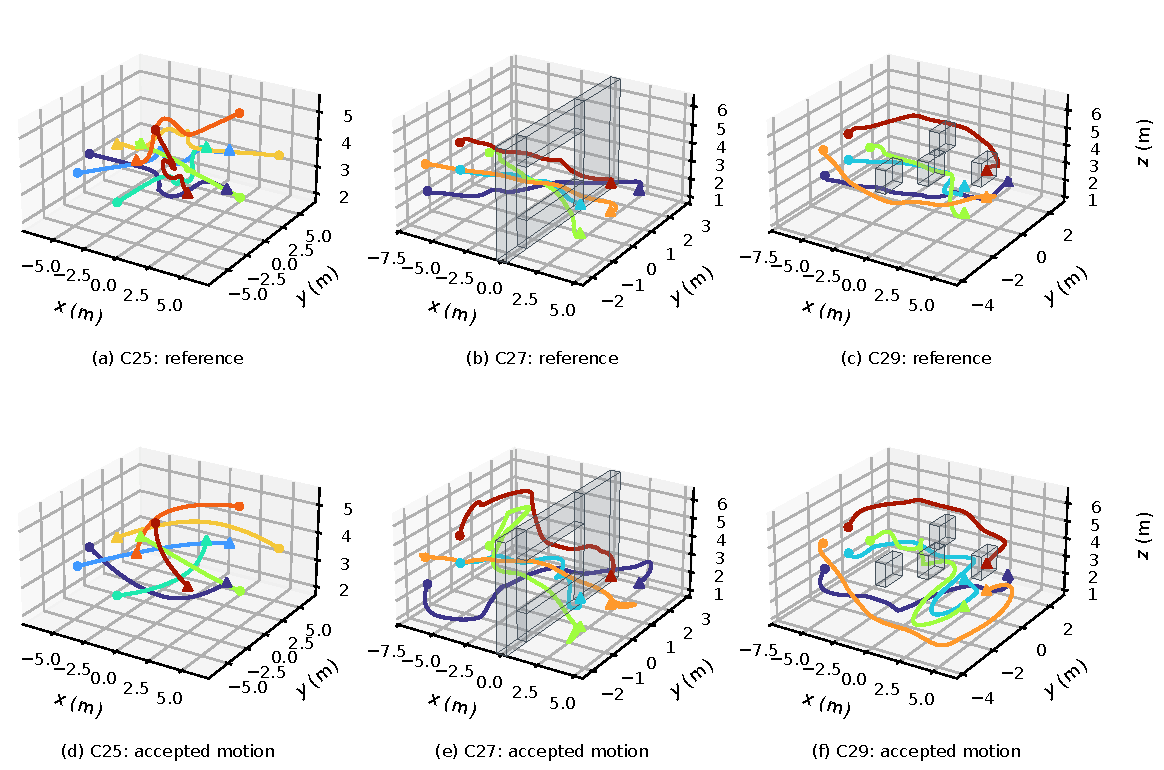
\includegraphics[width=\fulllength]{figures_revision/representative_motions.pdf}
\caption{Representative accepted cooperative motions with metric axes. Starts are circles, fixed goals are triangles, and colors identify UAVs. The full 30-scene overview is provided separately in the reproducibility package.\label{fig:scenes}}
\end{mdframed}
\end{adjustwidth}\end{figure}
\DIFaddend 


\DIFdelbegin 
\begin{figure}[p]
\begin{adjustwidth}{-\extralength}{0cm}
\begin{mdframed}[linecolor=RevisionRed,linewidth=.65pt,innerleftmargin=2pt,innerrightmargin=2pt,innertopmargin=3pt,innerbottommargin=3pt]
\color{RevisionRed}
\setlength{\textwidth}{\linewidth}\setlength{\fulllength}{\linewidth}

\centering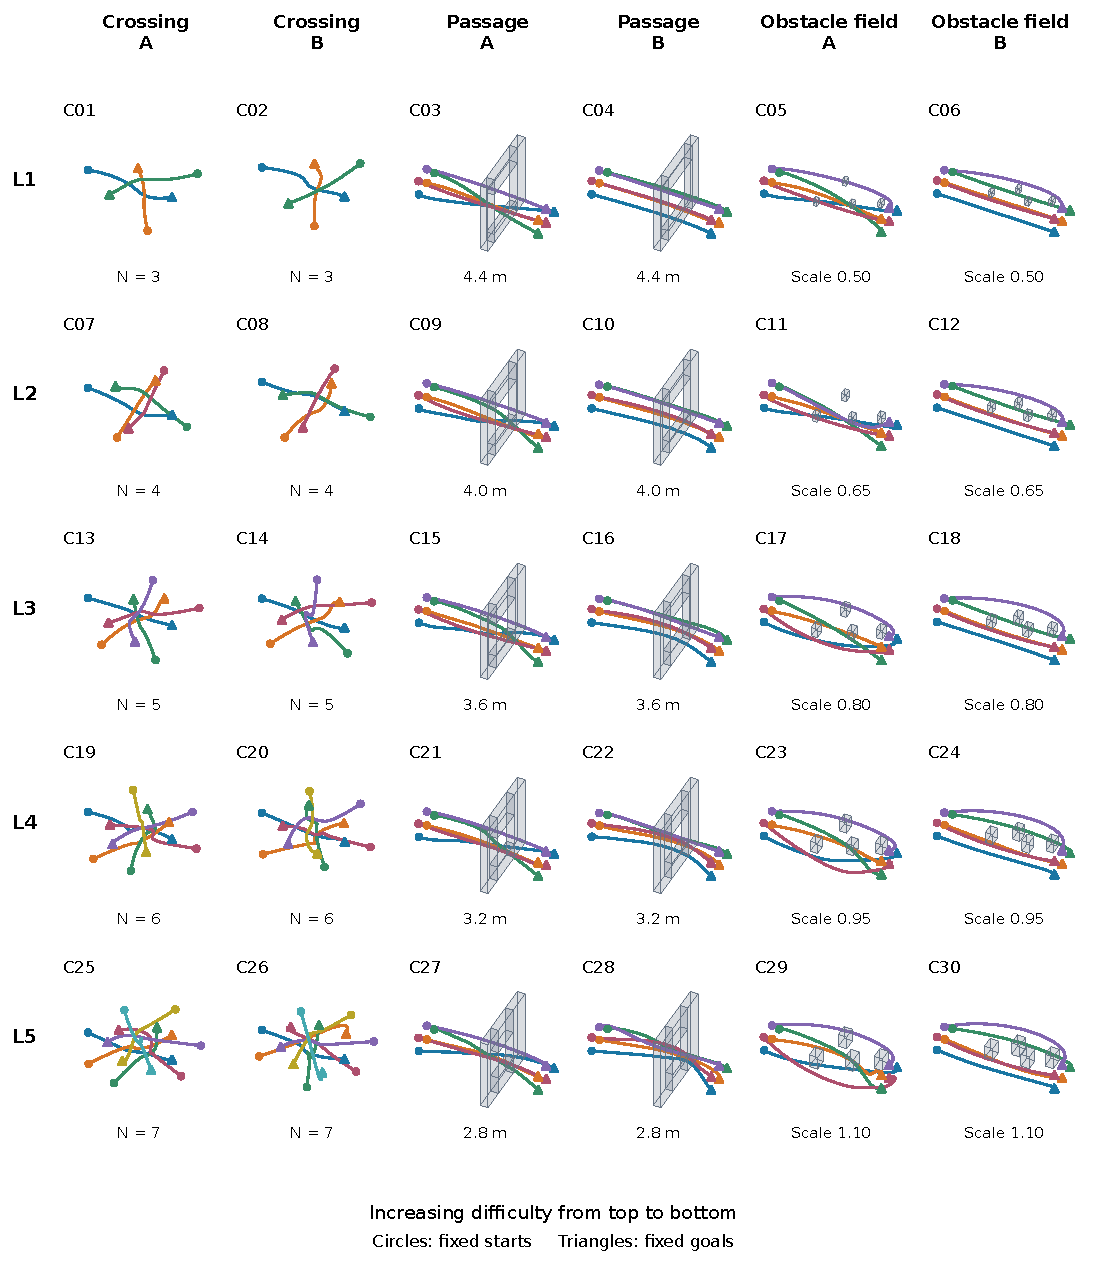
\includegraphics[width=\fulllength,height=20.6cm,keepaspectratio]{old_assets/figures_rest/all_cases.pdf}
\caption*{\textcolor{RevisionRed}{Deleted:} All 30 rest-to-rest cooperative motions. Rows indicate increasing difficulty; paired columns show the two realizations of each scene family. Small-panel axis ticks are omitted; metric enlarged views appear in Figure~\mbox{4}.}
\end{mdframed}
\end{adjustwidth}
\end{figure}

%DIFDELCMD < %%%
\DIFdelend \DIFaddbegin \begin{figure}[htbp]
\begin{adjustwidth}{-\extralength}{0cm}
\begin{mdframed}[linecolor=RevisionBlue,linewidth=.65pt,innerleftmargin=2pt,innerrightmargin=2pt,innertopmargin=3pt,innerbottommargin=3pt]
\color{RevisionBlue}
\setlength{\textwidth}{\linewidth}\setlength{\fulllength}{\linewidth}
\centering
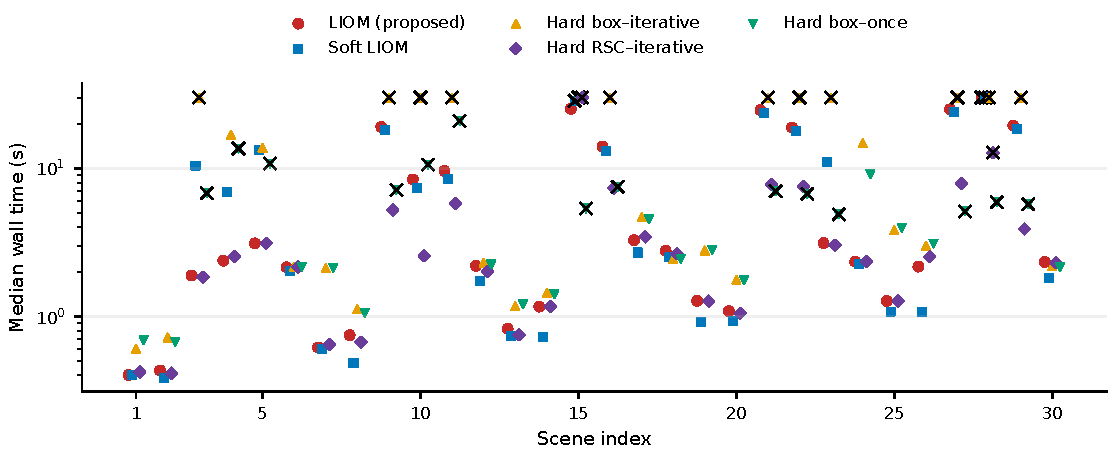
\includegraphics[width=\fulllength]{figures_revision/main_performance.pdf}
\caption{Main-benchmark computation. Per-scene median wall times use separated method positions and a logarithmic axis. Crosses mark a scene--method combination with an incomplete attempt among its three repetitions. All attempts enter the timing summaries.\label{fig:performance}}
\end{mdframed}
\end{adjustwidth}\end{figure}
\DIFaddend 



\DIFdelbegin 
\begin{figure}[p]
\begin{adjustwidth}{-\extralength}{0cm}
\begin{mdframed}[linecolor=RevisionRed,linewidth=.65pt,innerleftmargin=2pt,innerrightmargin=2pt,innertopmargin=3pt,innerbottommargin=3pt]
\color{RevisionRed}
\setlength{\textwidth}{\linewidth}\setlength{\fulllength}{\linewidth}

\centering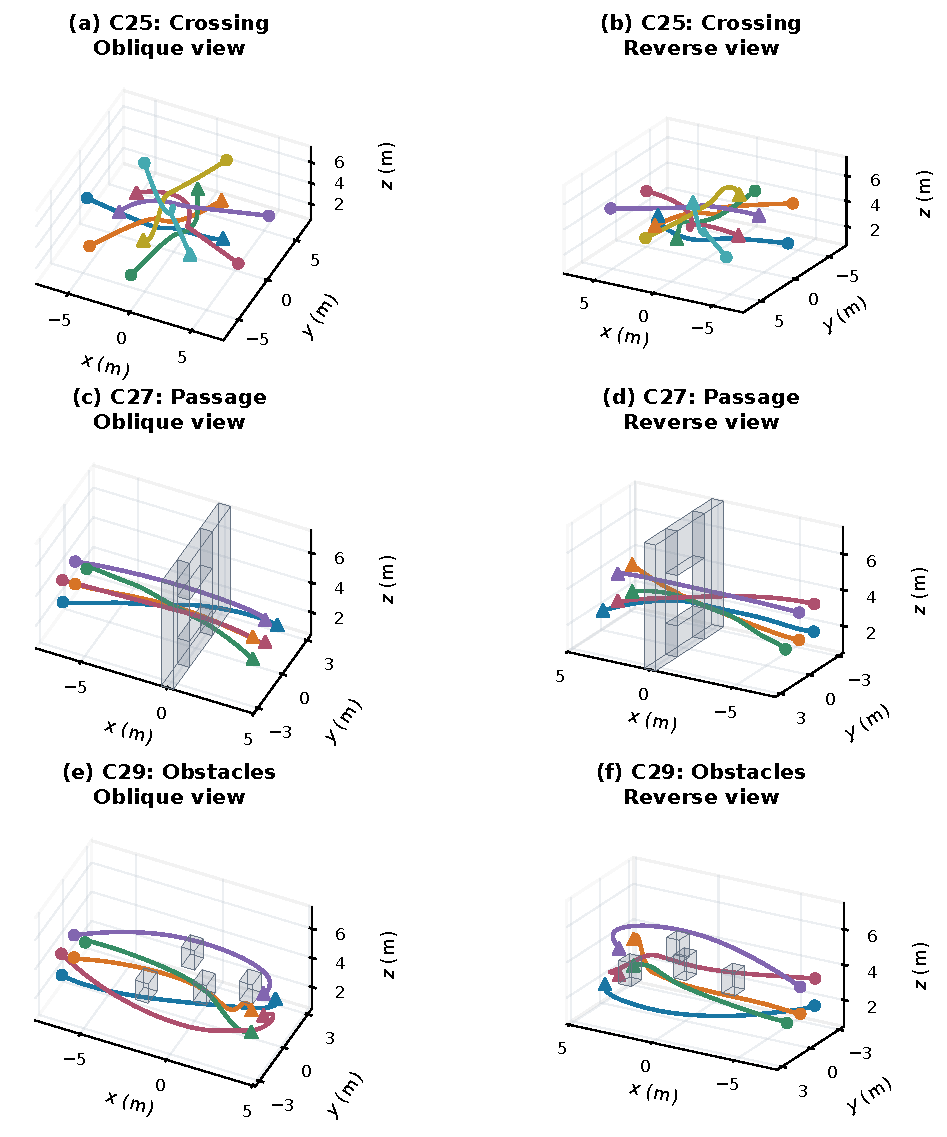
\includegraphics[width=\fulllength,height=20cm,keepaspectratio]{old_assets/figures_rest/scene_families.pdf}
\caption*{\textcolor{RevisionRed}{Deleted:} Three level-5 examples, each shown from an oblique and reverse view: C25, seven-UAV crossing; C27, five-UAV passage through a 2.8 m opening; and C29, the enlarged obstacle field. Obstacle surfaces are clipped to the displayed window; full geometry is used for planning and checking.}
\end{mdframed}
\end{adjustwidth}
\end{figure}

%DIFDELCMD < %%%
\DIFdelend \DIFaddbegin \begin{figure}[htbp]
\begin{adjustwidth}{-\extralength}{0cm}
\begin{mdframed}[linecolor=RevisionBlue,linewidth=.65pt,innerleftmargin=2pt,innerrightmargin=2pt,innertopmargin=3pt,innerbottommargin=3pt]
\color{RevisionBlue}
\setlength{\textwidth}{\linewidth}\setlength{\fulllength}{\linewidth}
\centering
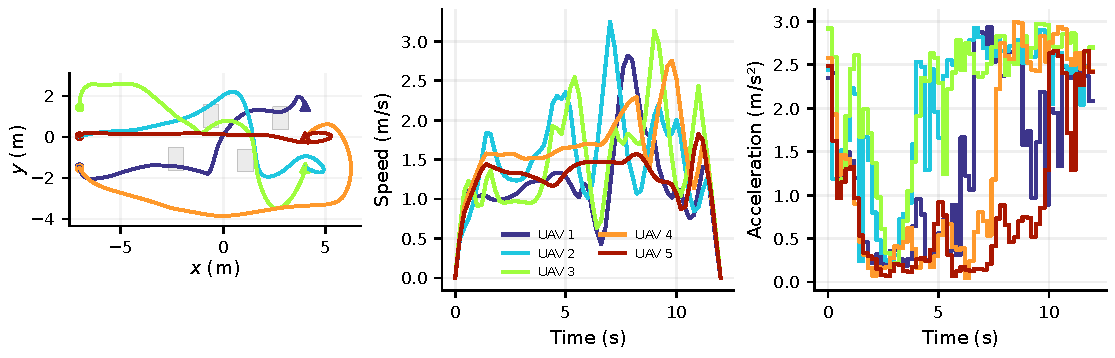
\includegraphics[width=\fulllength]{figures_revision/control_profiles.pdf}
\caption{Planar projection and individual UAV speed and acceleration histories for a representative accepted motion. Colors identify UAVs consistently across the panels.\label{fig:controls}}
\end{mdframed}
\end{adjustwidth}\end{figure}
\DIFaddend 




\DIFdelbegin \DIFdel{C27 illustrates how the spatial reference and final motion differ while maintaining the same task boundaries. Figure~\mbox{5} shows the reference and returned trajectories from an identical camera and gives two orthogonal projections. A projected overlap does not imply a simultaneous three-dimensional collision. Figure~\mbox{6} shows the corresponding continuous velocities and piecewise-constant acceleration controls for all five UAVs. }\DIFdelend \DIFaddbegin \subsection{\textcolor{RevisionBlue}{Recovery in Winding Counterflow Tasks}}
\DIFaddend 

\DIFdelbegin 
\begin{figure}[!htb]
\begin{adjustwidth}{-\extralength}{0cm}
\begin{mdframed}[linecolor=RevisionRed,linewidth=.65pt,innerleftmargin=2pt,innerrightmargin=2pt,innertopmargin=3pt,innerbottommargin=3pt]
\color{RevisionRed}
\setlength{\textwidth}{\linewidth}\setlength{\fulllength}{\linewidth}

\centering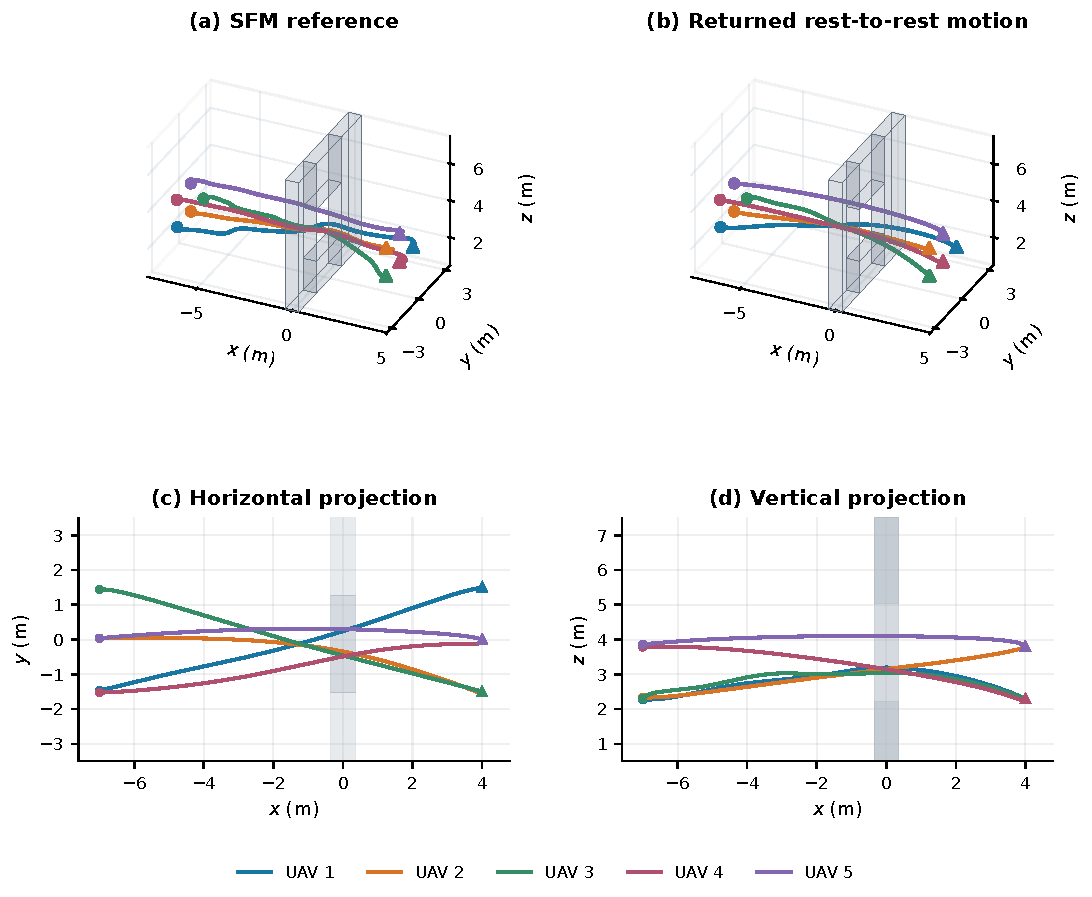
\includegraphics[width=\fulllength]{old_assets/figures_rest/passage_motion.pdf}
\caption*{\textcolor{RevisionRed}{Deleted:} C27 reference and returned motion, followed by horizontal and vertical projections. Both reference and output have a 12 s horizon and fixed start--goal assignments. Gray planar regions are obstacle projections.}
\end{mdframed}
\end{adjustwidth}
\end{figure}

%DIFDELCMD < 


\begin{figure}[htbp]
\begin{adjustwidth}{-\extralength}{0cm}
\begin{mdframed}[linecolor=RevisionRed,linewidth=.65pt,innerleftmargin=2pt,innerrightmargin=2pt,innertopmargin=3pt,innerbottommargin=3pt]
\color{RevisionRed}
\setlength{\textwidth}{\linewidth}\setlength{\fulllength}{\linewidth}

\centering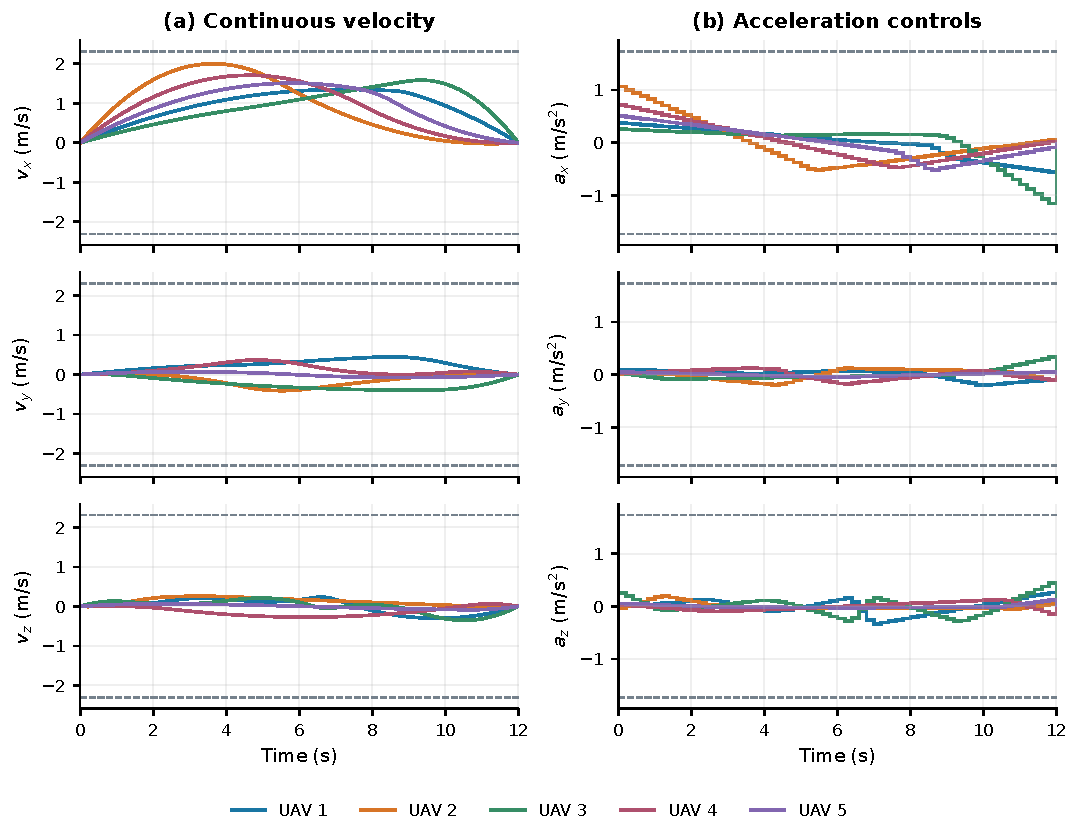
\includegraphics[width=\fulllength]{old_assets/figures_rest/passage_controls.pdf}
\caption*{\textcolor{RevisionRed}{Deleted:} C27 states and controls. Every velocity curve is continuous and begins and ends at zero. Acceleration is constant on each interval. Dashed lines mark the conservative Cartesian bounds.}
\end{mdframed}
\end{adjustwidth}
\end{figure}

%DIFDELCMD < 

%DIFDELCMD < \begin{samepage}
%DIFDELCMD < %%%
\DIFdel{The timing comparison in Figure~\mbox{7} uses the same admissible scalar rule for SFM and straight geometry. Profile amplitudes depend on their joint path lengths. The common horizon and endpoint-speed conditions provide a consistent timing basis for comparing the two geometric initializations. }%DIFDELCMD < \par\end{samepage}
%DIFDELCMD < 


\begin{figure}[htbp]
\begin{adjustwidth}{-\extralength}{0cm}
\begin{mdframed}[linecolor=RevisionRed,linewidth=.65pt,innerleftmargin=2pt,innerrightmargin=2pt,innertopmargin=3pt,innerbottommargin=3pt]
\color{RevisionRed}
\setlength{\textwidth}{\linewidth}\setlength{\fulllength}{\linewidth}

\centering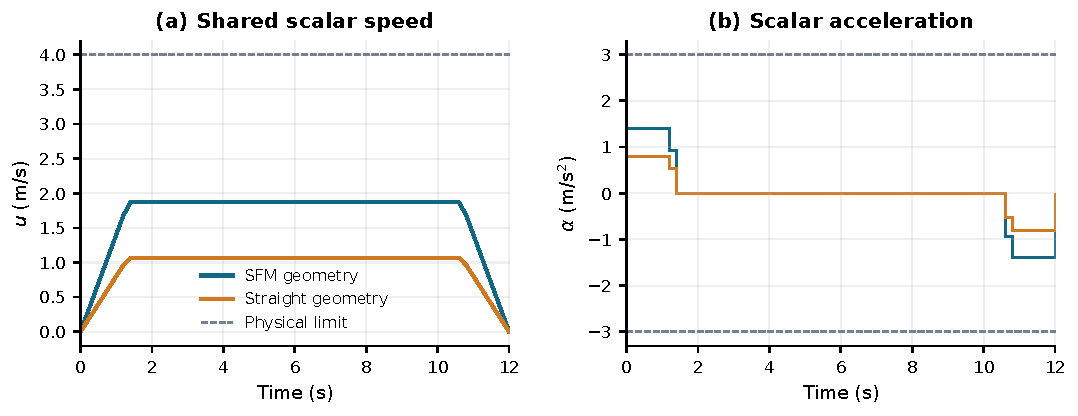
\includegraphics[width=\fulllength]{old_assets/figures_rest/reference_profiles.pdf}
\caption*{\textcolor{RevisionRed}{Deleted:} C27 scalar reference timing for the two geometric initializations. Both use the same scaled trapezoidal law, prescribed horizon, and zero boundary speeds; dashed lines show the common physical limits.}
\end{mdframed}
\end{adjustwidth}
\end{figure}

%DIFDELCMD < 


\par\noindent{\color{RevisionRed}\sout{\textbf{Initialization and Recovery Ablations}}}\par

%DIFDELCMD < 

%DIFDELCMD < %%%
\DIFdel{Proposed LIOM accepts }\DIFdelend \DIFaddbegin \label{sec:winding}
\DIFadd{Three full-height walls with alternating openings produce repeated turns and opposing traffic. The representative task contains five UAVs, 2.2 m openings, and a fixed 24 s flight horizon with $h=0.2$ s. The spatial and relative growth limits, motion envelope, footprint, acceptance thresholds, and }\DIFaddend 30 \DIFaddbegin \DIFadd{s planning budget remain unchanged. A common 0.325 m static-guide grid resolves the openings. Each method receives the same saved reference and is charged the same measured initialization time. Hard RSC--iterative retains its reconstruction loop.
}

\DIFadd{An exploratory search identified the task in Figure~\ref{fig:winding-recovery}. In the three initial paired executions of this task, proposed LIOM accepted the motion after five recovery rounds in 26.59--27.18 s. Soft LIOM also accepted all three executions, taking 25.33--25.72 s. Hard RSC--iterative completed eight reconstruction rounds per execution without acceptance within the budget. These repetitions characterize one physical task. Section~\ref{sec:external} reports a further paired execution alongside the nonlinear and sequential-convex methods. The accepted motion has minimum center separation 1.086 m, minimum obstacle surface clearance 0.495 m, maximum speed 3.577 m}\DIFaddend /\DIFdelbegin \DIFdel{30 scenes, Straight + LIOM accepts 7}\DIFdelend \DIFaddbegin \DIFadd{s, and maximum acceleration 2.990 m}\DIFaddend /\DIFdelbegin \DIFdel{30, and Hard-once accepts 29}\DIFdelend \DIFaddbegin \DIFadd{s$^2$; the respective requirements are 0.60 m, 0.10 m, 4 m}\DIFaddend /\DIFdelbegin \DIFdel{30. Figure~\mbox{8} relates these outcomes to per-case CPU time and wall-clock deadlines. Guided reference construction and subsequent guide availability supply useful static detours and passing patterns, increasing success and reducing computation relative to the straight-reference variant. The one-shot formulation is efficient on compatible initial corridors; Proposed LIOM additionally accepts C26 after a second solve. }\DIFdelend \DIFaddbegin \DIFadd{s, and 3 m/s$^2$.
}\DIFaddend 

\DIFdelbegin 
\begin{figure}[htbp]
\begin{adjustwidth}{-\extralength}{0cm}
\begin{mdframed}[linecolor=RevisionRed,linewidth=.65pt,innerleftmargin=2pt,innerrightmargin=2pt,innertopmargin=3pt,innerbottommargin=3pt]
\color{RevisionRed}
\setlength{\textwidth}{\linewidth}\setlength{\fulllength}{\linewidth}

\centering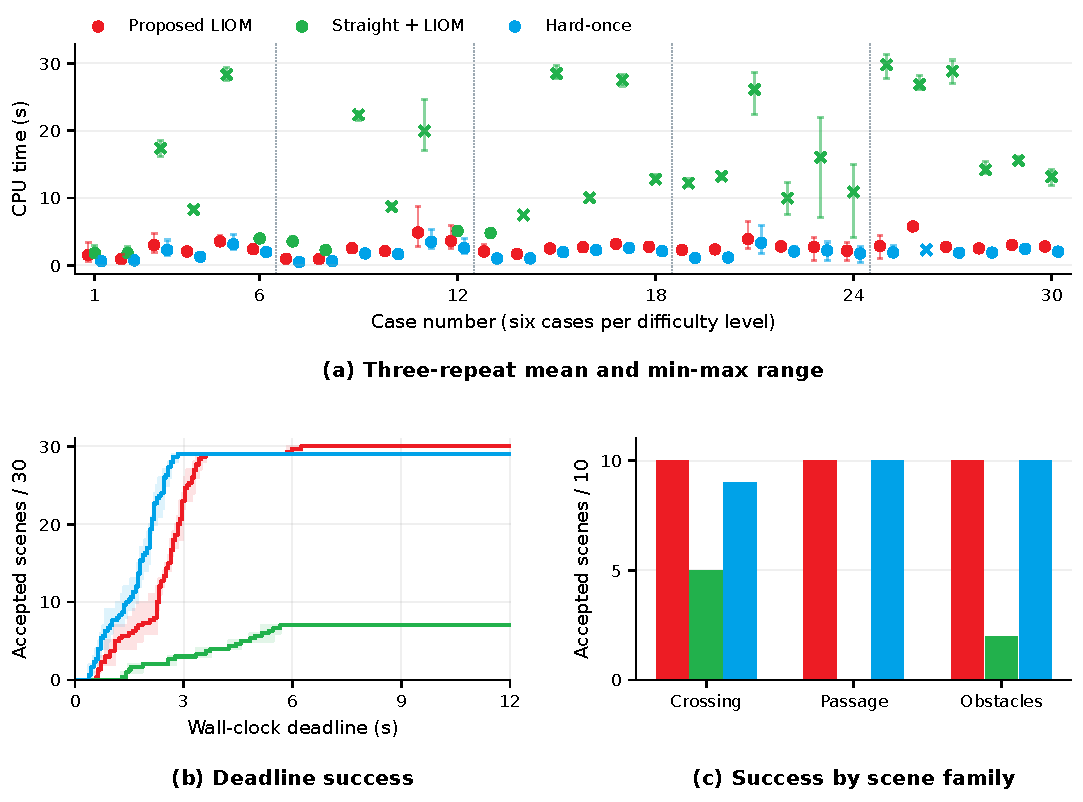
\includegraphics[width=\fulllength]{old_assets/figures_rest/performance.pdf}
\caption*{\textcolor{RevisionRed}{Deleted:} Initialization and recovery ablation batch. (a) Per-case CPU means and min--max ranges over three repetitions; circles mark acceptance and crosses failure. (b) Accepted scenes by wall-clock deadline, with repetition ranges shaded. (c) Scene-family acceptance. Failed attempts remain in timing statistics.}
\end{mdframed}
\end{adjustwidth}
\end{figure}

%DIFDELCMD < %%%
\DIFdelend \DIFaddbegin \DIFadd{An independent phase-I linear program minimizes a common row-scaled violation of the initial hard-RSC constraints. Its primal and dual objectives both equal 0.21915, with primal residual below $5\times10^{-14}$ and dual stationarity residual below $2\times10^{-17}$. Removing the relative rows alone, or the kinematic equalities alone, gives zero phase-I objective. These diagnostic checks identify an incompatibility between the selected relative restrictions and exact motion consistency. The complete returned motion satisfies both requirements after reconstruction. The diagnostic relaxations are used only to identify the conflict.
}\DIFaddend 


\DIFdelbegin \DIFdel{The flight duration is fixed at 12 sfor every variant. The computation shown in Figure~\mbox{8} precedes execution of that motion. }\DIFdelend \DIFaddbegin \begin{figure}[htbp]
\begin{adjustwidth}{-\extralength}{0cm}
\begin{mdframed}[linecolor=RevisionBlue,linewidth=.65pt,innerleftmargin=2pt,innerrightmargin=2pt,innertopmargin=3pt,innerbottommargin=3pt]
\color{RevisionBlue}
\setlength{\textwidth}{\linewidth}\setlength{\fulllength}{\linewidth}
\centering
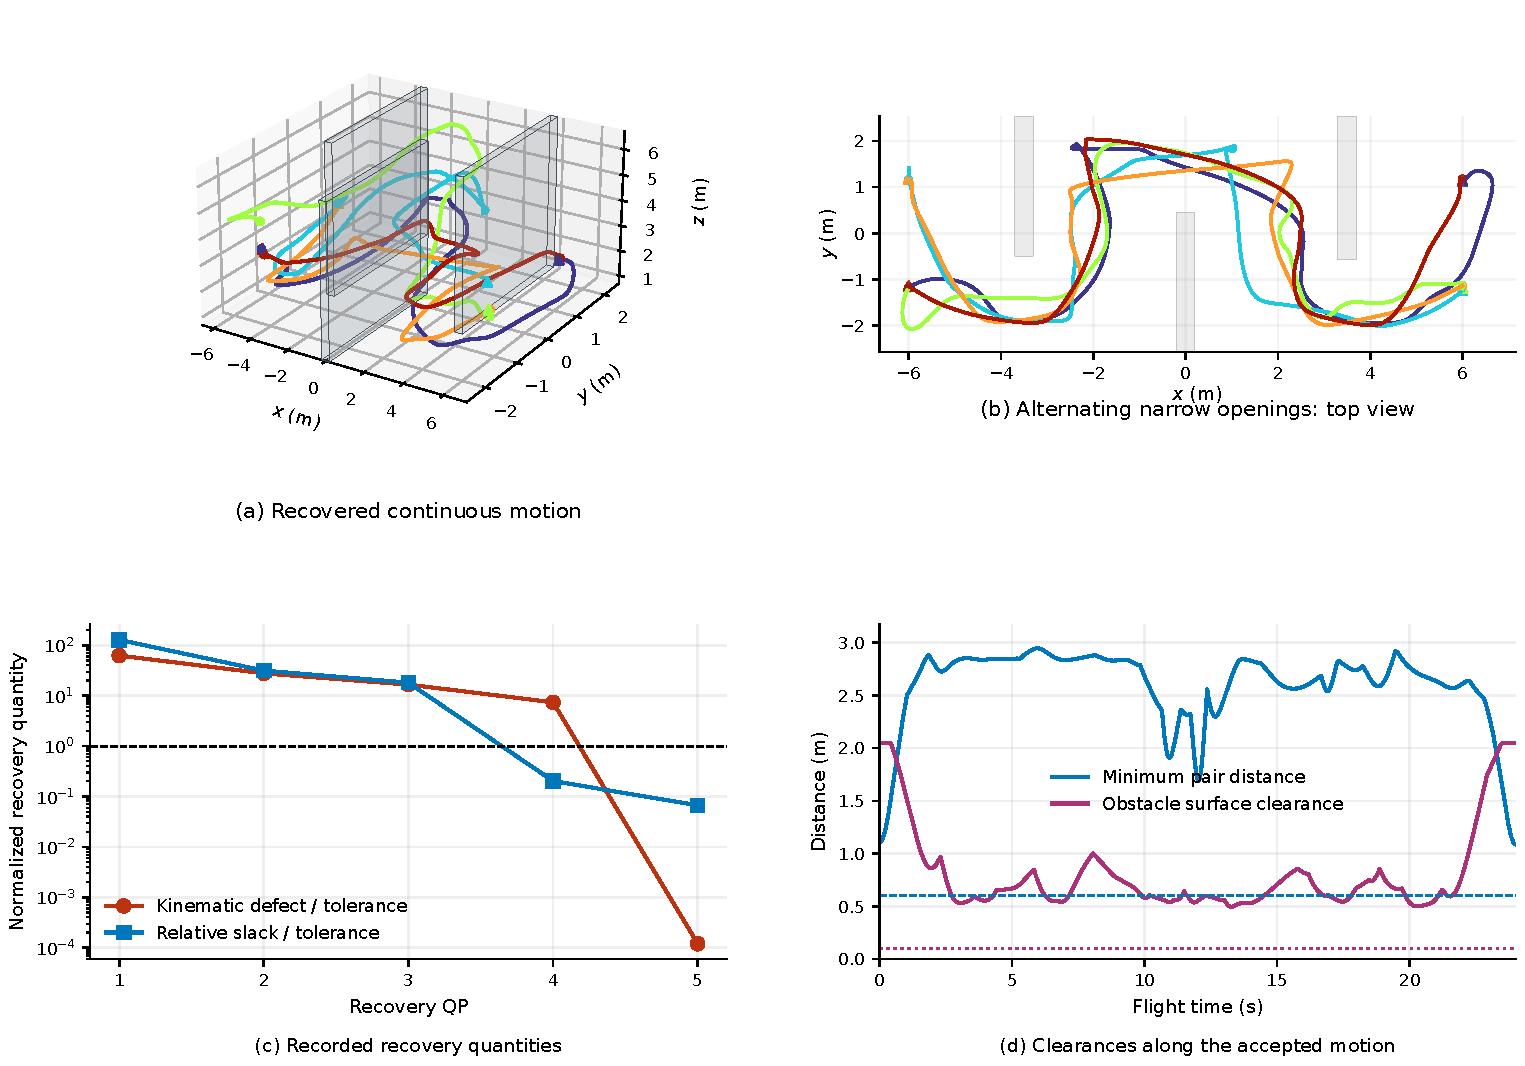
\includegraphics[width=\fulllength]{figures_revision/winding_recovery_case.pdf}
\caption{Recovery in a winding counterflow task. Colors identify UAVs. The recovery quantities are divided by their acceptance thresholds; the dashed unit line marks numerical recovery. The clearance curves visualize the integrated motion, whose acceptance is determined by complete-interval checks.\label{fig:winding-recovery}}
\end{mdframed}
\end{adjustwidth}\end{figure}
\DIFaddend 


\DIFdelbegin 
\par\noindent{\color{RevisionRed}\sout{\textbf{Recovery from Incompatible Initial Corridors}}}\par

%DIFDELCMD < %%%
\DIFdelend \DIFaddbegin \DIFadd{A separate set of 12 previously untested random layouts contains a second recovered task whose initial hard QP has matching phase-I primal and dual objectives of 0.35420. The proposed method returns a checked motion for this task, while iterative hard RSC exhausts the common budget. This independently generated case supports the same conflict mechanism. The complete 12-layout outcomes and all exploratory records accompany the data.
}\DIFaddend 

\DIFdelbegin \DIFdel{Proposed LIOM accepts 29 main-benchmark cases after one solve and C26 after two. In C26, the first solve gives $D=1.36\times10^{-2}$ m$^2$ and $S=2.85\times10^{-2}$ m. Both exceed their recovery thresholds. After the weights increase to 2, 000 and the corridors are rebuilt, the second candidate reaches $D=4.85\times10^{-9}$ m$^2$ and $S=7.91\times10^{-11}$ m; its reconstructed motion passes the complete-interval checks.
}%DIFDELCMD < 

%DIFDELCMD < \begin{samepage}
%DIFDELCMD < %%%
\DIFdel{C26's initial hard-box infeasibility was independently confirmed with HiGHS~\mbox{[orig. 37]}.
For the row-scaled linear system $Ax\leq b$, a Phase-I program gives a minimum common relaxation of $1.5175\times10^{-2}$. Nonnegative dual multipliers satisfy $\|A^\top y\|_\infty=2.08\times10^{-17}$ and $b^\top y=-1.5175\times10^{-2}$, with a positive contradiction margin after accounting for finite state bounds. This numerical certificate concerns the selected initial boxes. The accepted second-round trajectory demonstrates recovery of the unchanged physical task through revised local geometry.
}%DIFDELCMD < \par\end{samepage}
%DIFDELCMD < 

%DIFDELCMD < %%%
\DIFdel{Together, the ablations show the roles of a coordinated reference and the complete recovery procedure. The pressure tests below examine the latter across multiple layouts and degrees of local restriction}\DIFdelend \DIFaddbegin \DIFadd{Figure~\ref{fig:winding-map} varies physical opening width, team size, and prescribed flight time around the identified geometry. The nominal corridor-growth limits are unchanged. Both methods accept the three-UAV tasks. With five UAVs and 2.2 m openings, proposed LIOM additionally accepts the 24 s and 28 s tasks. Widening the openings permits both methods to succeed. The map locates the additional recovery region under physical congestion; it also shows where neither method returns an accepted motion within the common budget}\DIFaddend .

\DIFdelbegin 
\par\noindent{\color{RevisionRed}\sout{\textbf{Task-Matched Computational Comparison}}}\par

%DIFDELCMD < %%%
\DIFdelend \DIFaddbegin \begin{figure}[htbp]
\begin{adjustwidth}{-\extralength}{0cm}
\begin{mdframed}[linecolor=RevisionBlue,linewidth=.65pt,innerleftmargin=2pt,innerrightmargin=2pt,innertopmargin=3pt,innerbottommargin=3pt]
\color{RevisionBlue}
\setlength{\textwidth}{\linewidth}\setlength{\fulllength}{\linewidth}
\centering
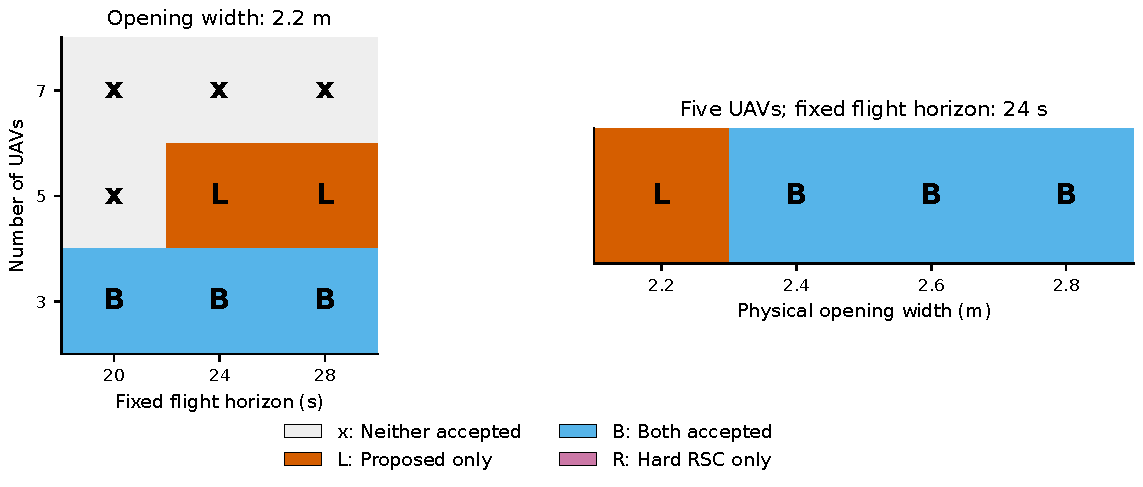
\includegraphics[width=\fulllength]{figures_revision/physical_recovery_map.pdf}
\caption{Exploratory physical-parameter map around the same winding layout. Letters supplement color: B, both accepted; L, proposed LIOM only; R, Hard RSC--iterative only; x, neither accepted. Twelve distinct settings are evaluated; the five-UAV, 24 s, 2.2 m setting appears in both panels. Every setting uses the same reference for both methods and the same 30 s budget.\label{fig:winding-map}}
\end{mdframed}
\end{adjustwidth}\end{figure}
\DIFaddend 






\DIFaddbegin \subsection{\textcolor{RevisionBlue}{Task-Matched Nonlinear and Sequential Convex Comparisons}}

\DIFaddend \label{sec:external}
\DIFdelbegin \DIFdel{Four computational baselines use the common guided reference, hard integration equations, and the same physical taskand acceptance tests:
}%DIFDELCMD < \begin{samepage}
%DIFDELCMD < \begin{itemize}
%DIFDELCMD < \item %%%
\DIFdel{\textbf{ASCO-3D}: adaptive risk-range selection of nonlinear collision constraints~\mbox{\cite{li2021asco}} , with rangecontraction after failed reduced solves and expansion after full-check violations. }%DIFDELCMD < \item %%%
\DIFdel{\textbf{Hard RSC-QP}: spatial boxes and hard relative separating half-spaces based on the relative safe flight corridor principle~\mbox{\cite{park2021}}. This fixed-horizon, centralized variant isolates the hard-corridor component; the cited online planner additionally uses slack and reciprocal avoidance.
}%DIFDELCMD < \item %%%
\DIFdel{\textbf{SCP-3D}: successive affine lower bounds on squared separation distances~\mbox{\cite{augugliaro2012}} }\DIFdelend \DIFaddbegin \DIFadd{Three additional strategies are adapted to the same UAV task}\DIFaddend . \DIFdelbegin %DIFDELCMD < \item %%%
\DIFdel{\textbf{Direct NLP}: simultaneous enforcement of all nonlinear distance constraints in one solve.}%DIFDELCMD < \end{itemize}
%DIFDELCMD < \par\end{samepage}
%DIFDELCMD < %%%
\DIFdel{For a reference relative position $\mathbf r^0$ and padded separation $R$, the two affine representations are
}%DIFDELCMD < 



\begin{mdframed}[nobreak=true,linecolor=RevisionRed,linewidth=.65pt,innerleftmargin=5pt,innerrightmargin=5pt,innertopmargin=2pt,innerbottommargin=2pt,skipabove=6pt,skipbelow=6pt]
\color{RevisionRed}
{\scriptsize Deleted mathematical display}\par
\begin{equation*}
 \underbrace{\frac{(\mathbf r^0)^\top\mathbf r}{\norm{\mathbf r^0}_2}\geq R}_{\text{Hard RSC-QP}},\qquad
 \underbrace{2(\mathbf r^0)^\top\mathbf r\geq R^2+\norm{\mathbf r^0}_2^2}_{\text{SCP-3D}}.
\end{equation*}
\end{mdframed}


%DIFDELCMD < 

%DIFDELCMD < %%%
\DIFdel{Hard RSC-QP uses padded nodes and the common spatial boxes. The other baselines use }\DIFdelend \DIFaddbegin \DIFadd{ASCO-3D~\mbox{\cite{li2021asco}} changes the active collision-risk range, retaining the preceding successful reference after a failed reduced solve. Direct NLP imposes all sampled collision restrictions simultaneously. SCP-3D~\mbox{\cite{augugliaro2012}} uses the distance-norm tangent restrictions of Eq.~(17) in~\mbox{\cite{augugliaro2012}}, with supporting planes for the static boxes. All use hard integration equations, the same polyhedral motion limits, fixed endpoints, fixed horizon, and control-effort objective. Collision restrictions are evaluated at }\DIFaddend quarter-interval \DIFdelbegin \DIFdel{samples, reachable-displacement padding over $h/8$, and spherical-UAV/AABB distances or their linearizations. Signed distance preserves a penetration gradient for nonlinear intermediate candidates. Each accepted output }\DIFdelend \DIFaddbegin \DIFadd{arc samples with reachable-motion padding. The returned motion }\DIFaddend undergoes the same \DIFaddbegin \DIFadd{endpoint reconstruction and }\DIFaddend complete-interval \DIFdelbegin \DIFdel{check.
These choices compare local constraint representations under identical endpoints, motion limits, and flight duration.
}\DIFdelend \DIFaddbegin \DIFadd{acceptance tests as LIOM.
}\DIFaddend 

\DIFdelbegin \DIFdel{All baselines use the nominal 30 s budget and up to 6,000 inner iterations per solve. ASCO-3D limits each reduced solve to 5 CPU seconds; the others receive the remaining budget. Iterative strategies allow at most 30 solves. }\DIFdelend \DIFaddbegin \DIFadd{The nonlinear ASCO and direct-NLP instances use CasADi~\mbox{\cite{andersson2019}} and Ipopt~\mbox{\cite{wachter2006}} with the ma57 linear solver. Every quadratic subproblem uses OSQP. SCP assembles its sparse matrices directly; ASCO iterations without active nonlinear rows also use the QP backend. }\DIFaddend ASCO's \DIFaddbegin \DIFadd{original }\DIFaddend risk-range \DIFdelbegin \DIFdel{parameters }\DIFdelend \DIFaddbegin \DIFadd{lengths }\DIFaddend are scaled by the ratio of UAV radius to the \DIFdelbegin \DIFdel{original covering-disc radius }\DIFdelend \DIFaddbegin \DIFadd{vehicle-disc radius in the source implementation. Its update rule and 50-round ceiling are retained; the common 30 s budget governs the comparison.
}

\DIFadd{The paired study comprises six original benchmark tasks, both winding layouts, and 15- }\DIFaddend and \DIFdelbegin \DIFdel{remain fixed across scenes.
Three paired batches rerun Proposed LIOM and Hard-once alongside the four baselines .
}\DIFdelend \DIFaddbegin \DIFadd{20-UAV tasks. The winding tasks use $T_f=24$ s and $K=120$; the remaining tasks use $T_f=12$ s and $K=60$. The methods are evaluated serially. Each method receives the identical saved reference and is charged its measured generation time. The comparison records one execution per task--method pair. The nonlinear baselines are rerun with ma57; the unchanged QP implementations retain their recorded measurements. Construction, solution, and final checking all enter the reported time, including calls that overrun the nominal stopping budget.
}\DIFaddend 



\DIFdelbegin 
\begin{table}[htbp]
\begin{adjustwidth}{-\extralength}{0cm}
\begin{mdframed}[linecolor=RevisionRed,linewidth=.65pt,innerleftmargin=2pt,innerrightmargin=2pt,innertopmargin=3pt,innerbottommargin=3pt]
\color{RevisionRed}
\setlength{\textwidth}{\linewidth}\setlength{\fulllength}{\linewidth}

\caption*{\textcolor{RevisionRed}{Deleted:} Paired computational comparison on the 30 main-benchmark scenes. Proposed LIOM is the complete method developed in this paper.}

\small\setlength{\tabcolsep}{4pt}
\begin{tabularx}{\fulllength}{Yrrrrr}
\toprule Method & Accepted & Within 30 s & CPU mean (s) & Wall mean (s) & Wall P95 (s) \\
\midrule
\textbf{Proposed LIOM} & 30/30 & 30/30 & $1.44\pm0.43$ & $1.31\pm0.40$ & 3.03 \\
Hard-once & 29/30 & 29/30 & $0.92\pm0.31$ & $0.82\pm0.30$ & 2.45 \\
ASCO-3D & 30/30 & 30/30 & $2.14\pm0.53$ & $2.12\pm0.59$ & 6.74 \\
Hard RSC-QP & 30/30 & 30/30 & $1.01\pm0.26$ & $0.91\pm0.25$ & 2.48 \\
SCP-3D & 30/30 & 30/30 & $2.09\pm0.45$ & $2.02\pm0.48$ & 4.87 \\
Direct NLP & 30/30 & 23--29/30 & $11.38\pm2.34$ & $12.01\pm2.75$ & 31.70 \\
\bottomrule\end{tabularx}
\par\vspace{3pt}\footnotesize Counts refer to 30 distinct scenes. The deadline column gives the range across three repetitions; accepted counts are identical in all repetitions. Timing includes every attempt. $\pm$ denotes the SD of the three batch means; P95 uses all 90 attempts per method.


\end{mdframed}
\end{adjustwidth}
\end{table}

%DIFDELCMD < %%%
\DIFdelend \DIFaddbegin \begin{table}[htbp]
\begin{adjustwidth}{-\extralength}{0cm}
\begin{mdframed}[linecolor=RevisionBlue,linewidth=.65pt,innerleftmargin=2pt,innerrightmargin=2pt,innertopmargin=3pt,innerbottommargin=3pt]
\color{RevisionBlue}
\setlength{\textwidth}{\linewidth}\setlength{\fulllength}{\linewidth}

\caption{Task-matched planning times in seconds, including recorded initialization. LIOM uses the original 1 s hard entry in this comparison; the nonlinear columns are rerun with Ipopt/ma57. A cross denotes no accepted motion; $\dagger$ denotes an accepted motion returned after the nominal 30 s budget. Each entry is one recorded execution.\label{tab:external}}
\small\begin{tabularx}{\fulllength}{Ycrrrrr}\toprule
Task & $N$ & \textbf{LIOM (1 s)} & Hard RSC & ASCO-3D & Direct NLP & SCP-3D\\\midrule
C01 & 3 & \textbf{1.72} & 0.90 & 5.25 & 2.61 & 1.77\\
C03 & 5 & \textbf{1.51} & 1.42 & 3.50 & 29.05 & 3.27\\
C05 & 5 & \textbf{3.14} & 3.38 & 16.33 & 33.58$^{\dagger}$ & 5.47\\
C25 & 7 & \textbf{1.29} & 1.23 & 21.35 & 9.33 & 12.52\\
C27 & 5 & \textbf{24.35} & 7.55 & 8.61 & 27.79 & 5.41\\
C29 & 5 & \textbf{19.54} & 4.07 & 15.06 & 27.16 & 10.32\\
Winding A & 5 & \textbf{26.36} & 25.14 & $\times$\,33.72 & $\times$\,47.10 & $\times$\,28.41\\
Winding B & 5 & \textbf{31.92$^{\dagger}$} & $\times$\,30.07 & $\times$\,31.50 & $\times$\,31.36 & $\times$\,30.05\\
15-UAV & 15 & \textbf{27.49} & 29.97 & $\times$\,34.07 & 59.34$^{\dagger}$ & 19.91\\
20-UAV & 20 & \textbf{30.12$^{\dagger}$} & 27.70 & $\times$\,31.27 & $\times$\,106.75 & $\times$\,30.06\\
\bottomrule\end{tabularx}
\end{mdframed}
\end{adjustwidth}\end{table}
\DIFaddend 





Table~\DIFdelbegin \DIFdel{\mbox{6} shows that Proposed LIOM accepts all scenes at a mean CPU time of 1.44 s, below ASCO-3D, SCP-3D, and Direct NLP. The accepted outputs also meet the 30 s deadline in every repetition. ASCO'sconstraint selection reduces the cost of the all-distance nonlinear formulation, while the corridor and affine-separation methods exploit the quadratic structure of fixed-horizon translational planning. }\DIFdelend \DIFaddbegin \DIFadd{\ref{tab:external} reports the ma57 comparison. LIOM completes C01, C03, C05, and C25 in 1.29--3.14 s. In C27, LIOM returns an accepted motion in 24.35 s, while ASCO, hard RSC, and SCP complete the same task in 8.61, 7.55, and 5.41 s. The ma57 direct-NLP solve also accepts C27, in 27.79 s. These results show how the direct hard path and the recovery path distribute computation across tasks.
}\DIFaddend 

\DIFdelbegin \DIFdel{Hard RSC-QP accepts all 30 scenes at a mean wall time of 0.91 s, compared with 1.31 sfor Proposed LIOM }\DIFdelend \DIFaddbegin \DIFadd{Winding A combines three alternating openings with opposing traffic. LIOM and iterative hard RSC return accepted motions in 26.36 and 25.14 s in this comparison. ASCO's candidate motions continue to fail collision checks when its budget is exhausted; SCP reports infeasibility for its initial tangent problem. The hard-RSC result supplements the earlier repetitions in Section~\ref{sec:winding}. The positive phase-I certificate identifies an incompatible initial local problem, and later reconstruction can reach a feasible corridor configuration. In Winding B, LIOM produces a physically accepted motion at 31.92 s; the ma57 baselines and the other hard comparisons return no accepted motion in their recorded attempts. The late LIOM output is marked explicitly in the table}\DIFaddend .
\DIFdelbegin \DIFdel{It also accepts C26 using its initial half-spaces, illustrating how a different local region can resolve a particular incompatibility before iteration begins. The pressure tests examine the complementary requirement: continuing refinement when the local region conflicts with the fixed-horizon task.
}\DIFdelend 

\DIFdelbegin \DIFdel{The deadline column separates accepted motion from timely completion}\DIFdelend \DIFaddbegin \DIFadd{For the 15-UAV task, LIOM, hard RSC, and SCP complete in 27.49, 29.97, and 19.91 s}\DIFaddend . Direct NLP returns \DIFdelbegin \DIFdel{accepted outputs for all scenes, with 29, 29, and 23 completed within 30 sacross the three repetitions; its wall-time P95 is 31.70 s. The remaining methods' accepted main-benchmark outputs finish within 30 s}\DIFdelend \DIFaddbegin \DIFadd{an accepted motion after its nominal budget, and ASCO ends without an accepted motion. At 20 UAVs, hard RSC completes in 27.70 s and LIOM returns an accepted motion at 30.12 s. Symbolic construction consumes the remaining budget in the two winding direct-NLP tasks and the 20-UAV direct-NLP task. The source records separate construction, numerical solution, and physical checking}\DIFaddend .






\DIFdelbegin 
\par\noindent{\color{RevisionRed}\sout{\textbf{Recovery under Time and Corridor Pressure}}}\par

%DIFDELCMD < %%%
\DIFdelend \DIFaddbegin \subsection{\textcolor{RevisionBlue}{Physical Congestion and Computational Scaling}}
\DIFaddend 

\DIFdelbegin %DIFDELCMD < \label{sec:stress}
%DIFDELCMD < %%%
\DIFdel{The pressure tests use the five-, six-, and seven-UAV crossing layouts C13/C14, C19/C20, and C25/C26. One sweep }\DIFdelend \DIFaddbegin \label{sec:scaling}

\DIFadd{The physical-congestion study varies crossing-team size, opening width, and obstacle dimensions while retaining the nominal corridor-growth limits. Figure~\ref{fig:physical} reports the mean computation in each group, including attempts that reach the stopping budget. The 30 s plateau marks termination at the nominal computational budget. These measurements characterize computational load, while the paired winding tasks provide direct evidence of recovery from incompatible local constraints.
}



\begin{figure}[htbp]
\begin{adjustwidth}{-\extralength}{0cm}
\begin{mdframed}[linecolor=RevisionBlue,linewidth=.65pt,innerleftmargin=2pt,innerrightmargin=2pt,innertopmargin=3pt,innerbottommargin=3pt]
\color{RevisionBlue}
\setlength{\textwidth}{\linewidth}\setlength{\fulllength}{\linewidth}
\centering
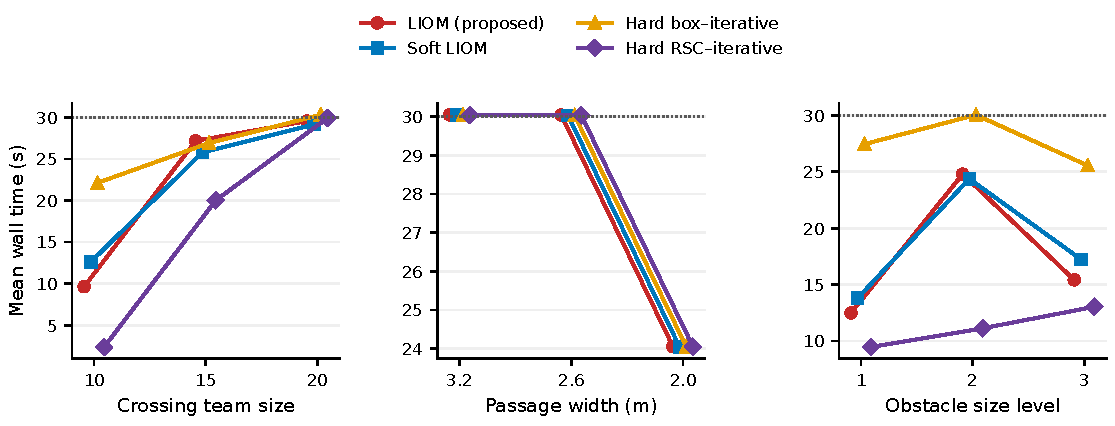
\includegraphics[width=\fulllength]{figures_revision/physical_congestion.pdf}
\caption{Computation under physical congestion with fixed corridor-growth settings. Panels vary crossing-team size, passage width, and obstacle size. Symbols distinguish methods in grayscale, and all attempts enter each mean.\label{fig:physical}}
\end{mdframed}
\end{adjustwidth}\end{figure}


\DIFadd{The grid study combines $N\in\{5,10,15,20\}$ and $K\in\{30,60,90\}$ with two predetermined realizations per combination. This separates team growth from discretization changes. Figure~\ref{fig:scaling} relates measured computation to problem size and shows the stage breakdown. The number of pair restrictions can decrease substantially after spatial-box screening, while complete-interval validation still checks all pairs.
}


\begin{table}[htbp]
\begin{adjustwidth}{-\extralength}{0cm}
\begin{mdframed}[linecolor=RevisionBlue,linewidth=.65pt,innerleftmargin=2pt,innerrightmargin=2pt,innertopmargin=3pt,innerbottommargin=3pt]
\color{RevisionBlue}
\setlength{\textwidth}{\linewidth}\setlength{\fulllength}{\linewidth}

\caption{Team/grid scaling over two realizations per setting. Mean wall times include all attempts. Variables and rows are the proposed method's mean maximum dimensions; coupling varies with the spatial boxes.\label{tab:scaling-new}}
\centering\small
\begin{tabular}{lrrrrr}\toprule
$N$ & $K$ & LIOM wall (s) & Hard RSC wall (s) & Variables & Rows\\\midrule
5 & 30 & 0.16 & 0.13 & 870 & 7,710\\
5 & 60 & 0.21 & 0.18 & 1,770 & 15,497\\
5 & 90 & 0.46 & 0.44 & 2,670 & 23,285\\
10 & 30 & 21.82 & 9.92 & 2,653 & 19,641\\
10 & 60 & 1.01 & 1.01 & 3,540 & 32,012\\
10 & 90 & 11.13 & 3.66 & 7,759 & 57,477\\
15 & 30 & 30.05 & 25.00 & 4,770 & 34,200\\
15 & 60 & 22.38 & 5.95 & 9,249 & 66,477\\
15 & 90 & 25.88 & 27.80 & 13,698 & 98,568\\
20 & 30 & 30.04 & 30.02 & 7,476 & 52,299\\
20 & 60 & 26.98 & 21.87 & 14,379 & 100,914\\
20 & 90 & 21.75 & 30.06 & 21,233 & 149,238\\
\bottomrule\end{tabular}
\end{mdframed}
\end{adjustwidth}
\end{table}




\begin{figure}[htbp]
\begin{adjustwidth}{-\extralength}{0cm}
\begin{mdframed}[linecolor=RevisionBlue,linewidth=.65pt,innerleftmargin=2pt,innerrightmargin=2pt,innertopmargin=3pt,innerbottommargin=3pt]
\color{RevisionBlue}
\setlength{\textwidth}{\linewidth}\setlength{\fulllength}{\linewidth}
\centering
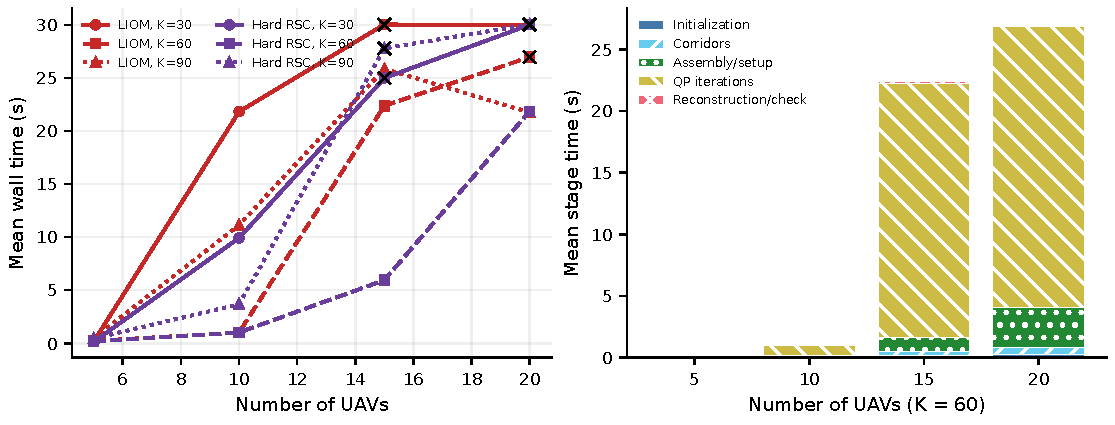
\includegraphics[width=\fulllength]{figures_revision/scaling_breakdown.pdf}
\caption{Team/grid scaling and planning-time components. Crosses mark team--grid groups with at least one attempt not accepted within 30 s. The stage breakdown includes initialization, corridor construction, assembly and solver setup, QP iterations, and final checking.\label{fig:scaling}}
\end{mdframed}
\end{adjustwidth}\end{figure}


\DIFadd{The reduced-horizon study }\DIFaddend varies $T_f$ from 8 to 12 s \DIFdelbegin \DIFdel{; the other fixes $T_f=12$ s and varies the spatial-box face-growth cap $\ell_s$ from 0.15 to 1.50 m. Both retain $K=60$ and the common physical limits. Each sweep contains 30 settings across six base layouts, with six shared default settings. The growth cap controls local corridor freedom; physical obstacle geometry is unchanged.
Proposed LIOM }\DIFdelend \DIFaddbegin \DIFadd{on six fixed geometries with unchanged corridor-growth caps. The accompanying records contain the candidate checks, outer rounds, and stopping outcomes for every method and setting.
}




\subsection{\textcolor{RevisionBlue}{Mechanism and Parameter Studies}}


\DIFadd{A separate entry-budget study varies the initial hard-QP allowance between 1}\DIFaddend , \DIFdelbegin \DIFdel{Hard-once}\DIFdelend \DIFaddbegin \DIFadd{3}\DIFaddend , and \DIFdelbegin \DIFdel{Hard RSC-QP use the same cap in each setting,and all failed attempts remain in the counts. }\DIFdelend \DIFaddbegin \DIFadd{5 s on the ten tasks used in Table~\ref{tab:external}. All other settings and the total planning budget remain fixed. Table~\ref{tab:entry-budget} reports the complete runs, including recovery after the entry solve. In C29, the 3 s entry returns directly and reduces total time from 19.27 to 3.63 s and QP calls from five to one. The 3 s setting also returns accepted 15- and 20-UAV motions within budget in this study. Giving the initial hard problem 5 s reduces the time available for subsequent recovery: Winding A then returns its accepted motion after the total budget. The 3 s allowance offers a useful compromise and is recommended for new runs. The earlier benchmark and scaling records retain their original 1 s allowance; their recorded times are unchanged.
}\DIFaddend 


\DIFdelbegin 
\begin{table}[htbp]
\begin{adjustwidth}{-\extralength}{0cm}
\begin{mdframed}[linecolor=RevisionRed,linewidth=.65pt,innerleftmargin=2pt,innerrightmargin=2pt,innertopmargin=3pt,innerbottommargin=3pt]
\color{RevisionRed}
\setlength{\textwidth}{\linewidth}\setlength{\fulllength}{\linewidth}

\caption*{\textcolor{RevisionRed}{Deleted:} Acceptance under time and spatial-corridor pressure. Each sweep contains 30 parameter settings across six base layouts.}
\small\begin{tabularx}{\fulllength}{Yrrr}
\toprule Sweep & \textbf{Proposed LIOM} & Hard-once & Hard RSC-QP \\
\midrule
Flight horizon, 8--12 s & 27/30 & 20/30 & 26/30 \\
Spatial-box growth cap, 0.15--1.50 m & 30/30 & 20/30 & 25/30 \\
\bottomrule\end{tabularx}
\end{mdframed}
\end{adjustwidth}
\end{table}

%DIFDELCMD < %%%
\DIFdelend \DIFaddbegin \begin{table}[htbp]
\begin{adjustwidth}{-\extralength}{0cm}
\begin{mdframed}[linecolor=RevisionBlue,linewidth=.65pt,innerleftmargin=2pt,innerrightmargin=2pt,innertopmargin=3pt,innerbottommargin=3pt]
\color{RevisionBlue}
\setlength{\textwidth}{\linewidth}\setlength{\fulllength}{\linewidth}

\caption{Hard-entry budget ablation. Each cell gives total planning time in seconds and QP calls. All three settings share the recorded reference and a 30 s total budget, with rotated execution order. $\times$ marks no accepted motion and $\dagger$ marks late acceptance.\label{tab:entry-budget}}
\small\begin{tabularx}{\fulllength}{Yrrr}\toprule
Task & 1 s entry: time / QPs & \textbf{3 s entry: time / QPs} & 5 s entry: time / QPs\\\midrule
C01 & 1.75 / 1 & 0.95 / 1 & 0.88 / 1\\
C03 & 1.35 / 1 & 1.44 / 1 & 1.46 / 1\\
C05 & 2.84 / 1 & 2.91 / 1 & 2.89 / 1\\
C25 & 1.20 / 1 & 1.18 / 1 & 1.17 / 1\\
C27 & 24.08 / 6 & 26.15 / 6 & 28.29 / 6\\
C29 & 19.27 / 5 & 3.63 / 1 & 3.65 / 1\\
Winding A & 28.70 / 5 & 30.00 / 5 & 31.33$^{\dagger}$ / 5\\
Winding B & 30.48$^{\dagger}$ / 6 & $\times$\,30.07 / 5 & $\times$\,30.04 / 5\\
15-UAV & $\times$\,30.08 / 7 & 29.09 / 6 & $\times$\,30.66 / 6\\
20-UAV & 28.37 / 6 & 27.04 / 6 & 30.35$^{\dagger}$ / 6\\
\bottomrule\end{tabularx}
\end{mdframed}
\end{adjustwidth}\end{table}
\DIFaddend 







\DIFdelbegin \DIFdel{Table~\mbox{7} summarizes acceptance, and Figure~\mbox{9} locates the recovered settings. In the time sweep, Proposed LIOM accepts 27}\DIFdelend \DIFaddbegin \begin{table}[htbp]
\begin{mdframed}[linecolor=RevisionBlue,linewidth=.65pt,innerleftmargin=2pt,innerrightmargin=2pt,innertopmargin=3pt,innerbottommargin=3pt]
\color{RevisionBlue}
\setlength{\textwidth}{\linewidth}\setlength{\fulllength}{\linewidth}

\caption{Soft-loop acceptance feedback and motion-envelope studies on six scenes. Feedback combines tolerance tightening with an exact-kinematics finish; its components are evaluated jointly.\label{tab:mechanism-new}}
\centering\small
\begin{tabular}{lrr}\toprule
Variant & Wall (s) & QP calls\\\midrule
Aggregate, no feedback & 1.12 & 1.33\\
Aggregate + feedback & 1.12 & 1.33\\
Normalized, no feedback & 1.07 & 1.17\\
Normalized + feedback & 1.07 & 1.17\\
cube motion envelope & 1.03 & 1.33\\
hull14 motion envelope & 1.08 & 1.17\\
hull26 motion envelope & 1.16 & 1.17\\
\bottomrule\end{tabular}
\end{mdframed}
\end{table}

\DIFadd{The hard-iterative comparison holds reconstruction opportunities fixed. The hard-entry ablation compares proposed LIOM with Soft LIOM. The acceptance-feedback study examines how rejected reconstructed motions affect subsequent computation; it also records rejection reasons and additional exact-QP calls.
}



%DIF >  BEGIN FEEDBACK COUNTS
\DIFadd{The six anchor tasks are accepted under all four recovery-criterion}\DIFaddend /\DIFdelbegin \DIFdel{30, Hard-once 20/30, and Hard RSC-QP 26/30. Proposed LIOM recovers seven Hard-once failures across four layouts; independent feasibility checks confirm initial hard-box incompatibility in all seven. Nine accepted settings require multiple solves, with at most five. Compared with Hard RSC-QP, the proposed method additionally accepts the six-UAV B and seven-UAV A layouts at 8 s, while Hard RSC-QP alone accepts seven-UAV B at 10 s}\DIFdelend \DIFaddbegin \DIFadd{feedback variants. Across the eight frozen suites, 23 reconstructed soft candidates fail a physical check, in 19 attempts; 15 of those attempts later return an accepted motion within budget. The exact-finishing branch returns 9 accepted motions. Across the 1,212 attempts in the eight frozen suites, four initialization failures concern one physical scene evaluated by four methods. The static-guide fallback follows 93 SFM simulation timeouts; no scalar-timing failure is recorded in these suites. Counts refer to attempted executions, including timing repetitions.
%DIF >  END FEEDBACK COUNTS
}




\begin{table}[htbp]
\begin{adjustwidth}{-\extralength}{0cm}
\begin{mdframed}[linecolor=RevisionBlue,linewidth=.65pt,innerleftmargin=2pt,innerrightmargin=2pt,innertopmargin=3pt,innerbottommargin=3pt]
\color{RevisionBlue}
\setlength{\textwidth}{\linewidth}\setlength{\fulllength}{\linewidth}

\caption{Reference geometry and later guide availability crossed on six anchor scenes. Mean times and rounds include all attempts; task-level outcomes accompany the data.\label{tab:initialization-new}}
\centering\small
\begin{tabular}{lrrr}\toprule
Reference & Relocation guide & Wall (s) & Rounds\\\midrule
SFM + guide fallback & False & 1.09 & 1.17\\
SFM + guide fallback & True & 1.08 & 1.17\\
Straight & False & 18.76 & 9.00\\
Straight & True & 17.98 & 7.17\\
Static guide & False & 17.95 & 7.17\\
Static guide & True & 17.93 & 7.17\\
\bottomrule\end{tabular}
\end{mdframed}
\end{adjustwidth}
\end{table}





\begin{table}[htbp]
\begin{adjustwidth}{-\extralength}{0cm}
\begin{mdframed}[linecolor=RevisionBlue,linewidth=.65pt,innerleftmargin=2pt,innerrightmargin=2pt,innertopmargin=3pt,innerbottommargin=3pt]
\color{RevisionBlue}
\setlength{\textwidth}{\linewidth}\setlength{\fulllength}{\linewidth}

\caption{One-factor sensitivity on six anchor scenes, all accepted at the tested settings. Columns give mean wall time after halving or doubling one parameter; the last row uses the stated growth factors. Nominal time is 1.07 s.\label{tab:sensitivity-new}}
\centering\small
\begin{tabular}{lrr}\toprule
Changed factor & Lower value: wall (s) & Higher value: wall (s)\\\midrule
Control effort $w_a$ & 1.00 & 1.08\\
Initial defect penalty & 1.08 & 1.01\\
Initial slack penalty & 1.07 & 1.08\\
Defect penalty cap & 1.08 & 1.08\\
Slack penalty cap & 1.07 & 1.08\\
Normalized defect tolerance & 1.07 & 1.07\\
Mean slack tolerance & 1.07 & 1.07\\
Spatial growth cap & 1.06 & 1.10\\
Relative growth cap & 2.51 & 1.09\\
SFM repulsion & 1.08 & 1.09\\
SFM decay length & 1.14 & 3.60\\
SFM look-ahead & 6.06 & 1.08\\
SFM response time & 1.10 & 1.08\\
SFM tangential fraction & 1.16 & 1.07\\
Candidate row tolerance & 1.08 & 1.08\\
Penalty growth (1.5 / 5) & 1.08 & 1.08\\
\bottomrule\end{tabular}
\end{mdframed}
\end{adjustwidth}
\end{table}





\begin{table}[htbp]
\begin{adjustwidth}{-\extralength}{0cm}
\begin{mdframed}[linecolor=RevisionBlue,linewidth=.65pt,innerleftmargin=2pt,innerrightmargin=2pt,innertopmargin=3pt,innerbottommargin=3pt]
\color{RevisionBlue}
\setlength{\textwidth}{\linewidth}\setlength{\fulllength}{\linewidth}

\caption{OSQP audit on identical matrices from three anchor scenes. Readiness stopping is compared with ordinary termination at two tolerances. The feasible-column criterion is maximum linear-row violation $\leq10^{-3}$; full trajectories still require physical acceptance.\label{tab:solver-new}}
\centering\small
\begin{tabular}{lrrrrr}\toprule
QP & Termination & Row test & Max. violation & Time (s) & Iterations\\\midrule
soft & Readiness & 3/3 & 5.2e-05 & 1.94 & 6,833\\
soft & Standard ($10^{-6}$) & 3/3 & 5.2e-05 & 1.96 & 6,833\\
soft & Standard ($10^{-7}$) & 3/3 & 1.4e-05 & 6.40 & 20,000\\
hard & Readiness & 2/3 & 1.5e+10 & 1.64 & 5,808\\
hard & Standard ($10^{-6}$) & 2/3 & 1.5e+10 & 4.10 & 13,767\\
hard & Standard ($10^{-7}$) & 2/3 & 1.5e+10 & 4.93 & 16,308\\
rsc & Readiness & 3/3 & 8.7e-04 & 0.45 & 1,400\\
rsc & Standard ($10^{-6}$) & 3/3 & 1.6e-15 & 1.37 & 4,733\\
rsc & Standard ($10^{-7}$) & 3/3 & 1.6e-15 & 2.80 & 9,283\\
\bottomrule\end{tabular}
\end{mdframed}
\end{adjustwidth}
\end{table}



\DIFadd{The initializer study crosses SFM, straight geometry, and static-guide geometry with guide availability during later relocation. It separates reference construction from the use of a guide after the initial solve. Penalty, tolerance, corridor-size, and SFM sensitivity tests change one factor at a time on six anchor tasks. Corridor-size changes are treated as a numerical sensitivity study; the physical-congestion comparisons retain the nominal limits. The motion-envelope study compares the original cube with 14- and 26-vertex inner approximations. The acceptance study compares aggregate and normalized recovery criteria, with and without acceptance feedback}\DIFaddend .

\DIFdelbegin 
\begin{figure}[!htb]
\begin{adjustwidth}{-\extralength}{0cm}
\begin{mdframed}[linecolor=RevisionRed,linewidth=.65pt,innerleftmargin=2pt,innerrightmargin=2pt,innertopmargin=3pt,innerbottommargin=3pt]
\color{RevisionRed}
\setlength{\textwidth}{\linewidth}\setlength{\fulllength}{\linewidth}

\centering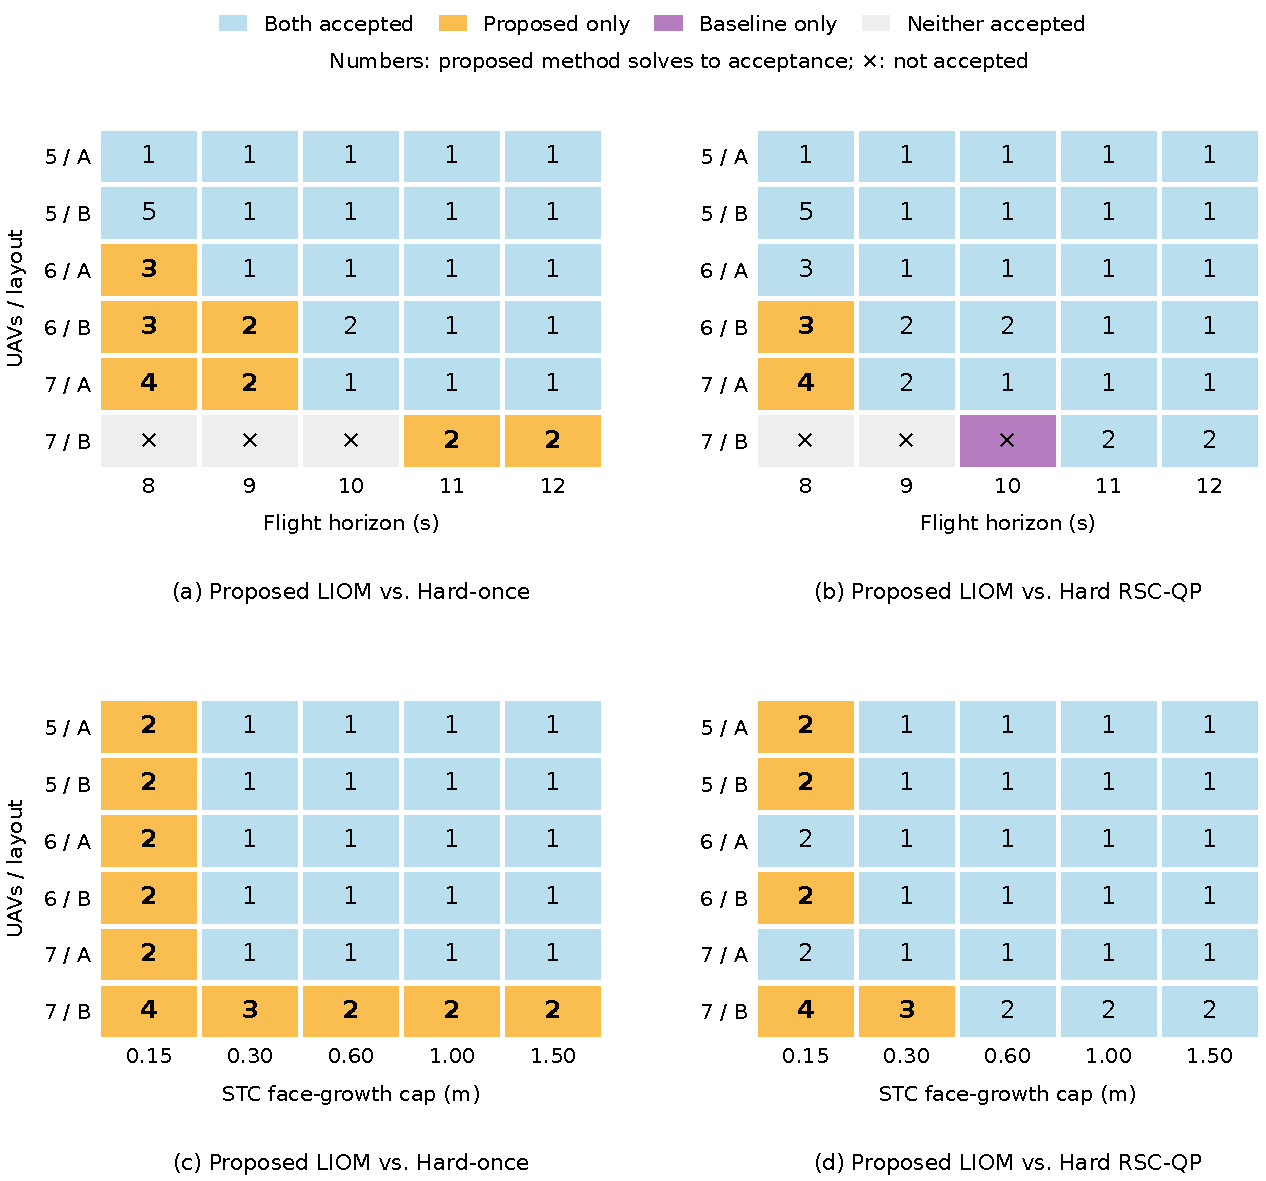
\includegraphics[width=\fulllength]{old_assets/figures_rest/pressure_sweep.pdf}
\caption*{\textcolor{RevisionRed}{Deleted:} Acceptance across the pressure grids. The upper row varies flight time; the lower row varies spatial-box freedom. A/B denote the two geometric realizations. Colors compare Proposed LIOM with each indicated baseline. Numbers give the proposed method's solves to acceptance; a cross marks its unaccepted attempt.}
\end{mdframed}
\end{adjustwidth}
\end{figure}

%DIFDELCMD < %%%
\DIFdelend \DIFaddbegin \FloatBarrier
\DIFaddend 

\DIFdelbegin \DIFdel{The spatial-box sweep more clearly separates the methods: Proposed LIOM accepts 30}\DIFdelend \DIFaddbegin \subsection{\textcolor{RevisionBlue}{Rigid-Body Tracking in a Physics Simulator}}

\label{sec:tracking}
\DIFadd{After centralized planning, each UAV receives its time-indexed position, velocity, and acceleration reference. A shared execution clock preserves their temporal coordination. Individual feedback controllers track these references; all inter-UAV decisions have already been coupled in the centralized solve. This architecture assumes known initial states and a common static map.
}


\begin{figure}[!htbp]
\begin{adjustwidth}{-\extralength}{0cm}
\begin{mdframed}[linecolor=RevisionBlue,linewidth=.65pt,innerleftmargin=2pt,innerrightmargin=2pt,innertopmargin=3pt,innerbottommargin=3pt]
\color{RevisionBlue}
\setlength{\textwidth}{\linewidth}\setlength{\fulllength}{\linewidth}
\centering
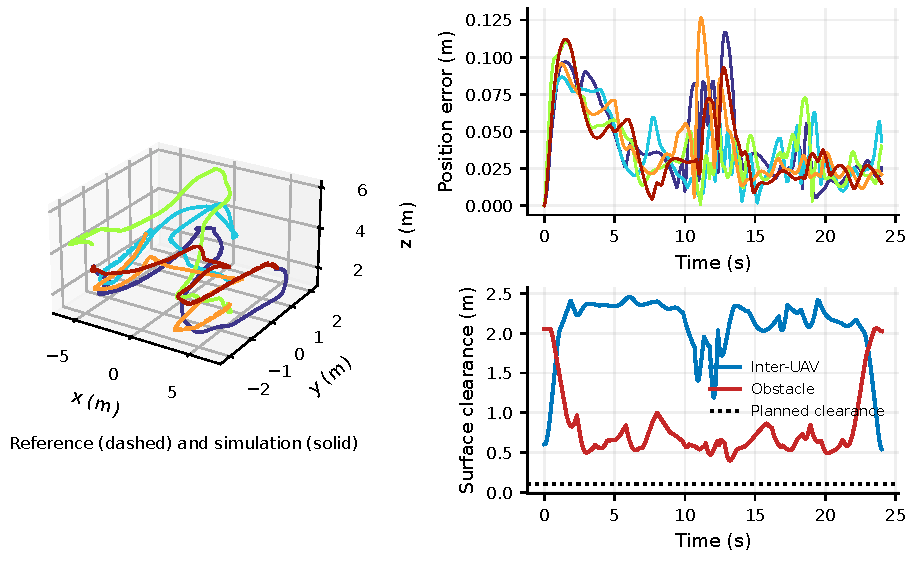
\includegraphics[width=\fulllength]{figures_revision/tracking.pdf}
\caption{Rigid-body execution of a planned cooperative motion: reference and simulated positions, tracking error, and surface clearance. Simulation measurements are sampled at the physics integration rate.\label{fig:tracking}}
\end{mdframed}
\end{adjustwidth}\end{figure}


\DIFadd{MuJoCo~\mbox{\cite{todorov2012mujoco}} provides six-degree-of-freedom rigid-body dynamics, gravity, bounded rotor actuation, motor lag, and contact detection. The generic quadrotor has mass 1 kg, inertia $\operatorname{diag}(0.006,0.006,0.010)$ kg m$^2$, rotor coordinates $(\pm0.14,\pm0.14,0)$ m, and a 5 N force limit per rotor. Motor lag is 0.02 s and the integration step is 0.002 s. Position}\DIFaddend /\DIFdelbegin \DIFdel{30 settings, Hard-once 20/30, and Hard RSC-QP 25/30. Ten settings have independently confirmed infeasible initial hard-box problems and are recovered in two to four solves.
At the smallest cap, every layout requires recovery. All five Hard RSC-QP failures are accepted by the proposed method. Once a hard local region excludes the admissible motion, the low cost of its QP alone offers no route forward. The proposed procedure instead uses intermediate candidates to relocate the corridors while preserving flight time, endpoints, and physical bounds. }\DIFdelend \DIFaddbegin \DIFadd{velocity feedback and a rotation-matrix attitude controller generate four rotor-force commands. The perturbed condition increases mass by 10\%, motor lag by 50\%, and adds sinusoidal wind force with 0.15 N amplitude per coordinate. Controller settings are fixed across the evaluated scenes.
}\DIFaddend 


The \DIFdelbegin \DIFdel{maximum observed wall times among accepted Proposed LIOM runs are 8.51 s in the time sweep and 2.03 s in the box sweep. The seven-UAV B reference exceeds the scalar timing limit at 8 s; at 9 and 10 s, numerical recovery is reached, but the reconstructed outputs do not pass the componentwise motion checks within the stopping budget}\DIFdelend \DIFaddbegin \DIFadd{simulator evaluates all accepted proposed-method motions from the first main-benchmark repetition and predetermined accepted larger-team and winding-recovery examples. The same controller is used in the nominal and perturbed conditions. Table~\ref{tab:tracking-new} reports position error, terminal accuracy at the specified completion time, separation, and contact outcomes. Full time histories, simulator models, and settings accompany the results}\DIFaddend .




\DIFdelbegin \DIFdel{Together, the sweeps demonstrate recovery across multiple layouts and degrees of local restriction. Compatible initial geometry permits a short hard-corridor solve. When that compatibility is lost, the complete recovery procedure provides intermediate candidates for geometry updates and subsequent acceptance at the unchanged flight horizon}\DIFdelend \DIFaddbegin \begin{table}[htbp]
\begin{adjustwidth}{-\extralength}{0cm}
\begin{mdframed}[linecolor=RevisionBlue,linewidth=.65pt,innerleftmargin=2pt,innerrightmargin=2pt,innertopmargin=3pt,innerbottommargin=3pt]
\color{RevisionBlue}
\setlength{\textwidth}{\linewidth}\setlength{\fulllength}{\linewidth}

\caption{MuJoCo tracking over the prescribed flight interval. Terminal error is measured at $T_f$, before the separately logged settling interval. Clearance is center distance minus two planning radii.\label{tab:tracking-new}}
\centering\small
\begin{tabular}{lrrrrrr}\toprule
Condition & Motions & Max. error (m) & Mean RMS (m) & Terminal (m) & Pair gap (m) & Contact runs\\\midrule
Nominal & 35 & 0.132 & 0.017 & 0.105 & 0.504 & 0\\
Perturbed & 35 & 0.139 & 0.057 & 0.121 & 0.469 & 0\\
\bottomrule\end{tabular}
\end{mdframed}
\end{adjustwidth}
\end{table}




\DIFadd{The closed-loop simulations assess how the planned motions are tracked under rotor-force limits, motor lag, and disturbances. Tracking errors and surface clearances characterize execution by the feedback controller. The planning model and continuous-interval checks supply the corresponding reference-motion assessment}\DIFaddend .


\DIFaddbegin \FloatBarrier


\DIFaddend \section{Conclusion}

This paper \DIFdelbegin \DIFdel{has developed a lightweight feasibility-recovery framework }\DIFdelend \DIFaddbegin \DIFadd{develops a layered solution procedure }\DIFaddend for fixed-horizon multi-UAV cooperative flight\DIFdelbegin \DIFdel{trajectory optimization in high-conflict regions. Spatial and relative corridors provide conservative linear restrictions, while separate kinematic and relative-box penalties preserve a nonempty quadratic subproblem under endpoint-compatible spatial boxes. Intermediate candidates support successive corridor reconstruction and bounded penalty updates within the prescribed flight horizon. Closed-form endpoint control correction and exact integration then produce continuous-velocity, rest-to-rest motion, with }\DIFdelend \DIFaddbegin \DIFadd{. A hard relative-corridor QP handles directly compatible local problems. Separate kinematic and relative-corridor penalties support further geometric updates when that path does not return an accepted motion. Acceptance-driven tolerance adjustment and exact finishing provide a second recovery layer. Endpoint moment correction, exact integration, and }\DIFaddend complete-interval checks \DIFdelbegin \DIFdel{determining final acceptance.
}\DIFdelend \DIFaddbegin \DIFadd{produce the returned rest-to-rest motions.
}

\DIFadd{The winding counterflow study identifies incompatible initial hard corridors and records accepted motions obtained by relaxed reconstruction at the same flight horizon. Independent phase-I checks confirm incompatibility of the initial hard constraints in two recovered layouts; the accepted continuous motions then establish feasibility of those physical tasks. The broader experiment records also contain nine accepted exact-finishing motions after soft-candidate checks fail. These observations demonstrate the role of both recovery layers. Hard relative corridors remain faster on ordinary compatible cases, motivating their direct entry into the planning procedure.
}\DIFaddend 

\DIFdelbegin \DIFdel{Controlled simulations establish second-scale planning for the tested small teams in known, static environments.
The paired comparison demonstrates lower mean computation than the tested nonlinear and sequential distance-linearization baselines, alongside the efficiency of compatible hard separating corridors . Time and corridor-pressure sweeps show the proposed method's ability to recover additional accepted motions across multiple layouts. Independent checks of initial hard-box infeasibility connect these results to the resolution of local geometric conflicts. The framework thereby combines tractable local optimization with a practical route from incompatible initial corridors to accepted cooperative flight at a fixed completion time}\DIFdelend \DIFaddbegin \DIFadd{Team and grid studies characterize computational growth through 20 UAVs. Rigid-body simulations connect the accepted plans to bounded rotor actuation and feedback tracking under disturbances. Future work will extend the known-static-map setting to rotor downwash, uncertain perception, and flight experiments}\DIFaddend .


\par
\authorcontributions{Conceptualization, Z.Y., W.T. and Z.W.; software, Y.L. and Z.Y.; investigation, Z.Y. and B.Q.; data curation, B.Q.; writing---original draft preparation, Y.L., B.Q. and Z.W.; supervision, W.T. and Z.W.; funding acquisition, W.T. and Z.W.}
\funding{This research was funded by the Fundamental Research Funds for the Central Universities, grant number 40500-20104-222624.}
\institutionalreview{Not applicable.}
\informedconsent{Not applicable.}
\DIFdelbegin %DIFDELCMD < \dataavailability{The data supporting the findings of this study are available from the corresponding author upon reasonable request.}
%DIFDELCMD < %%%
\DIFdelend \DIFaddbegin \dataavailability{The scenario definitions, planning and simulation code, raw outcomes, and analysis scripts are available at \url{https://github.com/libai1943/uav_liom}. Complete experiment archives accompany the repository release.}
\DIFaddend \conflictsofinterest{The authors declare no conflict of interest.}
\begin{adjustwidth}{-\extralength}{0cm}
\reftitle{References}
% Keep the publisher's note with the bibliography after the reference update.
\AtEndEnvironment{thebibliography}{\enlargethispage{3\baselineskip}}
\input{clean_references.bbl}
\PublishersNote{}
\end{adjustwidth}
\end{document}
